\documentclass{amsart}
\usepackage{amsmath}
\usepackage{amssymb}
\usepackage{amsthm}
\newtheorem{thm}{定理}[section]
\newtheorem{cor}[thm]{推论}
\newtheorem{prop}[thm]{命题}
\newtheorem{lem}[thm]{引理}
\newtheorem{conj}[thm]{猜想}
\newtheorem{quest}[thm]{问题}
\newtheorem{claim}[thm]{断言}

\theoremstyle{definition}
\newtheorem{defn}[thm]{定义}
\newtheorem{defns}[thm]{定义}
\newtheorem{con}[thm]{构造}
\newtheorem{exm}[thm]{例}
\newtheorem{exms}[thm]{例}
\newtheorem{notn}[thm]{记号}
\newtheorem{notns}[thm]{记号}
\newtheorem{addm}[thm]{补充}
\newtheorem{exer}[thm]{练习}

\theoremstyle{remark}
\newtheorem{rmk}[thm]{注}
\newtheorem{rmks}[thm]{注}
\newtheorem{warn}[thm]{警告}
\newtheorem{sch}[thm]{评注}


% unnumbered theorems
\theoremstyle{plain}
\newtheorem*{thm*}{定理}
\newtheorem*{prop*}{命题}
\newtheorem*{lem*}{引理}
\newtheorem*{cor*}{推论}
\newtheorem*{conj*}{猜想}

% unnumbered definitions
\theoremstyle{definition}
\newtheorem*{defn*}{定义}
\newtheorem*{exer*}{练习}
\newtheorem*{defns*}{定义}
\newtheorem*{con*}{构造}
\newtheorem*{exm*}{例}
\newtheorem*{exms*}{例}
\newtheorem*{notn*}{记号}
\newtheorem*{notns*}{记号}
\newtheorem*{addm*}{补充}


\theoremstyle{remark}
\newtheorem*{rmk*}{注}
%\usepackage{MnSymbol}
\usepackage{bm}
\usepackage{accents}
\usepackage{mathtools}
\usepackage{tikz}
\usetikzlibrary{calc}
\usetikzlibrary{decorations.pathmorphing,shapes}
\usetikzlibrary{automata,positioning}
\usepackage{tikz-cd}
\usepackage{forest}
\usepackage{braket} 
\usepackage{listings}
\usepackage{mdframed}
\usepackage{verbatim}
\usepackage{physics2}
\usephysicsmodule{ab,ab.legacy,diagmat,xmat}
\usepackage{derivative}
\usepackage{fixdif}
\usepackage{stmaryrd}
% \usepackage{euscript} 
% \usepackage[mathcal]{eucal}
\usepackage{stackengine} 
%\usepackage{/home/patrickl/homework/macaulay2}

%font
\usepackage[sc]{mathpazo}
\usepackage{inconsolata}
\usepackage{microtype}
\usepackage{xeCJK}
\setCJKmainfont{Songti SC}
\setCJKsansfont{Heiti SC}
\setCJKmonofont{Heiti SC}
\XeTeXlinebreaklocale "zh"
\XeTeXlinebreakskip = 0pt plus 1pt
% \usepackage{fontspec} 
% \setmainfont{Tex Gyre Pagella}
\usepackage[OT1,euler-digits]{eulervm}
% \usepackage{euler-math} 
\usepackage[scaled=0.86]{berasans}
% \let\sffamilyold\sffamily
% \def\sffamily{\fontencoding{T1}\sffamilyold}
% \setmonofont{Inconsolatazi4}

%CS packages
\usepackage{algorithmicx}
\usepackage{algpseudocode}
\usepackage{algorithm}

% typeset and bib
% \usepackage[english]{babel} 
% \usepackage[utf8]{inputenc} 
% \usepackage[T1]{fontenc}
\usepackage[backend=biber,style=alphabetic,maxalphanames=4,maxnames=5,hyperref,isbn=false]{biblatex}
\AtBeginBibliography{%
    \emergencystretch=3em
    \setcounter{biburlnumpenalty}{100}%
    \setcounter{biburlucpenalty}{100}%
    \setcounter{biburllcpenalty}{100}%
}
\usepackage[bookmarks, colorlinks, breaklinks]{hyperref} 
\hypersetup{linkcolor=blue,citecolor=magenta,filecolor=black,urlcolor=blue}
\usepackage{cleveref}
\usepackage{graphicx}
\graphicspath{{./}}


% other formatting packages
\usepackage{float}
\usepackage{booktabs}
\usepackage[shortlabels]{enumitem}
\setitemize{noitemsep}
\usepackage{csquotes}
%\usepackage{titlesec}
%\usepackage{titling}
%\usepackage{fancyhdr}
%\usepackage{lastpage}
% \usepackage{parskip}
\newlist{mydescription}{description}{1}
\setlist[mydescription]{style=nextline,
                        font=\bfseries,
                        % Tweak the next 4 options as needed:
                        labelindent=1cm, 
                        leftmargin =2cm,
                        rightmargin=1cm,
                        topsep     =1ex
}
\setcounter{tocdepth}{1}
\usepackage{lipsum}

% delimiters
\DeclarePairedDelimiter{\gen}{\langle}{\rangle}
\DeclarePairedDelimiter{\floor}{\lfloor}{\rfloor}
\DeclarePairedDelimiter{\ceil}{\lceil}{\rceil}



% The theorem-like environments above all share the `thm' counter, so cleveref
% names every one of them ``Theorem'' and cannot format lists of them. Alias the
% counter back to each environment and give cleveref the names.
\usepackage{etoolbox}
\crefname{thm}{定理}{定理}
\Crefname{thm}{定理}{定理}
\AtBeginEnvironment{conj}{\crefalias{thm}{conj}}
\AtBeginEnvironment{prop}{\crefalias{thm}{prop}}
\AtBeginEnvironment{lem}{\crefalias{thm}{lem}}
\AtBeginEnvironment{cor}{\crefalias{thm}{cor}}
\crefname{conj}{猜想}{猜想}
\Crefname{conj}{猜想}{猜想}
\crefname{prop}{命题}{命题}
\Crefname{prop}{命题}{命题}
\crefname{lem}{引理}{引理}
\Crefname{lem}{引理}{引理}
\crefname{cor}{推论}{推论}
\Crefname{cor}{推论}{推论}

% shortcuts
\DeclareMathOperator{\Ima}{Im}
\newcommand{\A}{\mathbb{A}}
\newcommand{\G}{\mathbb{G}}
\newcommand{\N}{\mathbb{N}}
\newcommand{\R}{\mathbb{R}}
\newcommand{\C}{\mathbb{C}}
\newcommand{\Z}{\mathbb{Z}}
\newcommand{\Q}{\mathbb{Q}}
\newcommand{\E}{\mathbb{E}}
\newcommand{\V}{\mathbb{V}}
\renewcommand{\H}{\mathbb{H}}
\renewcommand{\k}{\Bbbk}
\renewcommand{\L}{\mathbb{L}}
\renewcommand{\P}{\mathbb{P}}
\newcommand{\M}{\mathcal{M}}
\newcommand{\Mbar}{\overline{\mathcal{M}}}
\newcommand{\g}{\mathfrak{g}}
\newcommand{\h}{\mathfrak{h}}
\newcommand{\n}{\mathfrak{n}}
\renewcommand{\b}{\mathfrak{b}}
\newcommand{\ep}{\varepsilon}
\newcommand*{\dt}[1]{%
   \accentset{\mbox{\Huge\bfseries .}}{#1}}
%\renewcommand{\abstractname}{Official Description}
\newcommand{\mc}[1]{\mathcal{#1}}
% \newcommand{\msc}[1]{\mathscr{#1}}
\newcommand{\T}{\mathbb{T}}
\newcommand{\mf}[1]{\mathfrak{#1}}
\newcommand{\mbf}[1]{\mathbf{#1}}
\newcommand{\bv}{\mbf{v}}
\newcommand{\bq}{\mbf{q}}
\newcommand{\bp}{\mbf{p}}
\newcommand{\btau}{\bm{\tau}}
\newcommand{\mr}[1]{\mathrm{#1}}
\newcommand{\on}[1]{\operatorname{#1}}
\newcommand{\ms}[1]{\mathsf{#1}}
\newcommand{\mt}[1]{\mathtt{#1}}
\newcommand{\ol}[1]{\overline{#1}}
\newcommand{\ul}[1]{\underline{#1}}
\newcommand{\wt}[1]{\widetilde{#1}}
\newcommand{\wh}[1]{\widehat{#1}}
\renewcommand{\div}{\operatorname{div}}
\newcommand{\1}{\mathbf{1}}
\newcommand{\2}{\mathbf{2}}
\newcommand{\3}{\mathbf{3}}
\newcommand{\I}{\mathrm{I}}
\newcommand{\II}{\mr{I}\hspace{-1.3pt}\mr{I}}
\newcommand{\III}{\mr{I}\hspace{-1.3pt}\mr{I}\hspace{-1.3pt}\mr{I}}
\renewcommand{\v}{\mbf{v}}
\newcommand{\w}{\mbf{w}}
\newcommand{\bmu}{\bm{\mu}}
\newcommand{\pre}{\mr{pre}}
\newcommand{\vir}{\mr{vir}}
\newcommand{\fl}{\mr{fl}}
\newcommand{\ps}[1]{\llbracket #1 \rrbracket}
\newcommand{\ls}[1]{\llparenthesis #1 \rrparenthesis}
\newcommand{\loc}{\mr{loc}}

\DeclareMathOperator{\Der}{Der}
\DeclareMathOperator{\Tor}{Tor}
\DeclareMathOperator{\Hom}{Hom}
\DeclareMathOperator{\End}{End}
\DeclareMathOperator{\Ext}{Ext}
\DeclareMathOperator{\ad}{ad}
\DeclareMathOperator{\Aut}{Aut}
\DeclareMathOperator{\Rad}{Rad}
\DeclareMathOperator{\Pic}{Pic}
\DeclareMathOperator{\NS}{NS}
\DeclareMathOperator{\supp}{supp}
\DeclareMathOperator{\Supp}{Supp}
\DeclareMathOperator{\depth}{depth}
\DeclareMathOperator{\sgn}{sgn}
\DeclareMathOperator{\spec}{Spec}
\DeclareMathOperator{\Spec}{Spec}
\DeclareMathOperator{\proj}{Proj}
\DeclareMathOperator{\Proj}{Proj}
\DeclareMathOperator{\ord}{ord}
\DeclareMathOperator{\Div}{Div}
\DeclareMathOperator{\Bl}{Bl}
\DeclareMathOperator{\coker}{coker}
\DeclareMathOperator{\ev}{ev}
\DeclareMathOperator{\st}{st}
\DeclareMathOperator{\pr}{pr}
\DeclareMathOperator{\ch}{ch}
\DeclareMathOperator{\Cont}{Cont}

\addbibresource{references.bib}

\title{对数 GLSM 及相关主题}
\author{Patrick Lei}
\date{\the\year 年\the\month 月\the\day 日}
\allowdisplaybreaks

\renewcommand{\contentsname}{目录}
\renewcommand{\abstractname}{摘要}
\renewcommand{\proofname}{证明}
\renewcommand{\figurename}{图}
\renewcommand{\tablename}{表}
\renewcommand{\refname}{参考文献}
\crefname{section}{节}{节}
\Crefname{section}{节}{节}
\crefname{subsection}{小节}{小节}
\Crefname{subsection}{小节}{小节}
\crefname{figure}{图}{图}
\Crefname{figure}{图}{图}
\crefname{table}{表}{表}
\Crefname{table}{表}{表}
\crefname{equation}{式}{式}
\Crefname{equation}{式}{式}
\begin{document}
    
\begin{abstract}
    这是我为 2026 年 7 月四川大学对数 GLSM 暑期学校各场讲座所作的现场 \TeX{} 笔记。除我自己的讲座与郭帅的两场讲座外，部分插图由 Codex 或 Claude Code 后期补入。除我的讲座外，其他讲座均以中文进行；笔记中若有翻译或内容上的错误，谨此致歉。郭帅两场讲座的笔记较为实验性，是由 AI 根据幻灯片生成的转录稿。虽然我曾让 Claude 参考其余笔记以贴近我的写作风格，仍欢迎读者指出风格不一致或内容有误之处。最后，感谢周祐正、方婷婷与温耀雄指出笔记中的错误。本文由 Codex 根据英文原版笔记翻译为中文。
\end{abstract}

\maketitle

\tableofcontents

\section{\(\Theta\)-分层（温耀雄与王彬）}%
\label{sec:Theta-stratifications}

\subsection{我们的第一个模问题}%
\label{sub:Our first moduli problem}

我们的第一个模空间是\(\P^{N-1}\)。它参数化\(\C^N\)中的一维线性子空间；等价地，它是几何商\((\C^N \setminus \{0\}) / \C^{\times}\)。在这一例子中，\(\C^N\setminus\{0\}\)中的每一条\(\C^{\times}\)轨道都是闭的。这是我们遇到的第一个几何不变量理论例子。一般而言，一个取值于集合的模问题会给每个概形\(T\)指定一族定义在\(T\)上的对象的同构类；我们可以把它看作函子
\[ F \colon (\ms{Sch}_{/S})^{\mr{op}} \to \ms{Set}. \]

\begin{exm}
    设\(C\)是一个光滑的射影曲线。然后考虑赋值
    \[
    \begin{aligned}
        F_{r,d}\colon T \longmapsto
        \Bigl\{
        E \ \Bigm|\ &
        E \text{ 是 } C\times T \text{ 上的向量丛},\\
        &\operatorname{rk}(E_{\bar t})=r,\quad \deg(E_{\bar t})=d
        \text{，对每个几何点 } \bar t\to T
        \Bigr\}\big/\!\sim,
    \end{aligned}
    \]
    其中\(E_{\bar t}=E|_{C\times\{\bar t\}}\)，而\(\sim\)表示\(C\times T\)上向量丛的同构。这个函子参数化\(C\)上向量丛族的同构类，但它仍不是正确的叠值模问题。
\end{exm}

\begin{exm}
    根据 Yoneda 引理，每一个概形\(Y\)定义了一个模问题。
\end{exm}

    然而，并非所有群胚值的模问题都能被一个概形或代数空间作为叠来表示。一个概形或代数空间的惯性群是平凡的，而模问题中的对象可能具有非平凡的自同构。例如，如果考虑\(\P^1\)上的线丛的模问题，每一个线丛都有一个完整的\(\C^{\times}\)自同构群。因此，当考虑模问题时，我们需要同时记住对象和它们之间的同构，而函子的目标应该是群胚范畴。

\begin{defn}[非正式]
    一个 \textit{叠} \(\mf{X}\)在\(S\)上是一个伪函子
    \[ (\ms{Sch}_{/S})^{\mr{op}} \to \ms{Grpd} \]
    它满足关于对象和态射在 fppf 拓扑下的下降条件。
\end{defn}

\begin{exm}
    考虑叠\(\ms{Bun}_{r,d}(C)\)，它将一个概形\(T\)映射到群胚，其对象是向量丛\(E\)在\(T\times C\)上，使得每一个几何纤维\(E_{\bar t}\)的秩为\(r\)和度为\(d\)，其态射是\(T\times C\)上的向量丛的同构。
\end{exm}

    然而，叠的范围过于宽泛；我们需要限制到能够用代数几何方法处理的一类叠。

\begin{defn}
    一个 \textit{代数叠} 是一个对角态射可表（由代数空间表示）的叠，并且存在某个概形\(U\)到它的光滑满射；这样的\(U\)称为一个图册。
\end{defn}

    注意到第一个条件意味着对于任何态射\(T \to \mf{X} \times \mf{X}\)来自一个代数空间，\(T \times_{\mf{X} \times \mf{X}} \mf{X}\)是一个代数空间。这等价于所有 Isom 层是代数空间，并意味着任何来自概形到\(\mf{X}\)的态射都是可表的。

\begin{rmk}
    对于集合而言，若存在态射\(f\colon A\to C\)和\(g\colon B\to C\)，则其纤维积为
    \[ 
        A\times_C B=\ab\{(a,b)\mid f(a)=g(b)\}. 
    \] 
    对于概形或代数空间，相同的公式描述了\(T\)点的概形-理论纤维积。对于叠，一个\(T\)点的\(2\)-纤维积\(\mf{A}\times_{\mf{C}}\mf{B}\)是一个三元组\((a,b,\phi)\)，其中\(a\in\mf{A}(T)\)，\(b\in\mf{B}(T)\)，且
    \[ 
        \phi\colon f(a)\xrightarrow{\sim}g(b) 
    \]
是\(\mf{C}(T)\)中的同构。因此，等式必须被同构替代，且该同构必须作为数据的一部分记录。
\end{rmk}


\subsection{商叠}%
\label{sub:Quotient stacks}

设\(G\)为一代数群，且\(X\)为一概形，其上具有\(G\)的左作用。

\begin{defn}
\textit{商叠} \([X/G]\)将概形\(T\)映射到对象为
    \begin{equation*}
    \begin{tikzcd}
        P \ar{r}{\varphi} \ar{d} & X \\
        T,
    \end{tikzcd}
    \end{equation*}
的图，其中\(P\to T\)是fppf拓扑下的右主\(G\)-丛，且\(\varphi\)满足\(\varphi(pg)=g^{-1}\varphi(p)\)。从\((P,\varphi)\)到\((P',\varphi')\)的态射是\(P\xrightarrow{\sim}P'\)（即\(G\)-丛）的同构，且与指向\(X\)的映射兼容。
\end{defn}

\begin{exm}
设\(\mf{X}\)为\(\C\)上的有限型光滑分离 DM 叠。若\(\mf{X}\)的一般稳定子平凡，或\(\mf{X}\)的粗模空间拟射影，则\(\mf{X}\)是一个全局商~\cite{EHKV2001}。这里，DM 叠指对角态射非分歧的代数叠；全局商指形如\([U/\on{GL}_n]\)的叠，其中\(U\)是一个代数空间，且\(\on{GL}_n\)作用其上。
\end{exm}

\begin{exer}
证明群胚\([X/G](\C)\)等价于\(G(\C)\)作用于\(X(\C)\)的行动群胚。
\end{exer}

选择每个\(G(\C)\)-轨道的一个代表元\(x_i\in X(\C)\)后，上述练习表明，作为抽象群胚（而非代数叠），我们有
\[ 
    [X/G](\C) \simeq \bigsqcup_{[x_i] \in X(\C)/G(\C)} BG_{x_i}, 
\]
其中\(G_{x_i}\)是\(x_i\)的稳定子。


\subsection{细模空间、粗模空间与良好模空间}%
\label{sub:Fine vs coarse vs good moduli spaces}

\begin{defn}
    对于一个模问题，其 \textit{细模空间} 是一个概形或代数空间\(M\)，该空间能够表示对应的函子。
\end{defn}

不幸的是，找到一个细模空间非常困难，因此我们需要弱化这一条件。

\begin{defn}
对于代数叠\(\mf{X}\)，其\textit{粗模空间}是态射\(\pi\colon\mf{X}\to M\)到代数空间的映射，满足
    \begin{enumerate}
        \item 对于每个代数空间\(Y\)，与\(\pi\)的复合诱导一个双射
        \[
            \on{Hom}(M,Y)\xrightarrow{\sim}\on{Hom}(\mf{X},Y);
        \]
        \item 对于每个代数闭域\(K\)，诱导的映射
        \[
            \pi_0(\mf{X}(K))=\ab\{\mf{X}(K)\text{ 中的同构类}\}
            \longrightarrow M(K)
        \]
是双射。
    \end{enumerate}
\end{defn}


即使这些也并不总是存在。一个良好模空间是一种不同的弱化：它用上同调的仿射条件代替了几何点上的双射要求~\cite{Alper2013}。

\begin{defn}
一个从代数叠到代数空间的拟紧态射\(q\colon\mf{X}\to X\)称为一个\textit{良好模空间}，如果
    \begin{enumerate}
        \item 该前推函子\(q_*\colon\ms{QCoh}(\mf{X})\to\ms{QCoh}(X)\)是正合的；
\item 自然映射\(\mc{O}_X\to q_*\mc{O}_{\mf{X}}\)是同构。
    \end{enumerate}
\end{defn}

\begin{table}[htpb]
    \centering
    \caption{模空间的类型}
    \label{tab:moduli-types-corrected}
    \renewcommand{\arraystretch}{1.3}
    \begin{tabular}{
        p{0.18\textwidth}
        p{0.30\textwidth}
        p{0.22\textwidth}
        p{0.20\textwidth}
}
        \toprule
        \textbf{概念}
        & \textbf{定义性质}
        & \textbf{几何行为}
        & \textbf{特征}
        \\
        \midrule
        细模空间
        & 表示相应的集合值模函子
        & 其点表示该函子所记录的对象
        & 存在万有族
        \\
        粗模空间
        & 对到代数空间的映射具有万有性，且在几何同构类上为双射
        & 每个同构类对应一个几何点
        & 遗忘自同构
        \\
        良好模空间
        & 上同调仿射，且
          \(\mc{O}_X \simeq q_*\mc{O}_{\mf{X}}\)
        & 可能把不同的非闭点等同起来
        & 在 GIT 型例子中给出\(S\)-等价
        \\
        \bottomrule
    \end{tabular}
\end{table}

这些模空间的存在性并不仅仅取决于稳定子群是否为有限或无限。例如，\(B\G_m\to\on{Spec}\C\)既是一个粗模空间，也是一个良好模空间，尽管其稳定子为\(\G_m\)。

\begin{thm}[Keel-Mori {\cite{KeelMori1997}}]
设\(\mf{X}\)为\(\C\)上的有限型代数叠。若其惯性态射
    \[
        I_{\mf{X}}
        \coloneqq
        \mf{X}\times_{\mf{X}\times\mf{X}}\mf{X}
        \longrightarrow \mf{X}
    \]
是有限态射，则\(\mf{X}\)有粗模空间。\(I_{\mf{X}}\to\mf{X}\)在几何点\(x\)上的纤维是自同构群\(\on{Aut}(x)\)。
\end{thm}

\begin{thm}[Alper--Hall--Rydh {\cite{AHR2020}}]
设
    \[
        q\colon \mf{X}\longrightarrow X
    \]
为一个良好模空间，其中\(\mf{X}\)是\(\C\)上的 Noether 代数叠，且对角态射为仿射态射。
设\(x\in\mf{X}(\C)\)为一个闭点，记其
稳定子群为\(G_x\)。

则存在一个仿射概形\(\on{Spec}A\)，配备
有\(G_x\)的作用，以及一个笛卡尔图
    \[
        \begin{tikzcd}
            {[\on{Spec}A/G_x]}
                \arrow[r]
                \arrow[d]
            & \mf{X}
                \arrow[d, "q"]
            \\
            \on{Spec}(A^{G_x})
                \arrow[r, "\mathrm{\acute{e}tale}"]
            & X,
        \end{tikzcd}
    \]
其中
    \[
        \on{Spec}(A^{G_x})\longrightarrow X
    \]
是\(q(x)\)的一个 \'etale 邻域。
\end{thm}

当\(r\geq 2\)时，模叠\(\ms{Bun}_{r,d}(C)\)局部有限型，但既非准紧致也非分离。要证明其非准紧致，选取度数为\(n\)和\(d-n\)的线丛\(L_n\)与\(M_{d-n}\)，考虑
\[
    E_n=L_n\oplus M_{d-n}\oplus\mc{O}_C^{\oplus r-2}.
\]
丛\(E_n\)包含一个度为\(n\)的线丛子丛。在固定秩和度的向量丛的任意拟紧族中，线丛子丛的度均有上界；因此当\(n\to\infty\)时，这些\(E_n\)不可能全都落在同一个拟紧子叠中。为说明该叠不分离，注意每个向量丛\(E\)都具有标量自同构\(\G_m\subset\on{Aut}(E)\)。分离代数叠的稳定子群是固有的，而\(\G_m\)并不固有。取半稳定丛的开子叠并不会使叠变得分离；它只是截取出一个有限型的有界开子叠。该开子叠有良好模空间，其闭点对应于\(S\)-等价类。

\begin{defn}[斜率稳定性]
    对于非零的向量丛\(E\)，定义其斜率为
    \[ \mu(E)=\frac{\deg E}{\on{rk}E}. \]
向量丛\(E\)是 \textit{半稳定}，当且仅当
    \[ \mu(F)\leq\mu(E) \]
    对每个非零真饱和子层\(F\subset E\)均有上述不等式；若不等式为严格不等式，则称其为\textit{稳定}。由于\(C\)是光滑曲线，向量丛的饱和子层必为子丛，因此只需对非零真子丛检验这一条件。
\end{defn}

有了上述定义，我们可以考虑开子叠\(\ms{Bun}_{r,d}^{\mr{ss}}(C)\)。秩和度固定的半稳定向量丛构成一个有界族，因此该叠是有限型的，特别地也是拟紧的。然而，由于每个对象都具有非固有的标量稳定子\(\G_m\)，它仍然不是分离的。

\begin{defn}[\(S\)-等价]
设\(E\)为一个半稳定向量丛。\(E\)的 Jordan--H\"older 过滤是
    \[ 0=J_0\subset J_1\subset\cdots\subset J_N=E \]
    使得每一个商\(J_i/J_{i-1}\)在斜率条件下均为稳定的\(\mu(E)\)。该滤子并不一定是唯一的，但其关联的分次向量丛
    \[
        \on{gr}(E)=\bigoplus_{i=1}^N J_i/J_{i-1}
    \]
    在非典范同构下是唯一的。同一半稳定向量丛的两个\(E\)和\(E'\)，当它们的斜率相同时，若满足\(\on{gr}(E)\simeq\on{gr}(E')\)，则称它们为\textit{\(S\)-等价}。
\end{defn}

现在我们考虑模空间\(M_{r,d}^{\mr{ss}}(C)\)，即在\(C\)上\(S\)等价类下的半稳定向量丛。存在一个良好模空间态射
\[
    \ms{Bun}_{r,d}^{\mr{ss}}(C)\longrightarrow M_{r,d}^{\mr{ss}}(C),
\]
且\(M_{r,d}^{\mr{ss}}(C)\)的闭点与\(S\)等价类下的半稳定向量丛一一对应。

\begin{rmk}
该定理的原始证明方法是通过构造模空间来实现的，该方法基于几何不变量理论。本系列讲座的目标是讨论一种内在方法，该方法结合了\(\Theta\)分层结构与良好模空间的存在性条件，而无需首先选择 GIT 表示。
\end{rmk}


\subsection{\(\Theta\)-分层}%
\label{sub:Theta-stratifications}

本节使用的\(\Theta\)-分层与数值不变量框架见~\cite{HLinstability}。

设\(\mf{X}\)为一个代数叠，考虑\(\Theta\coloneqq[\A^1/\G_m]\)，其中点的作用为\(\lambda\cdot z=\lambda z\)；等价地，坐标函数\(t\)的权重为\(-1\)。假设以下映射叠均为概形，则定义滤过对象的叠\(\ms{Filt}(\mf{X})\coloneqq\ms{Map}(\Theta,\mf{X})\)与分次对象的叠\(\ms{Grad}(\mf{X})\coloneqq\ms{Map}(B\G_m,\mf{X})\)。存在自然的态射
\[
    \ev_1\colon\ms{Filt}(\mf{X})\to\mf{X},
    \qquad
    \on{gr}\colon\ms{Filt}(\mf{X})\to\ms{Grad}(\mf{X}),
    \qquad
    \sigma\colon\ms{Grad}(\mf{X})\to\ms{Filt}(\mf{X}).
\]
此处\(\ev_1\)为\(1\in\A^1\)上的限制，\(\on{gr}\)由包含映射\(B\G_m=\{0\}/\G_m\hookrightarrow\Theta\)诱导，\(\sigma\)则由投影\(\Theta\to B\G_m\)诱导。特别地，\(\on{gr}\circ\sigma=\on{id}\)。我们还记\(\on{tot}=\ev_1\circ\sigma\colon\ms{Grad}(\mf{X})\to\mf{X}\)。

\begin{defn}
    一个 \textit{\(\Theta\)-分层 } 在概形代数叠\(\mf{Y}\)中是连通分量\(S\subset\ms{Filt}(\mf{Y})\)的并集，使得其限制
    \[
        \ev_1|_S\colon S\longrightarrow\mf{Y}
    \]
    为闭浸没。

    \(\mf{X}\)的一个 \textit{\(\Theta\)-分层 } 由
    \begin{enumerate}
\item 一个具有最小元\(0\)的全序集\(I\)；
\item 由\(\alpha\in I\)索引的一组递增的开子叠\(\mf{X}_{\leq\alpha}\subset\mf{X}\)，使得
        \[
            \mf{X}_{\leq\alpha}\subset\mf{X}_{\leq\beta}
            \quad\text{当 }\alpha\leq\beta,
            \qquad
            \bigcup_{\alpha\in I}\mf{X}_{\leq\alpha}=\mf{X},
        \]
        且对任意\(x\in|\mf{X}|\)，集合\(\{\alpha\in I\mid x\in|\mf{X}_{\leq\alpha}|\}\)有最小元；
\item 对于每个\(\alpha>0\)，存在一个\(S_\alpha\subset\ms{Filt}(\mf{X}_{\leq\alpha})\)的\(\Theta\)分层，满足
        \[
            \mf{X}_{<\alpha}
            \coloneqq
            \bigcup_{\beta<\alpha}\mf{X}_{\leq\beta}
            =
            \mf{X}_{\leq\alpha}\setminus\ev_1(S_\alpha).
        \]
    \end{enumerate}
    该半稳定轨迹为\(\mf{X}^{\mr{ss}}\coloneqq\mf{X}_{\leq0}\)，且该分层给出一个不交分解
    \[
        \mf{X}
        =
        \mf{X}^{\mr{ss}}
        \sqcup
        \bigsqcup_{\alpha>0}\ev_1(S_\alpha).
    \]
\end{defn}

考虑叠\(\ms{Bun}_G(C) = \ms{Map}(C, BG)\)。我们将考虑
\[ \ms{Map}(\Theta, \ms{Bun}_G(C)) = \ms{Map}(\Theta \times C, BG). \]
任何这样的映射\(f\)均等价于一个\(\G_m\)-等变主\(G\)丛\(\mc{E}\)，其定义在\(\A^1\times C\)上。当\(G=\on{GL}_n\)时，这等价于一个\(\G_m\)-等变向量丛，其定义在\(\A^1\times C\)上，等价于一个有限生成的、局部自由的\(\mc{O}_C[t]\)模
\[
    \mc{E}=\bigoplus_{w\in\Z}\mc{E}_w.
\]
根据上述约定，坐标函数\(t\)的权重为\(-1\)，因此乘以\(t\)得到映射
\[
    t\colon\mc{E}_w\longrightarrow\mc{E}_{w-1}.
\]
由于\(\mc{E}\)在\(\mc{O}_C[t]\)上局部自由，乘以\(t\)的映射是单射。

\begin{rmk}
    考虑向量丛\(E=\mc{E}|_{\{1\}\times C}\)。由于\(\G_m\)在\(\G_m\times C\)上自由作用，等变下降给出
    \[
        \mc{E}|_{\G_m\times C}\simeq P_C^*E,
    \]
    其中\(P_C\colon\G_m\times C\to C\)为投影映射。等价地，
    \[
        E\simeq\big(\mc{E}[t^{-1}]\big)_0.
    \]
    定义
    \[
        F^wE\coloneqq t^w\mc{E}_w\subset\big(\mc{E}[t^{-1}]\big)_0=E.
    \]
    由于\(t\mc{E}_{w+1}\subset\mc{E}_w\)，我们有\(F^{w+1}E\subset F^wE\)。\(\mc{E}\)的有限生成性和局部自由性意味着这是一个由子丛构成的有限、穷尽且分离的递减滤子，可表示为
    \[
        0=F^{b+1}E\subset F^bE\subset\cdots\subset F^aE=E.
    \]

    另一方面，设\(E\)为一个具有有限递减子丛滤过\(F^\bullet E\)的向量丛，使得商丛\(F^wE/F^{w+1}E\)局部自由。Rees 构造是\(\mc{O}_C[t]\)-模
    \[
        \ms{Rees}(E,F^\bullet)
        \coloneqq
        \bigoplus_{w\in\Z}t^{-w}F^wE
        \subset
        E\otimes_{\C}\C[t,t^{-1}].
    \]
    它在\(\mc{O}_C[t]\)上局部自由，且其在\(t=1\)与\(t=0\)处的纤维满足
    \[
        \ms{Rees}(E,F^\bullet)|_{t=1}\simeq E,
        \qquad
        \ms{Rees}(E,F^\bullet)|_{t=0}
        \simeq
        \bigoplus_w F^wE/F^{w+1}E.
    \]
\end{rmk}

因此，从\(\Theta\)到向量丛叠的映射等价于一个有限的\(\Z\)-权重滤过，该滤过将向量丛按子丛分解，且其关联的分次部分局部自由。


\subsection{非交换局部化}%
\label{sub:Non-abelian localization}

我们首先考虑经典情形。设\(X\)为一个带\(\G_m\)作用的光滑射影簇，设\(F\)为一个\(\G_m\)-等变完美复形，记
\[
    X^{\G_m}=\bigsqcup_\alpha Z_\alpha
\]
对于不动点轨迹的连通分量分解。在将表示环\(R(\G_m)\)局部化以使以下等变欧拉类可逆后，我们有
\[
    \chi_{\G_m}(X,F)
    =
    \sum_\alpha
    \chi_{\G_m}\ab(
        Z_\alpha,
        F|_{Z_\alpha}\otimes e(N_{Z_\alpha/X})^{-1}
    ),
\]
其中
\[
    e(N_{Z_\alpha/X})
    =
    \lambda_{-1}(N_{Z_\alpha/X}^\vee)
    =
    \sum_{i\geq0}(-1)^i[\Lambda^iN_{Z_\alpha/X}^\vee].
\]

我们现在考虑叠情形。设
\[
    \mf{X}
    =
    \mf{X}^{\mr{ss}}
    \sqcup
    \bigsqcup_\alpha\ev_1(S_\alpha)
\]
为一个\(\Theta\)-分层。由于\(\ev_1|_{S_\alpha}\)是闭浸没，我们可以将\(S_\alpha\)与其在\(\mf{X}\)中的像等同。该分层的中心为
\[
    Z_\alpha\coloneqq\sigma^{-1}(S_\alpha)\subset\ms{Grad}(\mf{X}),
\]
其中\(\sigma\colon\ms{Grad}(\mf{X})\to\ms{Filt}(\mf{X})\)由投影\(\Theta\to B\G_m\)诱导。

\begin{thm}[虚非交换局部化 {\cite[定理~5.1]{HLlocalization}}]
    设\(\mf{X}\)为一个带\(\Theta\)-分层的准光滑导出叠
    \[
        \mf{X}
        =
        \mf{X}^{\mr{ss}}
        \sqcup
        \bigsqcup_\alpha S_\alpha,
    \]
    其中我们通过\(\ev_1\)将每个分层与其像等同，且设\(Z_\alpha\)为其中心。将切丛复形余切复形沿\(\G_m\)-权重分解为
    \[
        \L_{\mf{X}}|_{Z_\alpha}
        \simeq
        \L_\alpha^-
        \oplus
        \L_\alpha^0
        \oplus
        \L_\alpha^+,
    \]
    其中\(\L_\alpha^-\)、\(\L_\alpha^0\)与\(\L_\alpha^+\)的同调分别集中在负、零、正权重中。定义
    \[
        \E_\alpha
        \coloneqq
        \on{Sym}\ab(
            \L_\alpha^-
            \oplus
            (\L_\alpha^+)^\vee
        )
        \otimes
        \det(\L_\alpha^+)^\vee
        [-\on{rk}(\L_\alpha^+)]
        \in
        \ms{QCoh}(Z_\alpha).
    \]
    这里\(\det(\L_\alpha^+)\)和\(\on{rk}(\L_\alpha^+)\)分别表示完美复形\(\L_\alpha^+\)的行列式及其秩。我们称一个向量空间的复形为有限维的，当且仅当其所有上同调群的直和为有限维时。
    设\(F\in\ms{Perf}(\mf{X})\)。假设
    \[
        R\Gamma\ab(
            Z_\alpha,
            F|_{Z_\alpha}\otimes\E_\alpha
        )
    \]
    对任意\(\alpha\)有限维，且对几乎所有\(\alpha\)为零。则\(R\Gamma(\mf{X},F)\)有限维当且仅当\(R\Gamma(\mf{X}^{\mr{ss}},F)\)有限维，且
    \[
        \chi(\mf{X},F)
        =
        \chi(\mf{X}^{\mr{ss}},F)
        +
        \sum_\alpha
        \chi\ab(
            Z_\alpha,
            F|_{Z_\alpha}\otimes\E_\alpha
        ).
    \]
    这里准光滑表示\(\L_{\mf{X}}\)是 Tor-幅度包含在\([-1,1]\)中的完美复形。
\end{thm}


\subsection{几何不变量理论}%
\label{sub:Geometric invariant theory}

几何不变量理论可参见~\cite{MFK1994}。下面的向量丛例子用到了 Harder--Narasimhan 滤过~\cite{HN1975}。

设\(G\)为一个约化群，\(X\)为一个带\(G\)-等变线丛\(\mc{L}\)的射影概形。该半稳定轨迹可通过希尔伯特-穆法德准则定义，其中它包含所有满足对任意共字符
\(\lambda \colon \G_m \to G\)，可定义点 
\[ x_0 = \lim_{t \to 0} \lambda(t) x \]
并定义量
\[ \mu^L(x, \lambda) \coloneqq \frac{-\on{wt}_{x_0}(\mc{L})}{\norm{\lambda}}. \]
一个点是半稳定的，当且仅当对\(G\)的所有共字符，有\(\mu^L(x, \lambda) \leq 0\)。稳定区域由满足不等式严格成立且稳定子有限的点组成。

\begin{thm}[{\cite{MFK1994}}]
    稳定和半稳定轨迹在\(X\)中是开集。此外，\(X^{\on{ss}}/G\)是一个良商，而\(X^s/G\)是一个几何商。
\end{thm}

\begin{exm}
    考虑亏格至少为\(2\)的曲线上秩\(r\)、度\(d\)的向量丛所成的模叠\(\ms{Bun}_{r,d}\)。回顾半稳定轨迹由斜率半稳定的向量丛组成。事实上，这一轨迹可以由 GIT 得到。

固定一个 ample 的线丛\(\mc{O}(1)\)在\(C\)上。则存在某个\(n_0\)，使得对所有\(n \geq n_0\)和\(E \in \ms{Bun}_{r,d}\)，\(E(n)\)全局生成。因此，我们可以考虑
    \[ H^0(C, E(n)) \twoheadrightarrow E(n). \]
若设\(V = \C^N\)，其中\(N = h^0(E(n))\)，则存在一个满射
    \[ V \otimes \mc{O}_C(-n) \twoheadrightarrow E. \]
因此，我们可以将\(E\)视为 Quot 概形的一个点。在 Quot 概形上，我们可以考虑其万有族
    \begin{equation*}
    \begin{tikzcd}
        V \otimes \mc{O}_C(-n) \ar[twoheadrightarrow]{r} \ar{d} & \mc{E} \\
        \ms{Quot}_{V \otimes \mc{O}_C(-n), p_E} \times C \ar{r}{p} & \ms{Quot}_{V \otimes \mc{O}_C(-n)}.
    \end{tikzcd}
    \end{equation*}
现在定义线丛
    \[ \mc{L} \coloneqq \det R^0 p_* (\mc{E}(m)) \]
对于某个\(m \gg 0\)，我们也可以考虑在 Quot 概形上的\(\mr{SL}(V)\)作用。对于某个 cocharacter \(\lambda\)，我们可以将其分解
    \[ V = V_1 \oplus V_2 \]
带有权重\(s\)和\(N-s\)。
然后考虑
    \[ V_1 \otimes \mc{O}_C(-n) \subset V \otimes \mc{O}_C(-n) \twoheadrightarrow E \]
并考虑其分层
    \[ 0 \to F^1 E \to E \to E / F^1 E \to 0 \]
由该分层诱导的结构。然后我们看到
    \[ \lim_{t \to 0} \lambda(t) E = F^1 E \oplus E/F^1 E. \]
接着计算限制\(\mc{L}_{|\on{gr}_F E}\)并得到空间\(H^0(C, F^1 E(m))\)和\(H^0(C, E(m)/F^1 E(m))\)，因此\(\mc{L}\)的权重由
    \[ (N-s) p_{F^1 E}(m) - s p_{E/F^1 E}(m), \]
这恢复了 GIT。
\end{exm}

我们现在考虑不稳定轨迹。设\(E\)为\(C\)上的向量丛。则存在唯一的分层
\[ 0 \subset F^{\ell} E \subseteq \cdots \subseteq F^0 E = E \]
使得
\begin{enumerate}
    \item 所有\(\on{gr}_F^i E\)都是半稳定；
\item 对于所有\(i\)，有\(\mu(\on{gr}_F^i E) > \mu(\on{gr}_F^{i-1} E)\)。
\end{enumerate}
\begin{rmk}
从 GIT 视角来看，我们应将\(\mu\)视为约化 Hilbert 多项式。
\end{rmk}

\subsection{构造\(\Theta\)-分层}%
\label{sub:Construction of Theta-stratifications}

设\(\mf{X}\)为一合理的代数叠。\footnote{ 这里“合理”指类似于局部有限表示且对角满射为拟紧的含义。} 现在考虑\(\mc{E}\)在\(\A^1 \times C\)上的族。若限制在中心纤维上，我们发现\(\G_m\)作用于\(\on{gr}_F E\)，这意味着存在态射\(\G_m \to \Aut \on{gr}_F E\)，并由此可计算其权重。

注意，态射\(\sigma \colon \ms{Grad}(\mf{X}) \to \ms{Filt}(\mf{X})\)是一个\(\Theta\)-收缩，因此
\[ \pi_0(\ms{Filt}(\mf{X})) = \pi_0(\ms{Grad}(\mf{X})). \]

\begin{exm}
设\(\mf{X} = BG\)。则有
    \[\ms{Filt}(\mf{X}) = \bigsqcup_{[\lambda]} B P_{\lambda}, \]
其中\(P_{\lambda}\)是与 cocharacter \(\lambda\)对应的抛物子群，且我们总能在单个 Weyl 室中选择代表元。此外，我们有
    \[ \ms{Grad}(\mf{X}) = \bigsqcup_{\lambda \in \mathbb{X}_*(T)/W} B L_{\lambda}, \]
其中\(L_{\lambda}\)是与\(\lambda\)对应的 Levi 子群。
\end{exm}

\begin{defn}
\textit{\(\Theta\)-层} 在\(\mf{X}\)中是一组连通分量的并\(S \subseteq \ms{Filt}(\mf{X})\)，使得
    \[ \ev_1 \colon S \to \mf{X} \]
是闭浸入。
\end{defn}

粗略地说，闭浸没是单射，因此一个对象在\(S\)中由一个对象在\(\mf{X}\)和一个「标准纤维层」组成。

\begin{defn}
\textit{\(\Theta\)-分层} 是一族递增的开子叠
    \[ \mf{X}_{\leq c} \subseteq \mf{X}, \qquad c \in \Gamma, \]
其中\(\Gamma\)是某个全序集，且包含\(\Theta\)-层
    \[ S_c \subseteq \ms{Filt}(\mf{X}_{\leq c}), \]
这些层需满足
    \[ \mf{X}_{\leq c} = \ev_1(S_c) \sqcup \bigcup_{c' < c} \mf{X}_{\leq c'}. \]
特别地，这表明
    \[ \mf{X} = \mf{X}^{\mr{ss}} \sqcup \bigsqcup_{c > 0} \ev_1(S_c). \]
\end{defn}

类似于 Hilbert-Mumford 判别准则，我们将使用数值不变量构造\(\Theta\)-分层。
\begin{defn}
\textit{一个数值不变量} \(\mu\)，其取值在全序集\(\Gamma\)中，由一个赋值给出的缩放不变函数构成
    \[ \mu \colon \R^q \setminus \ab\{0\} \to \Gamma \]
对任意\(p \in \mf{X}(\C)\)和非退化同态\(\gamma \colon \G_m^q \to \Aut(p)\)。这些需满足
    \begin{enumerate}
\item 该赋值在域扩张下保持不变。这一观点不再展开，因为我们是在\(\C\)上工作；
\item 若存在\(\G_m^q \hookrightarrow \G_m^n \hookrightarrow \Aut(p)\)，则存在一个分解\(\R^q \setminus \ab\{0\} \to \R^n \setminus \{0\} \to \Gamma\)；
\item 若存在\(\xi \colon S \to \mf{X}\)及\(\gamma \colon \G_{m, S}^q \to \Aut(\xi)\)且核为有限群，则函数\(\mu_{\kappa(s)}\)在\(S\)上局部常值，其中\(s\)遍历\(S\)的点。
    \end{enumerate}
\end{defn}

我们将给出一个基于数值不变量\(\mu\)的构造的朴素版本。定义\(x \in \mf{X}\)为半稳定，当且仅当对于任意满足\(f(1) = x\)的非退化\(f \in \ms{Filt}(\mf{X})\)，均有\(\mu(f) \leq 0\)。若\(x\)为不稳定，则我们定义其不稳定度
\[ M^{\mu}(x) \coloneqq \sup \ab\{ \mu(f) \mid f \in \ms{Filt}(\mf{X}), \ev_1(f) = x\}. \]
若一个纤维层\(f\)达到该上确界，则称其为「Harder--Narasimhan 滤过」。

\begin{defn}
数值不变量\(\mu\)为 \textit{ 标准 } 当且仅当
    \begin{enumerate}
\item 对于\(x \in \R^q \setminus \ab\{0\}\)，\(\mu(x)\)和\(\mu(-x)\)不能同时为正；
\item 每个函数\(\mu_{\gamma}\)严格拟凹，即对于所有\(\delta \in [0,1]\)及线性无关的\(x_0, x_1 \in \R^q\)满足\(\mu(x_0), \mu(x_1) \geq 0\)，则
\[\mu_{\gamma}(\delta x_0 + (1-\delta)x_1) \geq \max\ab\{\mu_{\gamma}(x_0), \mu_{\gamma}(x_1)\}.\] 若任一值严格为正，则不等式需严格成立。
    \end{enumerate}
\end{defn}

下一条件要求某种有理性。我们考虑\(\mathbb{X}_*(T)_{\R}\)，目标是寻找其有理点。这导致条件 (R)：若存在某个\(\gamma\)使得\(\mu_{\gamma}\)取正值，则其在有理点处取得最大值。

\begin{thm}[{\cite{HLinstability}}]
设\(\mf{X}\)为一个叠，\(\mu\)为满足条件 (R) 的标准数值不变量。则\(\mu\)定义了\(\Theta\)-分层当且仅当其满足以下条件：
    \begin{itemize}
        \item 对于任意离散赋值环\(R\)，其分式域为\(K\)，残余域为\(k\)，则满足\(\mu(f_K^{\mr{HN}}) \leq M^{\mu}(f_k)\)（HN-特殊化）;
        \item 对于任意有限型概形\(T\)上的态射\(B \colon T \to \mf{X}\)，存在一个准紧开子集\(\mf{X}' \subseteq \mf{X}\)，使得对于任意有限型点\(p \in T(k)\)及其\(B(p)\)的滤子\(f\)满足\(\mu(f) > 0\)，存在另一滤子\(f'\)满足\(B(p)\)且\(\mu(f') \geq \mu(f)\)，且满足\(f'(0) \in \mf{X}'\)（HN-有界性）.
    \end{itemize}
\end{thm}

此处的关键在于，标准性与条件 (R) 结合 HN-有界性蕴含存在性，而 HN-特化蕴含唯一性。



\section{对数几何简介（方婷婷与韩子健）}%
\label{sec:Intro to log geometry (方婷婷 and 韩子健)}

\subsection{动机}%
\label{sub:Motivation}

在枚举几何中，我们将考虑在紧化模空间上的交数。这将要求我们的对象以某种方式退化，例如域曲线为节点，映射进入边界曲线，或退化目标。在普通几何中，我们将这些视为奇点，但在对数几何中，可以将这些情况视为 \textit{对数光滑}。在对数几何中，我们将函数替换为函数及其在边界（即态射\(\alpha \colon M_X \to \mc{O}_X\)）上消失的数据。

\begin{exm}
考虑一个曲线族\((xy=t)\)在\(\A^1\)上，其中中心纤维为节点。在对数几何中，若我们在\(\A^1\)上放置对数结构，则该族为对数光滑。
\end{exm}

\subsection{幺半群}%
\label{sub:Monoids}

\begin{defn}
一个 \textit{幺半群} 是具有单位元的可交换半群。
\end{defn}

对于一个幺半群\(P\)，我们可以通过标准的 Grothendieck 构造关联一个群\(P^{\mr{gp}}\)。
\[ P^{\mr{gp}} = \ab\{(a,b) \mid (a,b) \sim (c,d)\text{，若存在 }s \in P\text{ 使得 }a+d+s = b+c+s \}. \]
\begin{defn}
若自然的态射\(P \hookrightarrow P^{\mr{gp}}\)为单射，则称\(P\)为 \textit{整}。
\end{defn}

\begin{exm}
若\(P\)有生成元\(a,b,c\)与关系\(a+c=b+c\)，则在\(P^{\mr{gp}}\)中有\(a = b\)，因此\(P\)不是整的。
\end{exm}

\begin{defn}
一个幺半群\(P\)是
    \begin{itemize}
\item \textit{精细} 当且仅当\(P\)有限生成且积分；
\item \textit{饱和} 当且仅当对所有\(p \in P^{\mr{gp}}\)和自然数\(n\)，若\(np \in P\)则\(p \in P\)；
\item \textit{无挠} 当且仅当\(P^{\mr{gp}}\)是无挠群；
\item \textit{尖锐} 当且仅当恒等元是唯一的可逆元。
    \end{itemize}
\end{defn}

\subsection{对数结构}%
\label{sub:Log structures}

设\(X\)为一个概形。
\begin{defn}
在\(X\)上的一个 \textit{预对数结构} 是一个幺半群层\(M_X\)，其定义在\(X\)的小 \'etale 位点上，以及一个态射\(\alpha \colon M_X \to \mc{O}_X\)。若\(\alpha^{-1}(\mc{O}_X^{\times}) \simeq \mc{O}_X^{\times}\)成立（其中同构由\(\alpha\)给出），则其为 \textit{对数结构}。
\end{defn}

我们现在考虑正合列
\[ 0 \to \alpha^{-1}(\mc{O}_X^{\times}) \to M_X \to \bar{M}_X \to 0, \]
此处的商称为 \textit{特征层} 或 \textit{幽灵层}。

\begin{exm}
设\(M_X = \mc{O}_X^{\times}\)与\(\alpha\)为恒等映射。此时，对数结构不提供额外信息。
\end{exm}

\begin{exm}
设\(X\)为一个正则簇，\(D\)为一个闭子概形。令\(U = X \setminus D\)。然后定义
    \[ M_X = \mc{O}_X \cap j_* \mc{O}_U^{\times}, \]
其中\(j \colon U \to X\)为开浸没。若\(D\)为除子，则称为 \textit{除子对数结构}。

例如，若\(X = \A^1\)且\(D = \ab\{0\}\)，则特征层除原点外处处消失。此处，我们计算
    \[ M_X = \ab\{ \varphi \cdot t^n \mid \varphi \in \mc{O}_X^{\times} \}. \]
茎在原点以外处处为\(\mc{O}_X^{\times}\)，而在原点处为\(\mc{O}_{\A^1, 0}^{\times} \oplus \N\)。
\end{exm}

\begin{exm}
现在令\(X = \A^2\)和\(D\)为坐标轴的并集。则
    \begin{align*}
        M_{X,D} &= \ab\{f \in k[x,y] \mid f \text{ 在 } D \text{ 外可逆}\} \\
        &= \ab\{\varphi \cdot x^a \cdot y^b\}.
    \end{align*}
在一般点处，我们有\(M_p = \mc{O}_{X,p}^{\times}\)；在原点处，我们有\(\mc{O}_{X,p}^{\times}\oplus \N^2\)。在\(x\)轴上的一般点处，我们有\(x^a\)可逆，因此在该点的茎为\(\mc{O}_{X,p}^{\times}\oplus \N \cdot b\)。类似地，我们可以在\(y\)轴上的一般点处计算茎。
\end{exm}

正如我们可以将一个预层关联到一个层，我们也将一个对数结构关联到一个预对数结构。首先，在一个范畴\(\mc{C}\)中，一个推导将用\(B \sqcup_A C\)表示，并且是该图的余极限。
\begin{equation*}
\begin{tikzcd}
    A \ar{r}{f} \ar{d}[swap]{g} & B \\
    C.
\end{tikzcd}
\end{equation*}
当\(\mc{C}\)是可交换的幺半群时，
\[ B \sqcup_A C = (B \oplus C)/\sim, \qquad (f(a) + b, c) \sim (b, g(a)+c). \]

\begin{exm}
    考虑态射态射\(2 \colon \N \to \N\)和\(3 \colon \N \to \N\)。此时推出（pushout）即为幺半群
    \[ P = \frac{\N \oplus \N}{(3, 0) \sim (0,2)} \simeq \N \setminus \{1\}. \]
\end{exm}

若将\(\mc{C}\)替换为层的交换幺半群类别，则可构造截面的推出并进行层化处理。

\begin{defn}
    预对数结构\(\alpha \colon M_X \to \mc{O}_X\)的\textit{伴随对数结构}定义为推出
    \[ M_X \sqcup_{\alpha^{-1}(\mc{O}_X^{\times})} \mc{O}_X^{\times}. \]
到\(\mc{O}_X\)的映射由\((a,b) \to \alpha(a) b\)给出。
\end{defn}

\begin{defn}
    log 概形\((X, M_X) \to (Y, M_Y)\)之间的态射由以下数据组成：
    \begin{enumerate}
        \item A 态射\(\ul{f} \colon \ul{X} \to \ul{Y}\)的概形；
        \item 一个映射\(f^{\flat} \colon f^* M_Y \to M_X\)，其中\(f^* M_Y\)是与\(f^{-1} M_Y\)相关联的对数结构对数结构。
    \end{enumerate}
\end{defn}

\begin{defn}
一个对数概形 \textit{ 的 } 图表概形\((X, \alpha \colon M_X \to \mc{O}_X)\)是从常值幺半群\(P_X \to M_X\)的态射态射，使得\(M_X \simeq P_X^a \simeq P_X \oplus_{\alpha_P^{-1}(\mc{O}_X^{\times})} \mc{O}_X^{\times}\)，其中\(\alpha_P \colon P_X \to M_X \to \mc{O}_X\)。
\end{defn}

图表在描述对数结构对数结构时非常有用。例如，若我们有\(P_X \to \mc{O}_X\)，则\(P_X^a\)给出了簇\(X\)上的一个对数结构对数结构。

\begin{exm}
平凡的对数结构对数结构由图表\(P = \ab\{0\}\)给出。
\end{exm}

\begin{exm}
    设\(X = \Spec k\)并给出一个对数结构由\(\alpha_{\N} \colon \N \to k\)诱导，它将\(0\)映射到\(1\)，且将\(1\)映射到\(0\)。此即所谓的 \textit{标准对数点}，也可通过将\(\A^1\)上的除子型对数结构限制到原点得到。
\end{exm}

\begin{exm}
    考虑图表\(\N \to \mc{O}_{\A^1}\)，它将\(n \mapsto t^n\)。由此可恢复\(\A^1\)上相对于原点的除子型对数结构。
\end{exm}

\begin{exm}
    考虑图表\(\N^2 \to \mc{O}_{\A^2}\)，它将\((a,b) \mapsto x^a y^b\)。由此可恢复\(\A^2\)上相对于环面边界的除子型对数结构。
\end{exm}

\begin{defn}
    对数映射\(f \colon (X, M_X) \to (Y, M_Y)\)的 \textit{图表} 是一个三元组\((P_X\to M_X, Q_Y \to M_Y, Q \to P)\)，其中\(P_X \to M_X\)和\(Q_Y \to M_Y\)是图表，且满足以下交换图式
    \begin{equation*}
    \begin{tikzcd}
        Q_X \ar{r} \ar{d} & P_X \ar{d} \\
        f^* M_Y \ar{r} & M_X
    \end{tikzcd}
    \end{equation*}
    交换。
\end{defn}

\begin{defn}
一个概形\((X, M_X)\)是 \textit{有限生成、精细、整、饱和} 的，当且仅当存在一个 \'etale 的局部图表\(P_U \to M_U\)，使得对覆盖\(U \to X\)的每个开集，\(P\)分别为有限生成、精细、整或饱和的。
\end{defn}

\subsection{对数光滑性}%
\label{sub:Log smoothness}

\begin{defn}
考虑一个交换图
    \begin{equation*}
    \begin{tikzcd}
        T_0 \ar{r}{\phi} \ar{d}{j} & X \ar{d}{f} \\
        T_1 \ar{r}{\psi} & Y,
    \end{tikzcd}
    \end{equation*}
其中\(j\)是一个严格闭浸入（此处即\(M_{T_0} = j^* M_{T_1}\)）。一个态射的\(f \colon X \to Y\)对于精细对数概形是 \textit{对数光滑（分别为对数 \'etale）}，
    \begin{enumerate}
        \item 基础态射\(\ul{f} \colon \ul{X} \to \ul{Y}\)在局部上是有限表示的；
        \item 对任意上述交换图，在\(T_1\)上\'etale局部地，存在（相应地，存在唯一的）态射\(g \colon T_1 \to X\)，使得\(\phi = g \circ j\)且\(\psi = f \circ g\)。
    \end{enumerate}
\end{defn}

我们现在将给出一个局部图表准则，用于判断对数光滑性。

\begin{thm}[{\cite[定理~3.5]{Kato1989}}]
    设\(f \colon X \to Y\)为精细 log 概形之间的态射。假设已有图表\(Q \to M_Y\)，其中\(Q\)是精细幺半群。则\(f\)为对数光滑，当且仅当在\(X\)上\'etale局部地存在一个延拓\(Q \to M_Y\)的\(f\)的图表，并满足
    \begin{enumerate}
        \item 核与\(Q^{\mr{gp}} \to P^{\mr{gp}}\)的挠部分为有限群，其阶在\(X\)上可逆；
\item 诱导的态射\(\ul{X} \to \ul{Y} \times_{\Spec \Z[Q]} \Spec \Z[P]\)在经典意义上是 \'etale 的。
    \end{enumerate}
\end{thm}

\begin{exm}
    设\(X\)为由\(\Spec \C[P]\)给出的仿射簇，其中\(P\)是一个幺半群。注意\(P^a \simeq M_{X, X \setminus T}\)诱导了除子式的对数结构。然后考虑映射\(f \colon X \to \mr{pt}\)，其中该点具有平凡的对数结构。我们指出态射\(0 \to P^{\mr{gp}}\)无核且余核为无挠的，且该映射
    \[ \ul{X} \to \Spec \C \times_{\Spec \Z} \Spec \Z[P] = \Spec \C[P] \]
    是同构，因此任何仿射簇在平凡对数结构的点上都是对数光滑的。
\end{exm}

从这个例子中，我们可以将对数光滑性想象为相对于底的局部对数簇。

\begin{exm}
    回顾\(xy = t\)族，其相对于\(\A^1\)中心纤维的对数结构，以及相对于\(0\)的除子式对数结构。我们考虑的图表映射实际上是\(\Delta \colon \N \to \N^2\)。经过群化后，该映射变为\(\Delta \colon \Z \to \Z^2\)。由于核为平凡且余核为无挠，因此我们验证了第一个条件。然后考虑映射
    \[ \ul{X} \to \Spec \C[t] \times_{\Spec \Z[\N]} \Spec \Z[\N^2] = \Spec \frac{\C[u,v,t]}{uv-t}, \]
是同构，因此该族是对数光滑。
\end{exm}

\subsection{对数结构的叠}%
\label{sub:Stack of log structures}

对数结构的叠及其与对数光滑性的关系由 Olsson~\cite{Olsson2003} 建立。

设\(S\)为一精细对数概形。我们考虑范畴\(\ms{Log}_S\)，其对象为精细对数概形\((T, M_T) \to S\)，而其态射则为\(S\)上的严格态射\((T, M_T) \to (T', M_{T'})\)。
\begin{enumerate}
    \item 范畴\(\ms{Log}_S\)是\(\ms{Sch}_{/S}\)上的群胚纤维化范畴，它分类所有映到\(S\)的精细 log 概形；
\item \(\ms{Log}_S\)是一个代数叠，局部有限型地覆盖于\(S\)；
\item 一个态射\(f \colon X \to S\)是对数光滑当且仅当\(X \to \ms{Log}_S\)是光滑。若将光滑替换为 \'etale，则结论相同。
\end{enumerate}

\subsection{热带化}%
\label{sub:Tropicalization}

设\(X\)为精细 log 概形。则\(X\)的热带化定义为余极限
\[\Sigma(X) \coloneqq \bigsqcup_{x \in X} \Hom(\bar{M}_{X,x}, \R_{\geq 0}) \biggm/ \sim, \]
其中等价关系由下给出：若一点\(x\)退化至\(y\)，则由诱导映射\(\sigma_x \to \sigma_y\)产生的映射将\(\sigma_x\)映射到其像。

现在假设\(X\)被分层为\(X_i\)，使得\(\bar{M}_{|X_i}\)为常数。对任意的\(X_i\)，所有点\(x \in X_i\)满足\(x \in \ol{\ab\{\eta_{X_i}\}}\)，因此只需考虑各层的通用点并粘合各面。

\begin{exm}
    考虑赋予平凡对数结构的\(X\)。注意，对任意点\(x \in X\)，均有\(\bar{M}_{X,x} = 0\)，因而\(\sigma_X = \ab\{0\}\)。于是\(\Sigma(X) = \ab\{0\}\)。
\end{exm}

\begin{exm}
    考虑相对于原点的\(\A^1\)（赋予除子对数结构）。容易看出\(\sigma_0 = \Hom(\N, \R_{\geq 0}) = \R_{\geq 0}\)且\(\sigma_{\eta} = \ab\{0\}\)，因此其热带化为\(\R_{\geq 0}\)。
\end{exm}

\begin{exm}
    考虑赋予环面对数结构的\(\A^2\)（即相对于\(xy = 0\)的除子对数结构）。此时\(\sigma_{(0,0)} = \R^2_{\geq 0}\)、\(\sigma_{(x,0)} = \R_{\geq 0}\)、\(\sigma_{(0,y)} = \R_{\geq 0}\)，且\(\sigma_{(x,y)} = \ab\{0\}\)。因此，我们得到\(\A^2\)作为环面簇的扇，并将其视为锥复形。
\end{exm}

\begin{exm}
    设\(X_{\Sigma}\)为关于\(X_{\Sigma} \setminus T\)的除子式对数结构的簇。那么
    \[ \Sigma(X_{\Sigma}) = \Sigma, \]
因此，一条可能的口号是：对一个簇进行热带化，可以恢复普通托里克几何的结构（不包括扇形在某实向量空间中的嵌入）。
\end{exm}

\begin{exm}
    设\(X = \Spec k[x,y,t]/(xy-t^{\ell})\)为关于\(xy = 0\)的除子式对数结构。此时存在一个由
    \[ Q = \ab<e_x, e_y, e_t \mid e_x + e_y = \ell e_t>. \]
    注意到\(M_X = Q^a = Q \oplus_{\alpha^{-1}(\mc{O}_X^{\times})} \mc{O}_X^{\times}\)与\(\bar{M}_X = Q\)。因此有
    \begin{align*}
        \sigma_q &= \Hom(Q, \R_{\geq 0}) \\
        &= \ab\{ (\rho_x, \rho_y, \rho_t) \in \R_{\geq 0}^3 \mid \rho_x + \rho_y = \ell \rho_t \} \\
        &= \ab\{ (\rho_t, \rho_x) \in \R_{\geq 0}^2 \mid 0 \leq \rho_x \leq \ell \rho_t \}
    \end{align*}
在奇点\(q\)处，我们恢复了给出\(X\)作为一个簇的锥体。在\(x = 0\)的一般点\(\eta_x\)，我们观察到\(\bar{M}_{X, \eta_x} = \N e_t\)，因此\(\sigma_{\eta_x} = \R_{\geq 0}\)。类似地，我们还观察到\(\sigma_{\eta_y} = \R_{\geq 0}\)。剩下的问题在于粘合。

    注意到\(\bar{M}_{X, q} \to \bar{M}_{X, \eta_x}\)由\(e_t \mapsto e_t\)、\(e_x \mapsto \ell e_t\)以及\(e_y \mapsto 0\)给出，因此映射\(\sigma_{\eta_x} \to \sigma_q\)将\(\rho_t\)映射至\((\rho_t, \rho_x)\)，其中\(\rho_x = \ell \rho_t\)。

    给出一族带节点中心纤维的曲线族的态射\(X \to \A^1_t\)，其热带化由将锥体投影到\(\R_{\geq 0}\)上得到。
\end{exm}


\subsection{对数曲线}%
\label{sub:Log curves}

目前，所有幺半群和对数概形都可以是精细的（甚至是精细饱和的）。这是因为有两个原因：
\begin{enumerate}
    \item 若\(P\)是一个精细的幺半群，其对偶是 fs 且尖锐的；
    \item 若\(X = (\ul{X}, M_X)\)是一个精细对数概形，对于任意几何点\(\bar{x} \to X\)，存在\(\bar{x}\)的一个 \'etale 邻域，该邻域上存在一个图表。
\end{enumerate}

接下来，我们将讨论幺半群之间映射的各种几何性质。
\begin{defn}
    一个映射\(\theta \colon P \to Q\)是 \textit{整} 的，当且仅当映射\(\Spec\C[Q] \to \Spec \C[P]\)是平坦的。
\end{defn}

例如，任何非零映射\(\N \to \N\)和对角线映射\(\Delta \colon\N \to \N^2\)都是整的。若一个映射是整的，则对任意\(P \to P'\)，其幺半群\(P' \oplus_P Q\)是精细的。

\begin{exm}
推后可能不精细，例如考虑
    \[ \ab< a ,b,c \mid a+c=b+c> = \N^3 \oplus_{\N^2} \N. \]
\end{exm}

\begin{defn}
    一个\(f \colon X \to Y\)映射在精细对数概形上是几何点整的，如果在\(X\)的每一个几何点处，该映射
    \[ (f^*\bar{M}_Y)_{\bar{x}} \to \bar{M}_{X,\bar{x}} \]
是整的。
\end{defn}

\begin{defn}
    一个幺半群之间的\(P \to Q\)映射是 \textit{饱和}（饱和）的，如果对于所有的\(P \to P'\)，幺半群\(P' \oplus_P Q\)也是精细的（fs）。
\end{defn}

\begin{exm}
例如，映射\(\Delta \colon \N \to \N^2\)是饱和的，但映射\(\ell \colon \N \to \N\)不是。
\end{exm}

\begin{defn}
    fs log 概形\(S\)上的一条\textit{对数曲线}，是 fs log 概形之间的对数光滑且整的态射\(\pi \colon \mc{C} \to S\)，并要求其底层几何纤维均为约化连通曲线。
\end{defn}

\begin{prop}[{\cite{Kato1989}}]
    设\(f \colon X \to Y\)为 fs log 概形之间对数光滑且整的态射。则\(\ul{f}\)是平坦的。
\end{prop}

\begin{thm}[{\cite{FKato2000}}]
一个对数曲线的底层族是节点曲线族。
\end{thm}

\begin{exm}
设\(P = \N \setminus \ab\{1\}\)。则\(\Spec (P \to k[P])\)是对数光滑在\(k\)上，但\(\Spec k[P]\)是一个尖点。
\end{exm}

\begin{defn}
    fs 基\(S\)上的一条\textit{\(n\)-标记对数曲线}由数据\((\pi \colon \mc{C} \to S), \vec{p} = \ab\{p_i\}_{i=1}^n\)组成，并满足
    \begin{enumerate}
\item 底层族是一个预稳定曲线；
        \item \(\pi\)是 fs log 概形之间的对数光滑态射；
\item 在光滑轨迹\(U\)上的\(\ul{\pi}\)，我们有
            \[ \bar{M}_{\mc{C}}|_U \simeq \pi^* \bar{M}_S \oplus \bigoplus_{i=1}^n p_i \ul{\N}. \]
    \end{enumerate}
\end{defn}

\subsection{预稳定曲线上的典范对数结构}%
\label{sub:Canonical log structures on prestable curves}

设\(\mf{M}_{g,n}\)为\(n\)标记的预稳定曲线的模空间。那么奇异轨迹是一个正则交叉除子，因此存在一个规范的对数结构
\[ M_{\mf{M}_{g,n}}^{\on{can}} = M_{\partial \mf{M}_{g,n}}. \]
若考虑通用族\(\mf{C}_{g,n}\)，我们可以形成\(\pi^{-1}(\partial \mf{M}_{g,n}) \subseteq \mf{C}_{g,n}\)。因此，我们有一个映射
\[ \pi^* M_{\partial \mf{M}_{g,n}} \to M_{\pi^{-1}(\partial \mf{M}_{g,n})}. \]
我们也可以考虑分划\(p_i(\mf{M}_{g,n}) \subset \mf{C}_{g,n}\)，它们也定义了对数结构
\[ P_i \coloneqq M_{p_i(\mf{M}_{g,n})}. \]
因此，我们可以定义一个对数结构
\[ M_{\mf{C}_{g,n}}^{\on{can}} \coloneqq M_{\pi^{-1}(\partial\mf{M}_{g,n})} \oplus_{\mc{O}^{\times}} \bigoplus_{i=1}^n P_i. \]
然后，若考虑
\[ \pi^{\flat} \colon \ul{\pi}^{-1} M_{\mf{M}_{g,n}}^{\on{can}} \to M_{\pi^{-1}(\partial \mf{M}_{g,n})} \to M_{\mf{C}_{g,n}}^{\on{can}}, \]
我们可以将\(\pi\)抬升为对数叠的映射。

\begin{thm}[{\cite{FKato2000}}]
映射\(\pi\)是一个对数光滑整映射。
\end{thm}

\begin{defn}
    对于预稳定曲线的族\((\ul{C}/\ul{S}, \vec{p})\)，我们可以沿着以下交换图拉回
    \begin{equation*}
    \begin{tikzcd}
        \ul{C} \ar{r} \ar{d} & \mf{C}_{g,n} \ar{d} \\
        S \ar{r} & \mf{M}_{g,n}
    \end{tikzcd}
    \end{equation*}
并将左侧边赋予一个标准的对数结构
\end{defn}

\begin{rmk}
设\(\ul{S} = \Spec k\)。若\(S^{\on{can}} = \Spec (\N^r \to k)\)，则\(r\)表示\(\ul{C}\)上的节点数。在节点\(q\)处局部考虑 \'etale，对数结构的形式为
    \begin{equation*}
    \begin{tikzcd}
        \N^{r-1} \oplus \N^2 \ar{r} & k[x,y]/xy \\
        \N^{r-1} \oplus \N \ar{u}{\on{id}\oplus\Delta} \ar{r} & k \ar{u}.
    \end{tikzcd}
    \end{equation*}
\end{rmk}

\begin{thm}[{\cite{FKato2000}}]
设\((\mc{C}/S, \vec{p})\)为在 fs 基\(S\)上的\(n\)个标记点的对数曲线。则存在唯一的\(M_S^{\on{can}} \to M_S\)使得
    \begin{equation*}
    \begin{tikzcd}
        \mc{C} \ar{d} \ar{r} & \mc{C}^{\on{can}} \ar{d} \\
        S \ar{r}{a} & S^{\on{can}}
    \end{tikzcd}
    \end{equation*}
该图在 fs log 概形的范畴中是笛卡尔图。
\end{thm}

一个口号是：对数曲线是预稳定曲线与\(M_S^{\on{can}} \to M_S\)的组合。

\begin{exm}
设\(\ul{S} = \Spec k[s]\)和\(\ul{T} = \Spec k[t]\)。同时选择\(\ell \in \N\)。然后考虑该图示
    \begin{equation*}
    \begin{tikzcd}
        \Spec \frac{k{ [x,y,s] }}{xy-s^{\ell}} \ar{d} \ar{r} & \Spec \frac{k{ [x,y,s] }}{xy-s^{\ell}} \ar{d} \ar{r} & \Spec  \frac{k{[x,y,t]}}{xy-t} \ar{r}\ar{d} & \mf{C}_{g,n} \ar{d} \\
        \Spec k{[s]} \ar{r}{\ul{ \on{id} }} & \Spec {k[s]} \ar{r} & \Spec k{[t]} \ar{r} & \mf{M}_{g,n}.
    \end{tikzcd}
    \end{equation*}
    对于对数结构，考虑底左箭头对应于\(1 \mapsto \ell\)在\(\N\)上的情况。此时，左上角的幺半群变为\(\N^2 \oplus_{\N, \ell} \N\)。若记其为\(P\)，则态射\(k[P] \to k[\N]\)不是带有标准对数结构的对数曲线族，而是对数曲线族。
\end{exm}

\subsection{对数曲线的模空间}%
\label{sub:Moduli of log curves}

\begin{defn}
\(n\)个标记点的对数曲线之间的映射\((\mc{C}, S) \to (\mc{C}', S')\)是一个对\((\ell \colon \mc{C} \to \mc{C}', \Theta \colon S \to S')\)，使得\(\Theta\)严格且该图示
    \begin{equation*}
    \begin{tikzcd}
        \mc{C} \ar{d} \ar{r}{\ell} & \mc{C}' \ar{d} \\
        S \ar{r}{\Theta} & S'
    \end{tikzcd}
    \end{equation*}
是笛卡尔图。记\(\mf{M}_{g,n}^{\log}\)为参数化\(n\)个标记点的对数曲线的纤维范畴。
\end{defn}

\begin{prop}[{\cite{FKato2000,Olsson2003}}]
我们有\(\mf{M}_{g,n}^{\log} \simeq \ms{Log}_{(\mf{M}_{g,n}, M_{\mf{M}_{g,n}}^{\on{can}})}\)。
\end{prop}

特别地，对于一个概形\(\ul{T}\)，群胚\(\mf{M}_{g,n}^{\log}(\ul{T})\)参数化了对数结构\(M_T\)与对数曲线\(\mc{C} / T\)。

考虑一个对数曲线\(\pi \colon \mc{C} \to S, \vec{p}\)，其定义在\(S = \Spec (Q \to k)\)上。记\(\bar{\pi}^{\flat} \colon \bar{\pi}^* \bar{M}_S \to \bar{M}_{\mc{C}}\)。在一般点或光滑点\(\eta\)处，该态射
\[ \bar{\pi}_{\eta}^{\flat} \colon (\pi^{-1} \bar{M}_S)_{\eta} = Q \simeq \bar{M}_{\mc{C}, \eta}. \]
在标记点\(p_i \in \ol{\ab\{\eta\}}\)处，我们有\(\bar{M}_{\mc{C}, p_i} = Q \oplus \N\)。在此情况下，我们有
\[ \chi_{\eta} \colon \bar{M}_{\mc{C}, p_i} \xrightarrow{\on{pr}_1} \bar{M}_{\mc{C}, \eta} \]
拉回的特殊化映射
\[ \bar{\pi}_{p_i}^{\flat} \colon Q \hookrightarrow Q \oplus \N. \]
在节点\(q\)处，我们有\(\bar{M}_{\mc{C}, q} = Q \oplus_{\N} \N^2\)。令\(\rho_q\)表示\(1\)在\(Q\)中的像，即\(q\)处的边长或平滑参数。记\(\bar{\eta}_1\)和\(\bar{\eta}_2\)为\(q\)两条分支的一般点。则一般化映射为
\begin{align*}
    \chi_{\eta_1} \colon Q \oplus_{\N} \N^2 \to Q \qquad (q, (a,b)) \mapsto q + a \rho_q ;\\
    \chi_{\eta_2} \colon Q \oplus_{\N} \N^2 \to Q \qquad (q, (a,b)) \mapsto q + b \rho_q .
\end{align*}

\subsection{对数曲线的热带化}%
\label{sub:Tropicalization of log curves}

我们将仅考虑在 log 点\(S = \Spec(Q \to k)\)上的情形。我们将考虑锥体范畴\(\ms{Cone}\)，其对象为满足\((w, N_w)\)的对，其中\(w \subseteq N_w \otimes_{\Z} \R\)，且\(w\)是一个满维的强凸有理多面体锥。态射是映射\((w_1, N_{w_1}) \to (w_2, N_{w_2})\)，其由
\[ \chi \colon N_{w_1} \to N_{w_2} \]
满足\(\chi_{\R}(w_1) \subseteq w_2\)的条件所确定。

\begin{exm}
    设\(X\)为一 fs 对数概形，并考虑\(( (\bar{M}_{X,x}^{\vee})_{\R}, (\bar{M}_{X,x}^{\vee})_{\Z} )\)。
\end{exm}

我们现在考虑\(\ms{GCC}\)这一广义锥复形的范畴。其对象为拓扑空间\(\abs{\Sigma}\)，并附带一个作为\(\ms{Cone}\)中所有箭头均为面包含的图式的余极限的呈现。其态射为连续映射\(\abs{\Sigma} \to \abs{\Sigma'}\)，使得对于每一个\((w, N_w) \in \Sigma\)，映射\(w \to \abs{\Sigma'}\)均能通过\((w, N_w) \to (w', N_{w'})\)因式分解。

\begin{exm}
    若\(f \colon X \to Y\)为fs对数概形的态射，则映射\(\bar{f}^{\flat} \colon f^* \bar{M}_Y \to \bar{M}_X\)在热带化上诱导\(\Sigma(X) \to \Sigma(Y)\)。
\end{exm}

\begin{defn}
    一个\textit{锥复形}是广义锥复形\(\Sigma\)，并且对每个\((\sigma, N_{\sigma}) \in \Sigma\)，映射\(\sigma \to \abs{\Sigma}\)都是单射。
\end{defn}

\begin{thm}[{\cite{ACP2015}}]
若\(X\)是 fs 且在\(\ul{\C}\)上具有 Zariski 对数结构的对数光滑，则\(\Sigma(X)\)是一个锥复形。
\end{thm}

对于一个幺半群\(Q\)，我们记\(w_Q = Q_{\R}^{\vee} = \Hom(Q, \R_{\geq 0})\)及格子\(\Hom(Q, \Z) = Q_{\Z}^{\vee}\)。在一个光滑点处，我们有
\[ w_{\eta} = (Q_{\R}^{\vee}, Q_{\Z}^{\vee}). \]
在标记点处，我们看到
\[ w_p = \ab(\Hom (Q \oplus \N, \R_{\geq 0}) = Q_{\R}^{\vee} \oplus \R_{\geq 0}, Q_{\Z}^{\vee}\oplus \Z). \]
在节点处，我们有
\begin{align*}
    w_q &= \ab(\Hom(Q \oplus_{\N} \N^2, \R_{\geq 0}), ( \bar{M}_{\mc{C}, q} )_{\Z}^{\vee}).
\end{align*}
注意锥实际上等于
\[ \ab\{(m, m_x, m_y) \mid m(\rho_q) = m_x + m_y \} \simeq \ab\{(m, e_x) \mid e_x \leq m(\rho_q) \} \subseteq Q_{\R}^{\vee} \times \R_{\geq 0}. \]

现在我们理解了每个点关联的锥，接下来需要讨论面映射。与标记点对应的广义映射是
\[ Q \oplus \N \xrightarrow{\on{pr}_1} Q, \]
以及相关的面映射是
\[ w_{\eta} \hookrightarrow w_p \qquad m \mapsto (m,0). \]
在节点处，两个面映射是
\[ \chi_{\eta_1}^{\vee} \colon Q_{\R}^{\vee} \to w_q \qquad m \mapsto (m, m(\rho_q)) \]
和
\[ \chi_{\eta_2}^{\vee} \colon Q_{\R}^{\vee} \to w_q \qquad m \mapsto (m, 0). \]

\begin{exm}
    考虑一条由两条有标记点\(p\)的有理曲线组成的曲线。然后设\(\ul{S} = \Spec \C\)。此时我们发现
    \[ S^{\on{can}} = \Spec(\N \to \C), \]
    \(Q = \N\)，且\(Q_{\R}^{\vee} = \R_{\geq 0}\)。此外，我们还观察到\(\bar{M}_{C, q} = \N \oplus_{\N} \N^2\)和\(\bar{M}_{C, p} = \N \oplus \N\)。
\end{exm}

\begin{figure}[H]
    \centering
    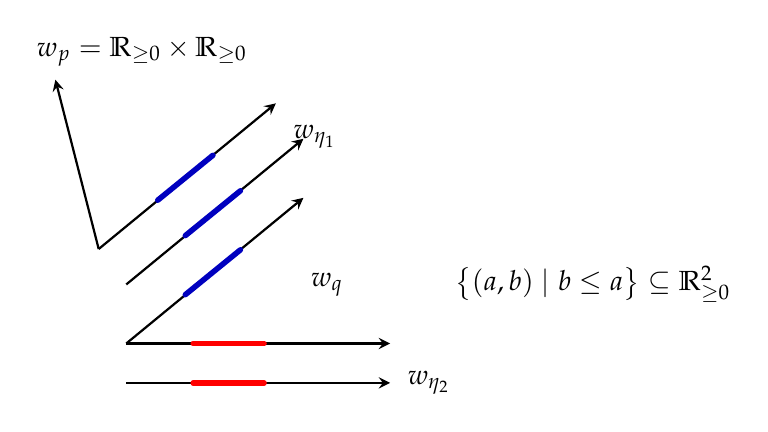
\begin{tikzpicture}[
        x=1cm,
        y=1cm,
        cone ray/.style={thick,->,>=stealth},
        common face/.style={red,line width=2pt,line cap=round},
        diagonal face/.style={blue!75!black,line width=2pt,line cap=round}
    ]
        % The cone at the marked point.
        \coordinate (p) at (0,4.45);
        \draw[cone ray] (p) -- ++(-0.55,2.15);
        \draw[cone ray] (p) -- ++(2.25,1.85);
        \draw[diagonal face]
            ($(p)+(0.75,0.62)$) -- ($(p)+(1.45,1.19)$);
        \node[above] at ($(p)+(0.55,2.2)$)
            {$w_p=\R_{\geq 0}\times\R_{\geq 0}$};

        % The cone at the first generic point.
        \coordinate (etaone) at (0.35,4);
        \draw[cone ray] (etaone) -- ++(2.25,1.85);
        \draw[diagonal face]
            ($(etaone)+(0.75,0.62)$) -- ($(etaone)+(1.45,1.19)$);
        \node[above right] at ($(etaone)+(2.0,1.6)$) {$w_{\eta_1}$};

        % The cone at the node.
        \coordinate (q) at (0.35,3.25);
        \draw[cone ray] (q) -- ++(2.25,1.85);
        \draw[cone ray] (q) -- ++(3.35,0);
        \draw[diagonal face]
            ($(q)+(0.75,0.62)$) -- ($(q)+(1.45,1.19)$);
        \draw[common face] ($(q)+(0.85,0)$) -- ($(q)+(1.75,0)$);
        \node at ($(q)+(2.55,0.75)$) {$w_q$};
        \node[anchor=west] at ($(q)+(4.05,0.75)$)
            {$\bigl\{(a,b)\mid b\leq a\bigr\}\subseteq\R_{\geq 0}^{2}$};

        % The colored intervals indicate the common faces used in the gluing.
        \coordinate (etatwo) at (0.35,2.75);
        \draw[cone ray] (etatwo) -- ++(3.35,0);
        \draw[common face] ($(etatwo)+(0.85,0)$) -- ($(etatwo)+(1.75,0)$);
        \node[right] at ($(etatwo)+(3.45,0)$) {$w_{\eta_2}$};
    \end{tikzpicture}
\end{figure}


\subsection{热带曲线}%
\label{sub:Tropical curves}

\begin{defn}
    一族 \textit{热带曲线} \((G, \vec{g}, \vec{\ell})\)在锥\(w, N_w\)上由
    \begin{enumerate}
        \item 一个连通的图\(G = V(G) \cup E(G) \cup L(G)\)构成；
        \item 一个\(\vec{m} \colon L(G) \xrightarrow{\sim} \ab\{1, \ldots, n\}\)的边序排列；
        \item 一个亏格函数\(\vec{g} \colon V(G) \to \N\)；
        \item 一个边长函数\(\ell \colon E(G) \to \Hom(w \cap N_w, \N) \setminus \ab\{0\}\)。
    \end{enumerate}
\end{defn}

现在我们构造\(\Sigma(G, \ell)\)。对于\(v \in V(G)\)，我们设定\(w_v = w\)。对于\(e \in E(G)\)，我们设定
\[ w_e = \ab\{ (s, \lambda) \mid \lambda \leq \vec{\ell}(e)(s) \} \subseteq w \times \R_{\geq 0}. \]
对于边\(\ell \in L(G)\)，我们设定\(w_{\ell} = w \times \R_{\geq 0}\)。接下来需要定义面态射。若\(\ell\)与\(v\)相关联，则面态射为
\[ w_v \hookrightarrow w_{\ell} \colon s \mapsto (s, 0). \]
若\(e\)与两个顶点\(v_1, v_2\)相关联，则面态射为
\begin{align*}
    w_{v_1} \hookrightarrow w_e &\colon s \mapsto (s, \vec{\ell}(e)(s)) \\
    w_{v_2} \hookrightarrow w_e & \colon s \mapsto (s, 0).
\end{align*}
\begin{rmk}
    选择\(v_1\)和\(v_2\)不会改变锥复形在同构下的性质，但在定义对数映射的接触阶数时则至关重要。然而，通常没有规范的方法进行此类选择。
\end{rmk}

\subsection{穿孔曲线}%
\label{sub:Punctured curves}

穿孔对数曲线与映射的理论见~\cite{ACGS2025}。

我们考虑一个有节点的曲线
\[ \Spec k[x,y]/xy \to \Spec k \]
给定模结构对数结构为\(\N^2\)，其图表为\((a,b) \mapsto x^a y^b\)且\(\N \to k\)为标准对数点。现在考虑\(\ul{C}_1 = Z(x) = \Spec k[y]\)，并标记节点\(p \colon \Spec k \to \Spec k[y]\)。注意
\[ C^{\on{can}} = (\ul{C}, M_C) \to S^{\on{can}} = \Spec(\N \to k). \]
记\(M_{C_1}^{\circ} = M_C|_{C_1}\)。则在对数结构上，我们有图示
\begin{equation*}
\begin{tikzcd}
    k[y] & & \N^2 \ar{ll}[swap]{(a,b) \mapsto 0^a y^b} \\
    k \ar{u} & & \N \ar{ll} \ar{u}{\Delta}.
\end{tikzcd}
\end{equation*}
特别地，我们可以计算茎\(\bar{M}_{C_1}^{\circ}|_p = \N^2\)，因此有
\[ \bar{\pi}_{C_1^{\circ}}^{\flat} |_p \colon \N \xrightarrow{\Delta} \N^2. \]
然而，我们应当存在映射
\[ \bar{\pi}^{\flat}_{C_1}|_p \colon \N \xrightarrow{i_1} \N \oplus \N, \]
因此，\(C_1\)不是 \textbf{ 与 } 的对数曲线。我们随后可以考虑图示
\begin{equation*}
\begin{tikzcd}
    \N \oplus \Z \\
    \N^2 \ar[hookrightarrow]{u} \ar{rr}{(0,1)\mapsto (0,1)}[swap]{(1,0)\mapsto (1,1)} & & \N^2 \ar{ull}[swap]{\Vectorstack{{(1,0)\mapsto(1,-1)} {(0,1)\mapsto(0,1)}}} \\
    & \N \ar{ul}{i_1} \ar{ur}{\Delta}.
\end{tikzcd}
\end{equation*}
因此，我们将考虑扩展对数结构。

回顾一下，对于一个对数曲线，我们有\(M_{\mc{C}} = M_{\mc{C}}' \oplus_{\mc{O}_{\mc{C}}^{\times}} P_{\mc{C}}\)，其中\(P_{\mc{C}}\)是由标记定义的除子式对数结构。

\begin{defn}
    一个 \textit{穿孔曲线} 在一个 fs log 概形\(S\)上由\((\mc{C}^{\circ} \xrightarrow{p} \mc{C} \xrightarrow{\pi} S, \{p_i\}_{i=1}^n)\)组成，其中\((\mc{C} \xrightarrow{\pi} S, \vec{p})\)是一个对数曲线，且态射\(p \colon \mc{C}^{\circ} \to \mc{C}\)满足以下精细对数概形的条件：
    \begin{enumerate}
        \item 该映射的底层映射\(\ul{p}\)是同构；
        \item 在对数结构上，映射\(p^{\flat} \colon M_{\mc{C}} \hookrightarrow M_{\mc{C}^{\circ}}\)在除\(p_i\)外的区域上是同构，并诱导
            \[ M_{\mc{C}} \xrightarrow{p^{\flat}} M_{\mc{C}^{\circ}} \hookrightarrow M_{\mc{C}} \oplus P^{\mr{gp}}. \]
        \item 对于任意标记\(p_i\)和任意\(s \in M_{\mc{C}^{\circ}, p_i} \setminus M_{\mc{C}, p_i}\)，有\(\alpha_{\mc{C}^{\circ}}(s) = 0\)。
    \end{enumerate}
\end{defn}

简言之，对数曲线穿孔曲线是对数曲线对数曲线加上一个可交换图示
\begin{equation*}
\begin{tikzcd}
    M_{\mc{C}^{\circ}} \ar{dr} \ar[hookrightarrow]{r} & M_{\mc{C}}' \oplus_{\mc{O}_{\mc{C}}^{\times}} P^{\on{gp}} \\
    & \mc{O}_{\mc{C}} \\
    M_{\mc{C}} \ar[hookrightarrow]{uu} \ar{ur}.
\end{tikzcd}
\end{equation*}


\begin{exm}
    设\((\ul{\mc{C}} \to \ul{S} = \Spec k, p)\)是一个光滑的\(1\)-标记曲线。
    \begin{enumerate}
        \item 赋予\((\mc{C}/S, p)\)典范对数结构（因此\(S\)本身没有对数结构）。令\(M_{\mc{C}} = P\)。则任意穿孔\(p^{\flat} \colon M_{\mc{C}} \hookrightarrow M_{\mc{C}^{\circ}} \subset P^{\on{gp}}\)必为平凡。原因是\(M_{\mc{C}^{\circ}}\)不可能存在截面\(s\)使得\(\alpha_{\mc{C}^{\circ}}(s) = 0\)。若\(s \in P = M_{\mc{C}}\)，则\(\alpha_{\mc{C}^{\circ}}(s) = \alpha_{\mc{C}}(s)\)；否则\(s \notin P\)，而由\(\alpha_{\mc{C}^{\circ}}(-s)\)非零可知\(\alpha_{\mc{C}^{\circ}}(s)\)也非零。
        \item 设\(M_{\mc{C}^{\circ}} \subseteq (\N \oplus \mc{O}_{\mc{C}}^{\times}) \oplus P^{\on{gp}}\)为穿孔。选择\(x\)作为\(\mc{O}(-p)\)的局部生成元。那么任意\(s \in M_{\mc{C}^{\circ}, p}\)均可表示为\(s = ((n, \varphi), x^m)\)，其中\(n \in \N\)且\(\varphi \in \mc{O}_{\mc{C}, p}^{\times}\)。若\(m < 0\)，则需满足\(\alpha_{\mc{C}^{\circ}}(s) = 0\)。这蕴含\(\alpha_{\mc{C}}((n, \varphi), 0) = 0\)，因此
            \[ \bar{M}_{\mc{C}^{\circ}, p} \subseteq \ab\{(n, m) \in \N \oplus \Z \mid n = 0 \text{ 时 } m \geq 0 \}. \]
            实际上，任何包含\(\N \oplus \N\)的右端子幺半群均可通过穿孔实现。
        \item 设\(S = \Spec(\N \to k)\)。考虑\(M_{\mc{C}^{\circ}}\)使得\(\bar{M}_{\mc{C}^{\circ}, p} = \N^2 + \N (2,-2)\)。由于\((1,-1) \notin \bar{M}_{\mc{C}^{\circ}, p}\)，可知\(M_{\mc{C}^{\circ}}\)不是饱和的。
    \end{enumerate}
\end{exm}

\begin{lem}[{\cite{ACGS2025}}]
设\(Q\)为一尖锐有限生成幺半群。设\(w \coloneqq \Hom(Q, \R_{\geq 0}) = Q_{\R}^{\vee}\)。设\(Q^{\circ} \subseteq Q \oplus \Z\)为有限生成且满足\(Q \oplus \N \subsetneq Q^{\circ}\)及\(Q^{\circ} \cap \ab\{0\} \times \Z_{<0} = \emptyset\)。此时存在一个非零、凹且分段线性的函数
    \[ \ell \colon w \to \R_{\geq 0} \]
其有有理斜率
    \[ (Q^{\circ})_{\R}^{\vee} = \ab\{ (s, \lambda) \in w \times \R_{\geq 0} \mid 0 \leq \lambda \leq \ell(s) \}. \]
\end{lem}

\begin{exm}
    设\(Q = \N^2\)，并定义
    \begin{align*}
        Q^{\circ} &= \ab<((1,0), -1), ((0,1), -1), ((0,0),1)> \subset \N^2 \oplus \Z \\
        &= \ab\{((a,b), m) \mid a+b+m \geq 0, a,b \geq 0 \}.
    \end{align*}
则
    \[ (Q^{\circ})_{\R}^{\vee} = \ab\{ (e_x, e_y, e_t) \mid 0 \leq e_t \leq \min(e_x, e_y) \}. \]
\end{exm}





\section{对高亏格的Gromov--Witten 理论入门（Patrick Lei）}%
\label{sec:Intro to GW theory with a view to higher genus (Patrick Lei)}


\subsection{Gromov--Witten 理论导论}%
\label{sub:Introduction to GW theory}

虚基本类的构造见~\cite{BehrendFantechi1997}；公理与量子上同调见~\cite{KM1994}。

这些讲座的目标，是以便于进行高亏格计算的方式介绍Gromov--Witten 理论。Gromov--Witten 理论研究模空间\(\Mbar_{g,n}(X, \beta)\)上的积分，其中\(X\)是光滑射影代数簇，而\(\beta \in H_2(X, \Z)\)是有效曲线类。我们有交换图
\begin{equation*}
\begin{tikzcd}
    \mc{C} \ar{r}{f} \ar[bend right=20]{d}[swap]{\pi} & X \\
    \Mbar_{g,n}(X, \beta) \ar[bend right=20]{u}[swap]{\sigma_i} \ar{ur}[swap]{\on{ev}_i}
\end{tikzcd}
\end{equation*}
其中\(\mc{C}\)是通用曲线，\(\sigma_i\)是\(\pi\)的截面，给出了标记点，\(f\)是通用稳定映射，而\(\ev_i = f \circ \sigma_i\)是态射的评估态射。虽然\(\Mbar_{g,n}(X, \beta)\)通常是奇异的、非等维的且可约的，但存在一个特殊类
\[ [\Mbar_{g,n}(X, \beta)]^{\vir} \in A_{\ab(c_1(X), \beta) + (\dim X - 3)(1-g) + n}(\Mbar_{g,n}(X, \beta), \Q), \]
即所谓的 \textit{虚基本类}。

\begin{exer}
    利用变形理论中的标准论证方法，验证\(\Mbar_{g,n}(X, \beta)\)的“预期维数”确实等于上文中给出的数值。
\end{exer}

当\(X\)光滑且射影时，\(\Mbar_{g,n}(X, \beta)\)是固有的，因此可以定义\textit{Gromov--Witten 不变量}
\[ \ab<\tau_{a_1}(\alpha_1), \cdots, \tau_{a_n}(\alpha_n)>_{g,n,\beta} \coloneqq \int_{[\Mbar_{g,n}(X, \beta)]^{\vir}} \prod_{i=1}^n \ev_i^* \alpha_i \cdot \psi_i^{a_i} \]
其中，\(\alpha_i \in H^*(X)\)的\(\psi_i\)由\(\psi_i = c_1(\sigma_i^*(\omega_{\pi}))\)定义

遗憾的是，计算单个 Gromov--Witten 不变量非常困难，因此我们将考虑更为困难的问题，即研究 GW 不变量的生成级数，例如
\[ F_g = \sum_{\beta \geq 0} q^{\beta} \ab<>_{g,0,\beta} \]
当\(X\)为Calabi--Yau 三维簇时。这里\(q\)是记录曲线类的形式变量，并将环\(\Q\ps{q^{\beta} \mid \beta \in H_2(X, \Z)_{\mr{eff}}}\)记作\(\Lambda\)。我们还将考虑其他一些结构。首先是\textit{量子上同调环}，其乘积\(a \star_{\mbf{t}} b\)由下式给出
\[
    (a \star_{\mbf{t}} b, c) = \sum_{\substack{\beta \geq 0 \\ n \geq 0}} \ab<a,b,c, \mbf{t}, \ldots, \mbf{t}>_{0,3+n,\beta} \frac{q^{\beta}}{n!}.
\]
这里给出\(a,b,c, \mbf{t} \in H^*(X)\)。我们还将考虑 \textit{ 量子联络 }。设\(\ab\{ e_i \}\)为\(H^*(X)\)的一组基。此时，量子联络是定义在纤维为\(H^*(X)\)的平凡丛上，其底空间为\(H^*(X) \times \P^1_z\)的联络，由以下公式给出：
\[ \nabla_{t^i} = \partial_{t^i} + \frac{1}{z} e_i \star_{\mbf{t}}. \]
有时，考虑\(z\)方向上的联络也很有用，其定义为：
\[ \nabla_{z \odv{}{z}} \coloneqq z \odv{}{z} - \frac{1}{z} E_X \star_{\mbf{t}} + \mu_X, \]
其中\(\mu_X(\alpha) = \frac{\deg(\alpha) - \dim X}{2} \alpha\)是一个分次算子，且
\[ E_X = c_1(X) + \sum_i \ab(1 - \frac{\deg(e_i)}{2})t^i e_i \]
是\textit{Euler 向量场}。由于我们主要关注Calabi--Yau 簇，因此不考虑这一点。

\subsection{亏格零的枚举镜像对称}%
\label{sub:Enumerative mirror symmetry in genus zero}

数学家们开始研究 Gromov--Witten 理论的动力源于 20 世纪 90 年代初期，当时 Candelas、de la Ossa、Green 与 Parkes~\cite{CandelasEtAl1991} 预测了在一般五次三维簇上低亏格度的有理曲线数量，其方法是将问题转化为计算另一类 Calabi--Yau 三维簇（即 \textit{mirror quintic}）上的周期积分（等价地，研究其 Hodge 结构的变体）。在亏格零情况下，所有不变量均可由 \textit{\(J\)-函数} 与\(J_{\mbf{t}}(q,z) \in H^*(X, \Lambda)[z]\)表示，该式由
\[ \ab( J_{\mbf{t}}(q, z), \alpha ) \coloneqq (z + \mbf{t}, \alpha) + \sum_{n, \beta} \frac{q^{\beta}}{n!} \ab< \frac{\alpha}{z-\psi}, \mbf{t}, \ldots, \mbf{t}>_{0,1+n, \beta} \]
对任意\(\mbf{t} \in H^*(X, \Lambda)[z]\)和\(\alpha \in H^*(X)\)，其中\((-,-)\)是 Poincar\'e 配对。因此，计算所有带后裔（即\(\psi\)类）的亏格零Gromov--Witten 不变量，归结为计算\(J\)-函数。

\begin{rmk}
我们将\(\frac{1}{z-\psi}\)展开为\(\sum_{k=0}^{\infty} \psi^k z^{-k-1}\)。
\end{rmk}

值得注意的是，\(J\)-函数可通过量子微分方程的基本解获得，其表达式为
\[ ( S_{\mbf{t}}(z) \phi , \alpha) = (\phi, \alpha) + \sum_{n, \beta} \frac{q^{\beta}}{n!} \ab<\frac{\alpha}{z-\psi}, \phi, \mbf{t}, \ldots, \mbf{t}>_{0, 2+n, \beta}. \]
该解具有性质\(S_{\mbf{t}}^*(-z) S_{\mbf{t}}(z) = \on{Id}\)，通常称为 \textit{辛性质}。由此，我们可通过\(z S_{\mbf{t}}^*(z)\cdot 1 = J_{\mbf{t}}(q, z)\)恢复\(J\)-函数。

在物理学中，镜像对称是 A 模与 B 模之间的对偶性，因此现在需要引入 B 模对象。为节省时间（及符号），我们假设\(X\)是一个 toric 簇，且\(-K_X\)为 nef。令\(D_1, \ldots, D_r\)为\(X\)中所有 torus-invariant divisors 的完整集合。然后定义\(I\)函数
\[
    I_{\mbf{t}}(q, z) \coloneqq z e^{\mbf{t}/z} \sum_{\beta \geq 0} q^{\beta} \frac{\prod_{i=1}^r \prod_{m = -\infty}^{0} (D_i + mz)}{\prod_{i=1}^r \prod_{m=-\infty}^{\beta \cdot D_i} (D_i + mz)}.
\]
此处需注意，任何出现的\((D_i + mz)^{-1}\)均可展开为\(\frac{1}{mz} \ab(1 - \frac{D_i}{mz} + \cdots)\)，即以\(\frac{D_i}{mz}\)为几何级数展开。此外，\(I\)-函数满足一个称为 \textit{Picard--Fuchs 方程} 的微分方程（属于超几何型）。

\begin{exm}
若\(\mbf{t} = 0\)与\(X = \P^1\)，我们得到
    \begin{align*}
        I(q,z) &= z\sum_{d \geq 0} q^d \frac{1}{\prod_{m=1}^d (H + mz)^2} \\
        &= z\sum_{d \geq 0} \ab(\frac{q}{z^2})^d \frac{1}{(d!^2)} + O(H),
    \end{align*}
因此，实际上，一阶贝塞尔函数是主导项。
\end{exm}

若\(X\)是簇\(Y\)中的一个线丛\(L_1, \ldots, L_k\)截取的 \textit{ 凸 } \(H^1(f^* L_i) = 0\)完全交点，且对于任意亏格零稳定映射到\(Y\)的映射均满足，则量子 Lefschetz 定理~\cite{CoatesGivental2007} 允许我们将\([\Mbar_{g,n}(X, \beta)]^{\vir}\)替换为\(e\ab(\bigoplus \pi_* f^* L_i) \cap [\Mbar_{g,n}(Y, \beta)]^{\vir}\)，并将所有计算转移到\(Y\)上进行。此时，\(I\)-函数的定义为
\[
    I_{\mbf{t}}(q,z) \coloneqq z e^{\mbf{t}/z} \sum_{\beta \geq 0} q^{\beta} \frac{\prod_{i=1}^k \prod_{m=-\infty}^{L_i \cdot \beta} (L_i + mz)}{\prod_{i=1}^k \prod_{m=-\infty}^{0} (L_i + mz)} \frac{\prod_{i=1}^r \prod_{m = -\infty}^{0} (D_i + mz)}{\prod_{i=1}^r \prod_{m=-\infty}^{\beta \cdot D_i} (D_i + mz)},
\]
此处我们借用符号，将\(L_i\)与其首 Chern 类等同。

\begin{exm}
对于由\(\mc{O}_{\P^4}(5)\)的截面所定义的五次三维簇，其在\(\mbf{t} = 0\)处的\(I\)-函数为
    \[ I(q,z) = z \sum_{d \geq 0} q^d \frac{\prod_{m=1}^{5d}(5H+mz)}{\prod_{m=1}^d (H+mz)^5}. \]
\end{exm}

亏格零镜像定理的内容是这两个对象之间的对应关系。更精确地说，当\(-K_X\)为 nef 时，它们通过变量替换相关联。

\begin{thm}[{\cite{Givental1998,LLY1997}}]
将\(I\)-函数以\(\mbf{t} = 0\)表示为\(I_0(q) \cdot z + I_1(q) + O(z^{-1})\)。则有
    \[
        J_{\tau(\mbf{t})}(q,z) = \frac{I_{\mbf{t}}(q,z)}{I_0(q)},
    \]
其中\(\tau(\mbf{t}) = \frac{\mbf{t} + I_1(q)}{I_0(q)}\)。
\end{thm}

\begin{exm}
当\(X = \P^1\)时，注意\(I_0(q) = 1\)与\(I_1(q) = 0\)，因此实际上有等式
    \[ J_{\mbf{t}}(q,z) = I_{\mbf{t}}(q,z). \]
\end{exm}

\begin{exm}
当\(X\)是五次三维簇时，为方便起见，我们将\(I\)-函数的组成部分重写为\(I_0(q) \cdot z + I_1(q)H + O(z^{-1})\)。我们有
    \[ I_0(q) = \sum_{d \geq 0} \frac{(5d)!}{(d!)^5} q^d, \qquad I_1(q) = \sum_{d \geq 0} \frac{(5d)!}{(d!)^5} \ab(5\sum_{m=d+1}^{5d} \frac{1}{m}) q^d, \]
因此，此时存在非平凡的镜像映射。将\(\mbf{t} = 0\)专门化后，可得\(\tau = \frac{I_1(q)H}{I_0(q)}\)，从而我们得到
    \[ J_{\tau}(q,z) = \frac{I(q,z)}{I_0(q)}. \]
由除子方程可知，左边也等于\(J(qe^{I_1/I_0}, z)\)，我们将此记为镜像映射。
因此，我们可利用镜像定理计算 $\star_{\tau}$。在\(H^2\)方向上的量子连接退化为微分方程
    \[ (H+zD) S_{\tau}(z)^* = S_{\tau}(z)^* \cdot I_{11} H \star_{\tau}, \]
其中 $D \coloneqq q \odv{}{q}$（此处坐标为 $\log q$）和 $I_{11} \coloneqq 1 + D \ab(\frac{I_1(q)}{I_0(q)})$。利用镜像定理及 Zagier--Zinger~\cite{ZagierZinger2008} 的结果进行显式计算可得
    \begin{align*}
        I_{11} H + \cdots &= S_{\tau}(z)^* (I_{11} H \star_{\tau} \1) \\
        \ab( 1 + D\ab(\frac{\frac{I_1}{I_0} + D \ab(\frac{I_2}{I_0})}{I_{11}}) ) H^2 + \cdots &= S_{\tau}(z)^* (I_{11} H \star_{\tau} H) \\
        I_{11} H^3 &= S_{\tau}(z)^* (I_{11}H \star_{\tau} H^2).
    \end{align*}
由于 $S_{\tau}$ 以恒等态射开头，因此它计算了 $H \star_{\tau}$。
\end{exm}

\subsubsection{振荡积分}%
\label{ssub:Oscillating integrals}

我们现在重新解释亏格零镜像定理，并在讨论高亏格不变量时再返回此解释。特别地，我们将\(I\)-函数解释为某个镜像族上关于\(X\)的积分，对我们的目的而言，该镜像族是一个射影簇。令
\[ 0 \to \Lambda \to \Z^r \to N \to 0 \]
为\(X\)的扇形序列。应用\(\Hom(-, \C^{\times})\)，我们得到正合列
\[ 1 \to (\C^{\times})^{\dim X} \to (\C^{\times})^r \to \Hom(\Lambda, \C^{\times}) \to 1. \]
假设映射\(\Lambda \to \Z^r\)由矩阵\((m_{ij})_{i=1,\ldots,r}^{j = 1, \ldots, \rho(X)}\)给出。那么我们考虑簇
\[ E_q = \ab(\prod_{i=1}^r x_j^{m_{ij}} = q_i \middle\vert i=1, \ldots, \rho(X)) \]
它与\(X\)镜像，并考虑超势能\(f = x_1 + \cdots + x_r\)。若我们希望考虑作用于\(X\)每个齐次坐标的等变理论，其参数为等变的\(\lambda_1, \ldots, \lambda_r\)，则我们将考虑\(f_{\lambda} = \sum_{i=1}^r (x_i - \lambda_i \log x_i)\)。

\begin{exm}
当\(X = \P^n\)时，\(X\)的镜像为超势能\(\sum_{i=1}^{n+1} (x_i - \lambda_i \log x_i)\)，该超势能定义在簇\(E_q = (x_1 \cdots x_{n+1} = q)\)上。
\end{exm}

我们在（等变）超势的每个临界点\((x_{\alpha})\)附近选择适当的 Lefschetz thimble \(\Gamma_{\alpha}\)，并考虑积分
\[ I_{\alpha} = \int_{\Gamma_{\alpha}} e^{f_{\lambda}/z} \prod_{i=1}^r \frac{\d{x_i}}{x_i}. \]
这在\(I\)-函数中对应于将表达式中的每个\(D_i\)替换为\(D_i - \lambda_i\)（开启等变参数），而在\(J\)-函数中则考虑\(X\)的完全等变 GW 理论。在亏格零中，当\(\lambda_i \to 0\)的极限存在时，我们可安全地从以下内容恢复原始镜像定理：

\begin{thm}[{\cite{Givental1996}}]
    该积分与\(I\)-函数满足相同的 Picard--Fuchs 方程，且在\(z \to 0^-\)沿负实轴的渐近展开（除去各种前因子外）与对应于\(X\)上不动点的\(I\)-函数的限制一致，该不动点对应于临界点\(( x_{\alpha} )\)。
\end{thm}


\subsubsection{Lagrangian 锥}%
\label{ssub:The Lagrangian cone}

\(X\)的量子上同调是一个 \textit{Frobenius 流形} 的例子，我们稍后将看到，它可由任意上同调场论生成。令\(V = H^*(X)\)，且\((e_{\mu})\)为\(V\)的一组基，因此可写为 $\bv = \sum_{\mu,n} t^{\mu}_n e_{\mu} z^n \in V\ps{z}$。
Frobenius 流形的结构来源于函数
\[
    \mc{F}_0(\bv) = \sum_{n, \beta, \mu} \frac{q^{\beta}}{n!} \ab<\bv(\psi), \ldots, \bv(\psi)>_{0,n,\beta},
\]
它也称为\(X\)的\textit{亏格零后裔势}。它满足弦方程、稀释子方程以及拓扑递归关系：
\begin{align*}
    \pdv{}{t_0^1} \mc{F}_0 &= \frac{1}{2} (\bv_0, \bv_0) + \sum_{n=0}^{\infty} \sum_{\mu} t_{n+1}^{\mu} \pdv{}{t_n^{\mu}} \mc{F}_0; \\
    \pdv{}{t_1^1} \mc{F}_0 &= \sum_{n=0}^{\infty} \sum_{\mu} t_n^{\mu} \pdv{}{t_n^{\mu}}\mc{F}_0 - 2 \mc{F}_0; \\
    \pdv{}{t_{k+1}^{\alpha},t_m^{\beta},t_n^{\gamma}} \mc{F}_0 &= \sum_{\mu,\nu} \pdv{}{t_k^{\alpha},t_0^{\mu}} \mc{F}_0 \cdot \eta^{\mu\nu} \cdot \pdv{}{t_0^{\nu},t_{m}^{\beta},t_n^{\gamma}} \mc{F}_0.
\end{align*}
为表述以下结果，我们考虑无限维向量空间 $V\ls{z^{-1}}$（或其完备化）及其辛形式
\[ \omega(\mbf{f}(z), \mbf{g}(z)) \coloneqq \on{Res}_{z=0}(\mbf{f}(-z), \mbf{g}(z)). \]
我们还引入新变量 \footnote{，该变量称为 \textit{ 稀释偏移量 }。} $\bq = \bv - z$，因此 $\mc{F}_0$ 现在在 $\bq = -z$ 附近成为函数。

\begin{thm}[Givental {\cite{Givental2004}}]
    $\mc{F}_0$ 满足上述偏微分方程当且仅当 $\mc{L}$ 的图 $\d{\mc{F}_0}$ 是以 $\bq = 0$ 为顶点的 Lagrangian 锥，且其切空间 $L$ 沿 $\mc{L}$ 的切空间恰好位于 $zL \subset L$ 上。
\end{thm}

我们可通过以下步骤恢复 Lagrangian 锥 $\mc{L}$：
\[ S = \mr{Id} + S_1 z^{-1} + S_2 z^{-2} + \cdots \]
量子连接的基解
\[ z \pdv{}{t^{\mu}}S = e_{\mu} \star S. \]
接着，设定 $J \coloneqq z S^*(z) \1$，我们即可通过以下步骤恢复 Lagrangian 锥：
\begin{itemize}
    \item $\pdv{}{t^{\mu}} J$ 的导数构成 $L \cap V\ps{z^{-1}}$ 的一组基；
    \item 这表明 $z \pdv{}{t^{\mu},t^{\nu}} J \in L \cap V \ps{z^{-1}}$。将这些表达式用一阶导数表示，并利用 $J$ 满足量子连接的事实，我们即可恢复 Frobenius 结构以及由此得到的 Lagrangian 锥。
\end{itemize}

利用此方法，我们可将亏格零镜像定理解释为：
\begin{thm}[{\cite{Givental1998}}]
    \(I\)-函数\(I_{\mbf{t}}(q,z)\)位于 Lagrangian 锥的\(X\)上。
\end{thm}




\subsection{曲线模空间与CohFT}%
\label{sub:Moduli of curves and CohFTs}

上同调场论的概念由 Kontsevich--Manin~\cite{KM1994} 引入。

记$\Mbar_{g,n}$为带$n$个标记点、亏格$g$的稳定曲线的模空间。它非空当且仅当$2g-2+n > 0$；此时它是维数为$3g-3+n$的Deligne--Mumford 叠。空间族$\Mbar_{g,n}$具有组合结构，由一族态射给出。
\begin{itemize}
    \item 存在一种粘合态射 
        \[q \colon \Mbar_{g,n+1} \times \Mbar_{h, m+1} \to \Mbar_{g+h,n+m}, \] 
        将两条曲线沿最后一个标记点粘合形成节点；
    \item 存在自粘合态射 \[s \colon \Mbar_{g-1,n+2} \to \Mbar_{g,n},\] 
        将最后两个标记点粘合。
\end{itemize}
当然，还存在另一有趣的映射，即遗忘映射
\[ \pr \colon \Mbar_{g,n+1} \to \Mbar_{g,n} \]
其定义为删除最后一个标记点并稳定化。现在，我们能够定义感兴趣的枚举理论，其中包括 Gromov--Witten 理论。

\begin{defn}
    给定一个带有非退化对称双线性形式 $\eta$ 的向量空间 $V$，以及其中的单位元 $\1 \in V$，一个 \textit{上同调场论（CohFT）} $\Omega$ 在 $V$ 上是一组 $S_n$-等变线性映射 $\Omega_{g,n}$
    \[ \Omega_{g,n} \colon V^{\otimes n} \to H^*(\Mbar_{g,n}) \]
    满足基本恒等式
    \[ \Omega_{0,3}(\1, u,v) = \eta(u,v) \]
且以下组合恒等式（我们令 $e_{\mu}$ 为 $V$ 的一组基，使得 $e_1 = \1$ 与 $e^{\mu}$ 为对偶基）：
    \begin{align*}
        q^* \Omega_{g+h,n+m}(\bv_1, \bv_2) &= \sum_{\mu} \Omega_{g,n+1}(\bv_1, e_{\mu}) \cdot \Omega_{h,m+1}(  \bv_2, e^{\mu} ); \\
        s^* \Omega_{g,n}(\bv) &= \sum_{\mu} \Omega_{g,n+2}(\bv, e_{\mu}, e^{\mu}).
    \end{align*}
若此外满足恒等式
    \[ \pr^*\Omega_{g,n}(\bv) = \Omega_{g,n+1}(\bv,\1) \]
则称该 CohFT 具有 \textit{ 平坦单位 }（或满足 \textit{ 字符串方程 }）。
\end{defn}
以上内容可推广至超向量空间，但为简化起见，我们暂不讨论此情形。

\begin{exm}
    CohFT 最重要的例子，是光滑射影簇$X$的Gromov--Witten 理论。回顾稳定映射的源曲线是\textbf{预稳定}曲线，因此存在稳定化态射
    \[ \st \colon \Mbar_{g,n}(X,\beta) \to \Mbar_{g,n} \]
    即忽略映射并稳定曲线。然后在 Novikov 环上，我们将 $V = H^*(X)$ 和 $\eta$ 定义为 Poincar\'e 配对，$\1$ 为 $X$ 的基本类。线性映射 $\Omega^X_{g,n}$ 由以下公式给出：
    \[ \Omega_{g,n}^X(\btau) \coloneqq \sum_{\beta} q^{\beta} \st_* \ab(\prod_{i=1}^n \ev_i^*(\tau_i) \cap [\Mbar_{g,n}(X,\beta)]^{\vir}), \]
    其中 $\ev_i \colon \Mbar_{g,n}(X,\beta) \to X$ 是第 $i$ 个求值映射。
\end{exm}

\begin{exm}
    设 $\pi \colon \mc{C}_{g,n} \to \Mbar_{g,n}$ 为通用曲线。那么 \textit{Hodge 丛} 即为向量丛 
    \[ \E_{g,n} \coloneqq \pi_* \omega_{\pi}. \]
我们考虑向量空间 $V = \C$（配备常规配对）并定义 CohFT $\Omega^{\E}$ 为
    \[ \Omega^{\E}_{g,n} \coloneqq c(\E_{g,n}). \]
粘合公理由方程 $q^* \E_{g+h} = \E_g \oplus \E_h$ 及正合列满足
    \[ 0 \to \E_{g-1} \to \E_g \to \mc{O} \to 0. \]
此处，由于亏格零分量不贡献于 $\omega$ 的全局截面，且 $\E$ 与标记点无关，故该 CohFT 具有平坦单位。
\end{exm}

\begin{rmk}
后续我们将看到，这与点的 GW CohFT 通过量子黎曼-罗赫定理相关联。
\end{rmk}

给定 CohFT $\Omega$，我们可通过将类 $\Omega_{g,n}(\bv)$ 与 $\Mbar_{g,n}$ 上的各类上同调配对来构造不变量。需重点考虑的类为
\[ \bar{\psi}_i \coloneqq c_1( s_i^* \omega_{\pi} ), \]
其中 $s_i \colon \Mbar_{g,n} \to \mc{C}_{g,n}$ 表示第 $i$ 个标记点。

\begin{rmk}
在 Gromov--Witten 理论中，这些称为 \textit{祖先}。此外还有后裔，其定义与上述公式相同，但将模空间 $\mf{M}_{g,n}$（即预稳定曲线的模空间）替换为 $\Mbar_{g,n}$，其中态射 $\st$ 由下式分解
    \[ \Mbar_{g,n}(X,\beta) \xrightarrow{\text{遗忘映射}} \mf{M}_{g,n} \xrightarrow{\text{稳定化}} \Mbar_{g,n}. \]
后裔类记作 $\psi_i$。
\end{rmk}

\begin{exm}
我们将计算一个在 Calabi--Yau 三维簇的 GW 理论中出现的不变量。对任意 CohFT $\Omega$，考虑不变量
    \[ \ab<\1\bar{\psi}_1>_{1,1}^{\Omega}\coloneqq \int_{\Mbar_{1,1}} \Omega_{1,1}(\1)\bar{\psi}_1. \]
    利用第二个粘合方程，度零次部分的 $\Omega_{1,1}(\1)$ 等于
    \[ \sum_{\mu} \Omega_{0,3}(\1, e_{\mu}, e^{\mu}) = \sum_{\mu} \eta(e_{\mu}, e^{\mu}), \]
    这给出了 $V$ 的（分次）维数 $\chi(V)$（例如，若\(V = H^*(X)\)是一个 Calabi--Yau 三维簇的\(X\)，则这是\(X\)的拓扑 Euler 示性数）。因此，我们得到
    \[ \ab<\1\bar{\psi}_1>_{1,1}^{\Omega} = \frac{\dim V}{24}. \]
\end{exm}

\begin{exm}
考虑点的 GW CohFT。其由 $V = \C$（配备常规配对）及公式给出
    \[ \Omega_{g,n} = 1. \]
随后我们定义不变量
    \[ \ab<\bar{\psi}_1^{a_1} \cdots \bar{\psi}_n^{a_n}>_{g,n} \coloneqq \int_{\Mbar_{g,n}} \Omega_{g,n} \cdot \bar{\psi}_1^{a_1} \cdots \bar{\psi}_n^{a_n}. \]
    \begin{thm}[Kontsevich {\cite{Kontsevich1992}}]
该函数
        \[ \mc{D} \coloneqq \exp \ab(\sum_{g,n} \frac{\hbar^{g-1}}{n!}\sum_{a_1 + \cdots + a_n = 3g-3+n} \ab<\bar{\psi}_1^{a_1} \cdots \bar{\psi}_n^{a_n}>_{g,n} t_{a_1}\cdots t_{a_n}) \]
被算子所消去
        \begin{align*}
            L_{-1} \coloneqq{}& -\pdv{}{t_0} + \frac{\hbar^{-1}}{2} t_0^2 + \sum_{i=0}^{\infty} t_{i+1} \pdv{}{t_i};\\
            L_0 \coloneqq{}& -\frac{3}{2} \pdv{}{t_1} + \sum_{i=0}^{\infty} \frac{2i+1}{2} t_i \pdv{}{t_i} + \frac{1}{16};\\
            L_n \coloneqq{}& -\frac{(2n+3)!!}{2^{n+1}} \pdv{}{t_{n+1}} + \sum_{i=0}^{\infty} \frac{(2i+2n+1)!!}{(2i-1)!! 2^{n+1}} t_i \pdv{}{t_{i+n}} \\
            &+ \frac{\hbar}{2} \sum_{i=0}^{n-1} \frac{(2i+1) (2i-1) \cdots (2i+1-2n)}{2^{n+1}} \pdv{}{t_i,t_{n-1-i}}.
        \end{align*}
    \end{thm}
\end{exm}

\begin{rmk}
该结果（点的Virasoro约束）等价于$\mc{D}$是KdV层次的tau函数，且已被多位作者推广。
\end{rmk}



\subsection{$R$-矩阵作用}%
\label{sub:R-matrix action}

2000年代初，Givental发现轴理论枚举理论的一个显著性质：可通过矩阵$R(z) = R_0 + R_1 z + R_2 z^2 + \cdots \in \Hom(V, V')\ps{z}$的作用变换CohFTs，且该矩阵满足特定性质
\[ R^*(-z) R(z) = \mr{Id}_V. \]
传统文献要求$V = V'$和$R_0 = \mr{Id}$，但MSP小组已取消此限制，同时允许$\dim V < \dim V'$。

为定义$R$在CohFT $\Omega$（定义于$V$）上的作用，需回顾$\Mbar_{g,n}$的部分组合结构。对曲线$C\in \Mbar_{g,n}(\C)$，可考虑其对偶图$C$，其顶点、边及腿的定义如下：
\begin{itemize}
    \item 顶点对应于 $C$ 的不可约分量，并标记为一个非负整数，该整数为亏格；
    \item 边对应于 $C$ 的节点（特别地，允许自环）；
    \item 图腿对应于标记点。
\end{itemize}
任何作为稳定曲线对偶图的图称为\textit{稳定图}。

\begin{figure}[htpb]
  \centering
  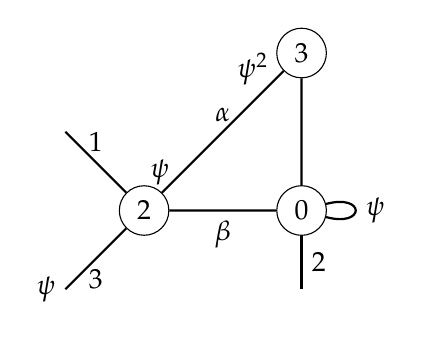
\begin{tikzpicture}[scale=1,transform shape,every loop/.style={}]
    \node[circle,draw] (A) at (0,0) {$2$};
    \node[circle,draw] (B) at (2,2) {$3$};
    \node[circle,draw] (C) at (2,0) {$0$};
    \draw[thick] (A) -- node[above]{$\alpha$} (B) -- (C) -- node[below]{$\beta$} (A);
    \draw[thick] (A) -- node[below]{$3$} (-1,-1);
    \draw[thick] (A) -- node[above]{$1$} (-1,1);
    \draw[thick] (C) -- node[right]{$2$} (2,-1);
    \draw[thick] (C) edge[loop right] node[right] {$\psi$} (C);
    \node[anchor=east] at (-1,-1) {$\psi$};
    \node[anchor=east] at (1.7,1.8) {$\psi^2$};
    \node[anchor=south] at (0.2,0.2) {$\psi$};
  \end{tikzpicture}
  \caption{$\ol{\mc{M}}_{7,3}$中的稳定图示例及其对应的陶特类。该稳定图描述态射$\ol{\mc{M}}_{2,4} \times \ol{\mc{M}}_{3,2} \times \ol{\mc{M}}_{0,5} \to \ol{\mc{M}}_{7,3}$的像。}
  \label{fig:stablegraph}
\end{figure}

CohFTs的第一类作用为平移作用。设$T \in V\ps{z}$。对CohFT $\Omega$，定义
\[ (T\Omega)_{g,n}(\bv) \coloneqq \sum_m \frac{1}{m!} p_* \Omega_{g,n+m}(\bv, T,\ldots,T) \]
当无穷级数有意义时。

\begin{exm}
若$\Omega^X$是光滑射影簇光滑射影簇 $X$的GW CohFT，且$\tau \in H^2(X)$为典范类，则无穷级数有意义，可定义$\Omega^{X,\tau}$（$X$的平移GW CohFT）。例如，若$X$为五次三维簇且$\tau = \frac{I_1}{I_0} H$，则平移至$\tau$等价于镜像映射 $q \mapsto Q(q) = q e^{\frac{I_1}{I_0}}$。
\end{exm}

第二种作用是矩阵 $R$ 的作用，如本节开头所述。设 $G_{g,n}$ 表示所有稳定图的亏格 $g$ 且具有 $n$ 条腿的集合。然后我们定义
\[ (R\Omega)_{g,n} \coloneqq \sum_{\Gamma \in G_{g,n}} \frac{1}{\ab|\Aut \Gamma|} \on{Cont}_{\Gamma}, \]
其中$\on{Cont}_{\Gamma}$由下述构造定义：
\begin{itemize}
    \item 在第 $i$ 条腿处，我们放置映射
        \[ R(-\bar{\psi}_i)^* \in \Hom(V',V) \ps{\bar{\psi}_i}; \]
    \item 在每条边上，我们放置双向量
        \[ V(\bar{\psi}_1, \bar{\psi}_2) \coloneqq \sum_{\mu} \frac{e_{\mu} \otimes e^{\mu} - R(-\bar{\psi}_1)^* e_{\mu} \otimes R(-\bar{\psi}_2)^* e^{\mu}}{\bar{\psi}_1 + \bar{\psi}_2}; \]
    \item 在每个顶点处，我们放置一个线性映射
        \[ \Omega_{g_v, n_v} \colon V^{\otimes n_v} \to H^*(\Mbar_{g_v, n_v}); \]
    \item 最后，我们考虑前推在上同调沿着态射的 $\prod_v \Mbar_{g_v, n_v} \to \Mbar_{g,n}$。
\end{itemize}

\begin{defn}
设$R$如上。则定义平移
    \[ T_R \coloneqq z (\1 - R(-z)^* \1') \in z V\ps{z}. \]
当有意义时，定义
    \[ R.\Omega \coloneqq RT\Omega. \]
\end{defn}

\begin{thm}[张怀良、郭帅、李骏 {\cite[定理~2.7]{CGL2026}}]
若系数在$\C\ps{q}$中，则
    \[ T_R \in z^2 V \ps{z} + zq V \ps{z}, \]
$R.\Omega$ 是一个良定义的 CohFT。此外，若 $\dim V = \dim V'$ 且 $\1'$ 是 $R.\Omega$ 的单位。
\end{thm}

我们稍作说明：当 $R_0 \neq \mr{Id}$ 时，翻译作用的性质。为简化，我们假设存在常数 $c$，使得 $V = V'$ 与 $R_0 \1 = c \cdot \1$ 成立。然后我们定义 $\tilde{T}_R \coloneqq z( \1 - c R(z)^{-1} \1)$，并利用稀释方程进行计算
\begin{align*}
    T_R \Omega_{g,n}(\bv) &= \sum_{m=0}^{\infty} \frac{1}{m!} p_*\Omega_{g,n+m}(\bv, T_R, \ldots, T_R) \\
    &= \sum_{k,\ell \geq 0} \frac{1}{k!\ell!} p_* \Omega_{g,n+k+\ell}(\bv, ( (1-c^{-1})\1 \cdot \psi )^{\otimes k}, ( c^{-1} \tilde{T}_R )^{\otimes \ell}) \\
    &= \sum_{k,\ell \geq 0} \frac{(1-c^{-1})^k \cdot c^{-\ell}}{\ell!} \binom{2g-2+n+k+\ell-1}{k} p_* \Omega_{g,n+\ell}(\bv, \tilde{T}_R^{\otimes \ell}) \\
    &= \sum_{m=0}^{\infty} \frac{c^{2g-2+n}}{m!} p_* \Omega_{g,n+m}(\bv, \tilde{T}_R, \ldots, \tilde{T}_R)
\end{align*}
此时成立。


\subsection{重建定理}%
\label{sub:Reconstruction theorem}

需注意，每个 CohFT 都定义了一个 Frobenius 代数。我们将 CohFT \textit{半单} 定义为：其对应的 Frobenius 代数是半单的。

\begin{thm}[Teleman {\cite{Teleman2012}}]%
\label{thm:teleman}
设 $\Omega$ 为具有平坦单位的半单 CohFT，其拓扑部分为 $\omega$。则存在唯一
    \[ R = \mr{Id} + R_1 z + \cdots \in \End(V)\ps{z} \]
满足
    \[ \Omega = R.\omega. \]
\end{thm}

\begin{exm}
回顾之前定义的 Hodge 包络 CohFT。其公式为
    \[ \Omega^{\E}_{g,n} = c(\E) = 1 + \lambda_1 + \cdots + \lambda_g. \]
    提取度为零的部分，我们发现 $\omega^{\E}$ 是一个点的 GW CohFT。利用 Mumford 的计算结果
    \[ \ch(\E) = g + \sum_{k=1}^{\infty} \frac{B_{2k}}{(2k)!}\ab(\kappa_{2k-1} + \frac{1}{2}\iota_*\sum_{i=0}^{2k-2} \bar{\psi}_1^{i} (-\bar{\psi}_2)^{2k-2-i}), \]
其中 $\kappa_{m} = p_* \bar{\psi}_{n+1}^{m+1}$、$B_{2k}$ 为 Bernoulli 数，$\iota$ 为边界包含（至多一个 $2:1$ \'etale 覆盖），公式为
    \[ c(E) = \exp \ab(-\sum_k (-1)^k (k-1)!\ch_k(E)) \]
对于任意向量丛 $E$（或直接使用量子 Riemann-Roch 定理 \footnote{），存在一个符号错误，该错误已传播至文献其他部分。} 由此可得 $R$-matrix
    \[ R(z) = \exp\ab( \sum_{k=1}^{\infty} \frac{B_{2k}}{2k(2k-1)} z^{2k-1}) = 1+\frac{1}{12}z + \cdots. \]

为验证，我们使用 $R$-matrix 计算 $\Omega_{1,1}^{\E}$。首先，考虑稳定图在 ~\Cref{fig:03graphloop} 中的情况。
    \begin{figure}[htpb]
    \begin{center}
    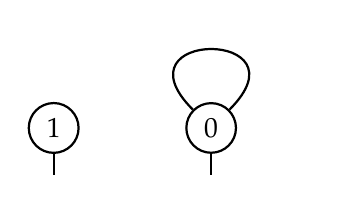
\begin{tikzpicture}[scale=1, transform shape, every loop/.style={}]
    \node[circle,draw=black,thick] (B) at (-1,0) {$1$};
    \draw[-,thick] (B) -- (-1,-0.6);
    \node[circle,draw=black,thick] (A) at (1,0) {$0$};
    \draw[-,thick] (A) -- (1,-0.6);
    \path[every node/.style={font=\sffamily\small},thick]
        (A)   edge[loop] (A);
    \end{tikzpicture}
    \end{center}
    \caption{$g=1, n=1$的稳定图}%
    \label{fig:03graphloop}
    \end{figure}
第一个图 $\Gamma_1$ 贡献为
    \begin{align*}
        \Cont_{\Gamma_1} &= T\omega_{1,1}^{\E}(R(z)^{-1}\1) \\
        &= \omega_{1,1}^{\E}(R(z)^{-1}\1) + p_* \omega_{1,1}^{\E}(R(z)^{-1}\1, T_R(z)).
    \end{align*}
使用公式 $B_2 = \frac{1}{6}$ 且已知 $\dim \Mbar_{1,1} = 1$，可得
    \[ 1 - \frac{1}{12}\psi_1 + \frac{1}{12} \kappa_1. \]
第二个图不接收尾部贡献，因为 $\dim \Mbar_{0,3} = 0$。边贡献的常数项为 $\frac{1}{12}$，考虑自同构并推向 $\Mbar_{1,1}$ 后，得到
    \[ \Cont_{\Gamma_2} = \frac{1}{12} \Delta, \]
其中 $\Delta$ 表示边界分量（含正确的叠结构）。由于本例中 $\psi_1 = \kappa_1$，故得
    \[ 1+\lambda_1 = 1 + \frac{1}{12}(\kappa_1 - \psi_1 + \Delta) = 1 + \frac{1}{12} \Delta. \]
\end{exm}




\subsection{算子形式体系与几何量子化}%
\label{sub:Operator formalism and geometric quantization}

我们将回归 Givental 的辛形式。该形式对某些计算更为便利，但本质上等同于前述内容（至少在计算生成函数时）。回顾我们曾有 Frobenius 流形结构在 $V$ 上，考虑向量空间 $\mc{V}\coloneqq V\ls{z^{-1}}$，其辛形式为
\[ (\mbf{f}(z), \mbf{g}(z)) \coloneqq \on{Res}_{z=0} \eta(\mbf{f}(-z), \mbf{g}(z)). \]
若考虑由 $\mc{V}_+ = V[z]$ 与 $\mc{V}_- = z^{-1}V\ps{z^{-1}}$ 给出的极化，则令 $\bq$ 如前（含稀释偏移），并定义 $\bp$ 为 $\mc{V}_-$ 上的坐标，使得 $(\bq, \bp)$ 构成 $\mc{V}$ 的 Darboux 坐标系。

\begin{defn}
我们将任何形式为
    \[ \mc{D} = \exp\ab(\sum_{g=0}^{\infty} \hbar^{g-1} \mc{F}_g) \]
的函数称为 \textit{ Fock 空间中的渐近元 }。
\end{defn}

给定Fock空间中的一个渐近元素，我们将通过以下公式对$\mc{V}$进行（无穷小）辛变换的量子化：
\[ \wh{p_a p_b} \coloneqq \hbar \partial_{q_a} \partial_{q_b}, \qquad \wh{p_a q_b} \coloneqq q_b \partial_{q_a}, \qquad \wh{q_a q_b} = \frac{q_a q_b}{\hbar}. \]
特别是，这将帮助我们理解如 $\hat{R} \mc{D}$ 这样的表达式。然而，我们需要谨慎处理，因为我们的公式将涉及基本解 $S_{\tau}$ 以及 $R$-矩阵，而 $S_{\tau}$ 是关于 $z^{-1}$ 的幂级数。\footnote{ 这是因为我们展开 $\frac{1}{z-\psi} = \sum_{n=0}^{\infty} \psi^n z^{-n-1}$。}

\begin{thm}[Givental {\cite{Givental2001quantization}}]
形式为$S(z^{-1}) = \mr{Id} + S_1 z^{-1} + \cdots$的算子通过以下公式作用于（渐近）Fock空间元素：
    \[ \hat{S}^{-1} \mc{D}(\bq) = e^{\frac{1}{2\hbar}W(\bq,\bq)} \mc{D}([S \bq]_+), \]
其中$W = \sum \eta(W_{mn}q_m, q_n)$由以下公式定义：
    \[ \frac{S(w^{-1})^* S(z^{-1}) - \mr{Id}}{w^{-1}+z^{-1}} = \sum \frac{W_{mn}}{w^m z^n}. \]
形式为$R(z) = \mr{Id} + R_1 z + \cdots$的算子通过以下公式作用：
    \[ \hat{R}\mc{D}(\bq) = e^{\frac{\hbar}{2} V(\partial_{\bq}, \partial_{\bq})} \mc{D}(R^{-1} \bq), \]
其中$V = \sum \eta(p_m, V_{mn} p_n)$由定义：
    \[ \frac{R(w)^* R(z) - \mr{Id}}{w+z} = \sum V_{mn} w^m z^n. \]
\end{thm}

对于半单CohFT，存在一组\textit{典范坐标} $u_{\alpha}$，使得$1$形式的$\d{u}$是代数同态$T_v V \to \C$。在半单点附近，量子连接的渐近解具有以下形式：
\[ \Psi \cdot  R \cdot e^{\frac{U}{z}}, \]
其中$\Psi$从平坦坐标切换到典范坐标，而$U = \on{diag}(u_{\alpha})$是典范坐标的矩阵。最后，定义：
\[ C = \frac{1}{2} \int^u \sum R_1^{\alpha\alpha} \d{u_{\alpha}}. \]
Teleman重构建定理的一个推论是公式：
\[ \mc{D}^X = e^{C(u)} \hat{S}^{-1}_{\tau} \hat{\Psi} \hat{R} \wh{e^{\frac{U}{z}}} \prod_{i=1}^{\dim V} \mc{D}^{\mr{pt}} \]
对于任意半单量子上同调的光滑射影簇的Gromov--Witten 理论。

\begin{exm}
作为最终示例，我们将应用Teleman定理计算任意半单CohFT的$F_1$。令$e_{\mu}$表示量子乘积的幂等基。我们将计算：
    \[ \int_{\Mbar_{1,1}} \Omega_{1,1}(e_{\beta}). \]
利用重构建定理，我们得到：
    \begin{align*}
        \int_{\Mbar_{1,1}}\Omega_{1,1}(e_{\beta}) ={}& \int_{\Mbar_{1,1}} T_R \omega_{1,1}(R(\bar{\psi})^{-1} e_{\beta}) + \frac{1}{2} T_R \omega_{0,3}(R(\bar{\psi})^{-1} e_{\beta}, V(\bar{\psi}_2, \bar{\psi}_3)) \\
        ={}& \int_{\Mbar_{1,1}}T_R\omega_{1,1}(e_{\beta}) - \int_{\Mbar_{1,1}} T_R \omega_{1,1}(R_1 e_{\beta})\bar{\psi} \\ 
        &+ \frac{1}{2}\sum_{\mu}  \omega_{0,3}(e_{\beta}, R_1 e^{\mu}, e_{\mu}) \\
        ={}& \int_{\Mbar_{1,1}} ( \omega_{1,1}(e_{\beta}) + p_* ( \omega_{1,2}(e_{\beta}, R_1 \1) \bar{\psi}_2^2 )) \\
        &- \int_{\Mbar_{1,1}} (\omega_{1,1}(R_1 e_{\beta})\bar{\psi}_1 + p_* ( \omega_{1,2}(R_1 e_{\beta}) \bar{\psi}_2^2 ) \bar{\psi}_1) \\
        &+ \frac{1}{2} \sum_{\mu} \eta(e_{\beta} \star e_{\mu}, R_1 e^{\mu}) \\
        ={}& \frac{1}{24} \sum_{\mu} ( \omega_{0,4}(e_{\mu}, e^{\mu}, e_{\beta}, R_1 \1) -\omega_{0,3}(e_{\mu}, e^{\mu}, R_1 e_{\beta}) )\\
        &+ \frac{1}{2} \eta(e_{\beta}, R_1 e^{\beta}) \\
        ={}& \frac{1}{24} \sum_{\mu}\sum_{\nu} \omega_{0,3}(e_{\mu}, e^{\mu}, e_{\nu})\omega_{0,3}(e^{\nu}, e_{\beta}, R_1 \1) \\
        &-\frac{1}{24} \sum_{\mu} \omega_{0,3}(e_{\mu}, e^{\mu}, R_1 e_{\beta}) + \frac{1}{2} (R_1)_{\beta\beta} \\
        ={}& \frac{1}{24} \ab(\eta(e^{\beta}, R_1 \1) - \sum_{\mu} \eta(e^{\mu}, R_1 e_{\beta})) + \frac{1}{2} (R_1)_{\beta\beta}.
    \end{align*}
利用恒等式：
    \begin{align*}
        \eta(R_1 \1, e^{\beta}) - \sum_{\mu} \eta(R_1 e_{\beta}, e^{\mu}) &= \sum_{\mu} \Delta_{\mu} \int_{\Mbar_{0,4}} \Omega_{0,4}(e_{\mu}, e_{\mu}, e_{\mu}, e_{\beta}) \\
        &= -\frac{1}{2}\sum_{\mu} \Delta_{\mu} \partial_{u_{\beta}} \Delta_{\mu}^{-1} \\
        &= \frac{1}{2} \sum_{\mu} \partial_{u_{\beta}} \log \Delta_{\mu},
    \end{align*}
其中$\Delta_{\mu} \coloneqq \eta(e_{\mu}, e_{\mu})^{-1}$，我们得到结果：
    \[ \int_{\Mbar_{1,1}} \Omega_{1,1}(e_{\beta}) = \frac{1}{48} \sum_{\mu} \partial_{u_{\beta}} \log \Delta_{\mu} + \frac{1}{2} (R_1)_{\beta\beta}, \]
该结果可表示为以下启发式形式：
    \[ \d{F_1^{\Omega}} = \sum_{\mu} \ab( \frac{\d{\log \Delta_{\mu}}}{48} + \frac{1}{2} (R_1)_{\mu\mu} \d{u_{\mu}} ). \]
这已知Givental所证明。
\end{exm}

\subsection{如何计算\(R\)-矩阵}%
\label{sub:How to compute the R-matrix}

我们将通过解释如何计算\(R\)-矩阵来结束本节，首先在 Frobenius 流形保形的情形下进行（例如 Gromov--Witten 理论的光滑射影簇，\(r\)-自旋曲线等）。在此例中，我们按照~\cite{PPZ2015} 考虑 3-自旋曲线的 Frobenius 流形。设\(V\)为二维，坐标为\(x\)和\(y\)，其中\(x\)对应于单位元。度量由
\[ \eta = \begin{pmatrix}
    0 & 1 \\
    1 & 0
\end{pmatrix} \]
而主要的亏格零势为\(F(x,y) = \frac{1}{2} x^2 y + \frac{1}{72} y^4\)。存在一个 \textit{Euler 向量场}
\[ E = x \pdv{}{x} + \frac{2}{3} y \pdv{}{y}, \]
它对\(\partial_x\)和\(\partial_y\)分别具有权重\(-1\)和\(-\frac{2}{3}\)。共形维度为\(\delta = \frac{1}{3}\)，我们将定义度算子：
\[ \mu(v) = [E,v] + \ab(1 - \frac{\delta}{2})v. \]
此处，\(\partial_x\)的度为\(-\frac{1}{6}\)，\(\partial_y\)的度为\(\frac{1}{6}\)。

为简化计算，我们设\(\phi = \frac{y}{3}\)并定义：
\[ \hat{\partial}_x = \phi^{1/4} \partial_x, \qquad \hat{\partial}_y = \phi^{-1/4} \partial_y, \]
然后在此框架中计算。在此设定下，量子乘法由
\[ \hat{\partial}_x \star \hat{\partial}_x = \phi^{1/4} \hat{\partial}_x, \qquad \hat{\partial}_x \star \hat{\partial}_y = \phi^{1/4} \hat{\partial}_y, \qquad \hat{\partial}_y \star \hat{\partial}_y = \phi^{1/4} \hat{\partial}_x. \]
我们需要最后一点：量子乘法由\(E\)给出
\[ E \star - = \begin{pmatrix}
    x & 2 \phi^{3/2} \\
    2 \phi^{3/2} & x 
\end{pmatrix}. \]
我们将使用递归方程计算\(R\)-矩阵\(R = 1 + R_1 z + \cdots\)
\[ [R_{k+1}, E \star -] = (k + \mu) R_k. \]
设\(R_k = \begin{psmallmatrix}
    a_k & b_k \\
    c_k & d_k
\end{psmallmatrix}\)，我们得到方程
\[ \ab[
    \begin{pmatrix}
        a_{k+1} & b_{k+1} \\
        c_{k+1} & d_{k+1}
    \end{pmatrix}, \begin{pmatrix}
        x & 2 \phi^{3/2} \\
        2 \phi^{3/2} & x 
    \end{pmatrix}
] = \frac{1}{6} \pdiagmat[empty={}]{6k-1, 6k+1} \begin{pmatrix}
    a_k & b_k \\
    c_k & d_k 
\end{pmatrix}. \]

该唯一解实际上为
\begin{align*}
    a_k &= \frac{1}{1728^k \phi^{3k/2}} \frac{1+6k}{1-6k} \frac{(6k)!}{(3k)!(2k)!} \delta_{k, \text{偶}},  \\
    b_k &= \frac{1}{1728^k \phi^{3k/2}} \frac{1+6k}{1-6k}\frac{(6k)!}{(3k)!(2k)!} \delta_{k, \text{奇}},  \\
    c_k &= \frac{1}{1728^k \phi^{3k/2}}\frac{(6k)!}{(3k)!(2k)!} \delta_{k, \text{奇}}, \\
    d_k &= \frac{1}{1728^k \phi^{3k/2}} \frac{(6k)!}{(3k)!(2k)!} \delta_{k, \text{偶}}. 
\end{align*}
如果您熟悉曲线的 tautological 关系（即模空间），您将看到系列\(a_k + b_k\)和\(c_k + d_k\)在 Faber-Zagier 关系和 Pixton 关系的表述中起作用。

在 Frobenius 流形非共形的情况下（例如在等变 Gromov--Witten 理论中），我们需要使用振荡积分或其他技术来修正\(R\)-矩阵中的初始值。以下将给出一个由 Givental~\cite{Givental2001semisimple} 给出的计算示例。在此框架下，\(X = \P^n\)成立，但该论证可推广至任意 Fano 托里克簇。回顾一下，\(\P^n\)的等变镜像对应于超势函数
\[ W = x_1 + \cdots + x_{n+1} + \sum_{i=1}^{n+1} \lambda_i \log x_i \]
(此处，为方便起见，我们改变等变参数的符号)。因此，振荡积分将呈现为
\[ I = \int_{\Gamma \subset E_q = (x_1 \cdots x_{n+1}=q)} e^{W/z} \prod_{i=1}^{n+1} \frac{\d{x_i}}{x_i}. \]
该积分被算子
\[ \prod_{i=1}^{n+1}\ab(zq \odv{}{q} -\lambda_i) - q, \]
所消解，该算子正是 Picard--Fuchs 方程，它由\(I\)-函数（在射影空间上）满足。

为展开该积分在临界点附近的表达式，我们首先需要计算临界点。此处，使用坐标\(t = \log q\)和\(T_i = \log x_i\)，我们得到方程
\[ x_i = L - \lambda_i, \]
其中\(L\)是拉格朗日乘数。这些满足方程
\[ \prod_{i=1}^{n+1} (L - \lambda_i) = q, \]
因此，对于\(\lambda\)的一般取值，在\(q = 0\)附近，拉格朗日乘子\(L_i\)的可能取值由其所属的\(\lambda_i\)决定。注意，函数\(W\)、拉格朗日乘子的取值以及因此而来的临界点，均连续依赖于\(\lambda\)，因此当\(q \neq 0\)时，在\(\lambda = 0\)处允许存在非等变极限。

当\(q = 0\)时，矩阵\(\Psi\)从平坦基的\(\ab{H^i}\)过渡到基
\[ L_i(H) = \prod_{j \neq i} \frac{H - \lambda_j}{(\lambda_i - \lambda_j)^{1/2}}, \]
其中，典范坐标的主导项可通过计算不动点（即对环面作用进行等变局部化）来得到，从而获得该拉格朗日插值。因此，我们需要在\(q = 0\)极限下计算\(L_j \ab(z q \odv{}{q}) I\)。直接计算表明，将\(L_i \ab(z q \odv{}{q})\)应用于积分会在振荡积分的被积函数中引入一个与\(\frac{q}{x_i}\)成比例的额外因子。由于我们可以重排指标，仅考虑\(i = n+1\)情形。另一项直接计算表明，除非\( j = n+1\)，否则在\(q = 0\)极限下积分为零，因此实际上可以看到\(R\)在经典极限下是对角化的。当\(j = n+1\)时，我们有
\[ \frac{q}{x_{n+1}} = x_1 \cdots x_n, \]
且积分变为
\[ \int_{\Gamma} e^{\ab( \sum_{i=1}^n x_i + (\lambda_i - \lambda_{n+1})\log x_i ) / z} \d{x_1} \cdots \d{x_n} = \prod_{i=1}^n \int_{\R} e^{x_i/z} x_i^{(\lambda_i - \lambda_{n+1})/z} \d{x_i}, \]
这仅仅是伽马函数的乘积。

\begin{lem}
我们有渐近行为
    \[ \log \Gamma(1+s) \sim s \log \ab(\frac{s}{e}) + \frac{1}{2} \log(2\pi s) + \sum_{k=1}^{\infty} \frac{B_{2k}}{2k} \frac{s^{1-2k}}{2k-1}. \]
\end{lem}
利用这一结果，我们发现，在\(q = 0\)处，\(R\)-矩阵的对角矩阵元为
\[ \log R = \sum_{k=1}^{\infty} \frac{B_{2k}}{2k} \frac{z^{2k-1}}{2k-1} \sum_{i =1}^n (\lambda_i - \lambda_{n+1})^{1-2k}. \]
根据 Givental 的结果，这意味着该\(R\)-矩阵可以恢复\(\P^n\)的等变 GW 理论，并且作为推论，由于非等变极限存在，我们得到\(\P^n\)的 Virasoro 约束。

\section{半小映射的分解定理（文学清）}%
\label{sec:Decomposition theorem for semi-small maps (文学清)}

\begin{quest}
设\(X\)为（流形，簇，解析空间等）。如何计算\(H^*(X, \C)\)？
\end{quest}

不幸的是，这个问题过于困难，因此我们将用一个新的问题来替代它。

\begin{quest}
如何利用更小的空间来检测\(H^*(X, \C)\)？
\end{quest}

\begin{thm}[K\"unneth 公式]
我们有\(H^*(X \times Y, \C) = H^*(X, \C) \otimes H^*(Y, \C)\)。
\end{thm}

不幸的是，大多数空间并非乘积，因此我们考虑以下问题。

\begin{quest}
设\(f \colon X \to Y\)为态射。能否利用\(Y\)的上同调以及\(f\)纤维的上同调来检测\(X\)的上同调？
\end{quest}

尽管这个问题仍然非常困难，但至少我们可以研究它。我们将从\(f\)为紧致流形之间的纤维丛的情况开始。答案当然是 Leray 或 Serre 谱序列，但在我们触及这一点之前，需要一些预备知识。

\begin{defn}
\(\ul{\C}_Y\)上的层是指在\(Y\)上定义的向量空间\(\mc{L}\)的局部常值\(Y\)。
\end{defn}

例如，若\(Y\)连通，则局部系统对应于\(\pi_1(Y)\)的表示。此外，若\(Y\)是代数簇，则我们需要考虑其解析化。

\begin{exm}
设\(f\)为上述纤维丛，其纤维为\(F\)。则\(R^i f_* \ul{\C}_X\)是\(Y\)上的局部系统，其纤维为\(H^i(F, \C)\)。
\end{exm}

\begin{prop}
我们有
    \[ H^*(X, \C) = H^*(X, \ul{\C}_X) = H^*(\mr{pt}, R a_{X*} \ul{\C}_X). \]
\end{prop}

\begin{thm}[Leray--Serre 谱序列]
我们有一个谱序列
    \[ E_2^{p,q} = H^p(Y, R^q f_* \ul{\C}_X) \Rightarrow H^{p+q}(X, \C). \]
\end{thm}

我们现在考虑\(f \colon X \to Y\)是两个光滑射影簇之间的光滑射影态射的情形。

\begin{thm}[Deligne {\cite{Deligne1968}}]
我们有非标准同构
    \[ R f_* \ul{\C}_X = \bigoplus_{q \geq 0} R^q f_* \ul{\C}[-q]. \]
在上同调水平上，我们有
    \[ H^*(X, \C) = \bigoplus_{q \geq 0} H^{*-q}(Y, R^q f_* \ul{\C}). \]
\end{thm}

这是射影簇的硬 Lefschetz 定理的一个推论，同时也表明 Serre 谱序列在\(E_2\)页上退化。在拓扑学中，Hopf 纤维丛会导致该现象失效。

现在设\(f \colon X \to Y\)为代数簇之间的固有态射。此时存在一个\textit{Whitney 分层}\footnote{我们明确拒绝给出它的定义。}\(Y = \bigsqcup_{\lambda} Y_{\lambda}\)，使得\(f^{-1}(Y_{\lambda}) \to Y_{\lambda}\)是\(C^{\infty}\)纤维化；其底空间可以是奇异簇。

\begin{defn}
    \(Y\)上的\(\ul{\C}_Y\)-模\(\mc{F}\)称为\textit{可构造层}，如果存在 Whitney 分层\(Y = \bigsqcup Y_{\lambda}\)，使得对每个\(\lambda\)，\(\mc{F}|_{Y_{\lambda}}\)都是局部系统。
\end{defn}

有了这一定义，可以考虑\(Y\)上的可构造层的导出范畴\(\mc{D}_c^b(Y)\)。该赋值具有六函子形式体系，其中六个函子为\(f_*, f^*, f_!, f^!, \otimes, \mc{H}\mr{om}\)，并通过下述函子满足 Verdier 对偶：
\[ D_Y \colon \mc{D}_c^b(Y) \to \mc{D}_c^b(Y). \]

\begin{defn}
    一个复形\(\mc{F}^{\bullet} \in \mc{D}_c^b(Y)\)是一个 \textit{反常层}，当且仅当它满足以下条件：
    \begin{enumerate}
        \item（支持条件）对于所有\(i\)，我们有\(\dim \on{supp} \mc{H}^{-i}(\mc{F}^{\bullet}) \leq i\)；
        \item（余支持条件）对于所有\(i\)，我们有\(\dim \on{supp} \mc{H}^{-i}(D_Y \mc{F}^{\bullet}) \leq i\)。
    \end{enumerate}
\end{defn}

\begin{rmks}\leavevmode
    \begin{enumerate}
        \item 反常层不是层，而是位于\([-\dim Y, 0]\)处的复形。
        \item 它们有两个来源。一个是交同调，另一个是黎曼–希尔伯特对应。
    \end{enumerate}
\end{rmks}

我们将需要以下事实：在\(Y\)上的反常层类\(\ms{Perv}(Y)\)是一个阿贝尔范畴，且更进一步，它是\(t\)-结构在\(\mc{D}_c^b(Y)\)上的心。特别地，对于任意\(\mc{G} \in \mc{D}_c^b (Y)\)，我们可以考虑 perverse 上同调\(^p\mc{H}^i(\mc{G}) \in \ms{Perv}(Y)\)。

\begin{thm}[Beilinson-Bernstein-Deligne-Gabber {\cite{BBD1982}}]
设\(f \colon X \to Y\)为代数簇之间的固有态射，并假设\(X\)光滑连通。\footnote{这一假设并非必要；若去掉光滑性条件，则需考虑交叉复形。}那么
    \[ R f_* \ul{\C}_X [\dim X] = \bigoplus_{i} {^p\mc{H}^i}(R f_* \ul{\C}_X)[-i]. \]
    每个\(^p\mc{H}^i (R f_* \ul{\C}_X)\)都是半单的（即每个子对象都是直和补）。
\end{thm}

\begin{defn}
设\(f \colon X \to Y\)为固有满射，且\(X\)光滑不可约。设\(Y = \bigsqcup Y_{\lambda}\)为一分层，使得\(f^{-1}(Y_{\lambda}) \to Y_{\lambda}\)是\(C^{\infty}\)-纤维化。若对所有\(y_{\lambda} \in Y_{\lambda}\)均有\(\on{codim}_Y Y_{\lambda} \geq 2 \dim f^{-1}(y_{\lambda})\)，则称\(f\)为\textit{半小映射}。等号成立时，称\(Y_{\lambda}\)为\textit{相关层}；若唯一的相关层是稠密层，则称\(f\)为\textit{小映射}。
\end{defn}

\begin{thm}[{\cite{DeCataldoMigliorini2002}}]
    若\(f \colon X \to Y\)是半小的，则\(R f_* \ul{\C}_X [\dim X]\)是\(Y\)上的反常层。
\end{thm}

\begin{proof}
    对于\(y_{\lambda} \in Y_{\lambda} \subseteq Y\)，我们有
    \[ R f_* \ul{\C}_X |_{y_{\lambda}} = \bigoplus H^i (f^{-1}(y_{\lambda}), \C). \]
    注意，当\(i > 2 \dim f^{-1}(y_{\lambda}) \leq \on{codim}_Y(Y_{\lambda})\)时，上式为零。让\(Y_{\lambda}\)遍历所有层，便得到支撑条件。由于\(f\)固有，有\(R f_* = f_!\)；再利用\(D_Y R f_* = f_! D_X\)，得到余支撑条件。
\end{proof}

\begin{exms}
    现在给出一些半小映射的例子。
    \begin{enumerate}
        \item 曲面之间任何一般有限的固有态射都是半小的。
        \item 设\(Y = \ab\{xy = t^{\ell+1}\} \subseteq \C^3\)。则存在一个消解\(f \colon \tilde{Y} \to Y\)，使得奇点得到消解，且奇点上方的纤维为一串\(\P^1\)，因此它是半小的（亦可参考前例）。
    \end{enumerate}
\end{exms}

\begin{thm}[Kaledin {\cite{Kaledin2006}}]
    一个从非奇异全纯辛簇的射影双有理态射也是半小的。
\end{thm}

\begin{exm}
    例如，Springer 消解与Grothendieck--Springer 消解均为半小映射。此外，曲面上点的 Hilbert 概形到对称积的 Hilbert--Chow 态射也是半小的。
\end{exm}

设\(f \colon X \to Y\)为半小的，并考虑分层\(Y = \bigsqcup Y_{\lambda}\)。若\(Y_{\lambda}\)相关，则
\[ \mc{L}_{\lambda} = R^{d_{\lambda}} f_* \ul{\C}_{f^{-1}(Y_{\lambda})}, \]
其中\(d_{\lambda} = 2 \dim f^{-1} (y_{\lambda})\)。则\(\mc{L}_{\lambda}\)为半单的。此处需注意，\(\mc{L}_{|\lambda} = H^{d_{\lambda}}(f^{-1}(y_{\lambda}), \C)\)。现在令\(\mr{IC}(\mc{L}_{\lambda})\)为\(\mc{L}_{\lambda}[\dim Y_{\lambda}]\)在\(\ol{Y}_{\lambda}\)上的中间延伸，其为一个反常层。

\begin{thm}[{\cite{DeCataldoMigliorini2002}}]
设\(f \colon X \to Y = \bigsqcup Y_{\lambda}\)为半小的。则存在一个典范分解
    \[ R f_* \ul{\C}_X[\dim X] = \bigoplus_{Y_{\lambda}\text{ 相关}} \mr{IC}(\mc{L}_{\lambda}). \]
\end{thm}

\begin{exm}
设\(G\)为一个约化群，其李代数为\(\g\)，并选取一个博雷尔子群\(B\)。则
    \[ G \times_B \b = \tilde{\g} \xrightarrow{\pi} \g \]
是小的。因此，我们有
    \[ R \pi_* \ul{\C}_{\tilde{\g}} [\dim \g] = \mr{IC}(\mc{L}). \]
    回顾\(\tilde{\g}^{\on{rs}} \to \g^{\on{rs}}\)是一个\(W\)-扭子空间。对于\(a \in \g^{\on{rs}}\)，我们有\(\mc{L}_{|a} \cong \C[W]\)，因此\(\mc{L} = R^0 \pi_* \ul{\C}_{\tilde{\g}^{\on{rs}}}\)。这意味着\(W\)作用于\(\mc{L}\)，且该作用可以扩展到\(\mr{IC}(\mc{L})\)和\(R \pi_* \C_{\tilde{\g}}\)，特别是对于任意\(a \in \g\)，作用于纤维\(R \pi_* \C_{\tilde{\g}}|_a\)。
\end{exm}

\begin{exm}
考虑 Springer 消解映射\(\mu \colon T^*(\on{GL}_3/B) \to \mc{N} = \mathbb{O}_{(1^3)} \sqcup \mathbb{O}_{(2,1)} \sqcup \mathbb{O}_{(3)}\)。该映射是半小的，但遗憾的是所有幂零轨道均相关。注意，上述\((2,1)\)轨道的纤维是两个\(\P^1\)在节点处粘合而成的，\((3)\)轨道的纤维是一个点，而\((1^3)\)轨道的纤维是\(\on{GL}_3/B\)。

我们看到，\(\mc{L}_{(3)}\)必须是平凡的，因为\(\mu\)在该轨道上是同构。因此，\(\mc{L}_{(2,1)} = R^2 \mu_* \ul{\C}\)是秩为 2 的\(2\)局部系统，定义在\(\mathbb{O}_{(2,1)}\)上。最后，\(\mc{L}_{(1^3)} = R^6 \mu_* \ul{\C}\)是秩为 1 的\(1\)局部系统，定义在\(\mathbb{O}_{(1^3)} = \mr{pt}\)上。因此，我们有
    \[ R \mu_* \ul{\C}_{T^*\on{GL}_3/B}[6] = \mr{IC}(\mc{L}_{(3)}) \oplus \mr{IC}(\mc{L}_{(2,1)}) \oplus \mr{IC}(\mc{L}_{(1^3)}). \]
限制到\(b \in \mathbb{O}_{(3)}\)，我们得到\(\mc{L}_{(3)} = H^0(\mr{pt})\)。限制到\(a \in \mathbb{O}_{(2,1)}\)，我们得到
    \[ H^0(X, \C) \oplus H^2(X, \C) = \mr{IC}(\mc{L}_{(3)})|_{(a)} \oplus \mr{IC}(\mc{L}_{(2,1)})|_{(a)}. \]
限制到\(0 = \mathbb{O}_{(1^3)}\)，我们得到
    \begin{align*}
        H^*(\on{GL}_3/B, \C) = \C[W] &= \mr{IC}(\mc{L}_{(3)})|_0 \oplus \mr{IC}(\mc{L}_{(2,1)})|_0 \oplus \mc{L}_{(1^3)}|_0 \\
        &= H^0(\on{GL}_3/B, \C) \oplus \ab(\text{维数为} 4) \oplus H^6(\on{GL}_3/B, \C).
    \end{align*}
作为\(W = S_3\)的表示，这些对应于平凡表示、两个标准表示的副本以及符号表示。Springer 理论中的构造与这些分解见~\cite{BorhoMacPherson1983}。
\end{exm}

\section{量子\(K\)-理论（周祐正与阎霄汉）}%
\label{sec:Quantum K-theory (阎霄汉 and 周祐正)}

\subsection{概览}%
\label{sub:Overview}

Gromov--Witten 不变量是一种在光滑射影簇\(X\)中计数曲线的方式。GW 理论产生形如
\[ \ab<\alpha_1, \ldots, \alpha_n>_{g, n, \beta} \in \Q \]
的数，其中\(\alpha_i \in H^*(X)\)为各种类，亏格为亏格\(g\)，标记点数量为\(n\)，曲线类为\(\beta \in H_2(X, \Z)\)。这已被用于研究镜像对称，且在镜像对称之外已产生双射不变量。现在，我们的目标是将整个故事提升至\(K\)-理论。量子\(K\)-理论产生数
\[ \ab<V_1, \ldots, V_n>_{g, n, \beta} \in \Z \]
对于\(V_1, \ldots, V_n \in K(X)\)，这些满足各种差分方程 \footnote{（与上同调中的微分方程类比），并在三维镜像对称和表示论中有广泛应用。}

\subsection{\(K\)-理论}%
\label{sub:K-theory}

\begin{defn}
    设\(X\)为光滑射影簇。则\(X\)的\textit{\(K\)-理论}\(K(X)\)是\(X\)上向量丛的 Grothendieck 群，并施加如下关系：若
    \[ 0 \to V_1 \to V_2 \to V_3 \to 0 \]
是短正合列，则\(V_2 = V_1 + V_3\)。
\end{defn}

\begin{rmk}\leavevmode
    \begin{enumerate}
\item \(K(X)\)是一个具有直和与张量积运算的环；
\item 的 Chern 特征标给出同构\(K(X) \to A^*(X)\)，至少在\(\Q\)上成立。
    \end{enumerate}
\end{rmk}

\begin{exm}
设\(X = \P^n\)，且定义\(P = \mc{O}(-1)\)。则有
    \[ K(X) = \C[P^{\pm 1}]/(P-1)^{n+1} \xrightarrow{\on{ch}} A^*(X) = \C[H]/H^{n+1}. \]
\end{exm}

对于一个不假设为光滑的 Deligne--Mumford 叠，存在两种版本
\[ K_0(X) \supset K^0(X), \]
其中\(K_0\)表示凝聚层，\(K^0\)表示完美复形。它们在光滑的射影簇上一致，因此从现在起\(K(X)\)将表示\(K_0(X)\)。存在张量积
\[ K^0(X) \otimes K_0(X) \to K_0(X) \]
和一个前推
\[ f_* \colon K(X) \to K(Y) \qquad V \mapsto \sum (-1)^i R^i f_* V \]
沿固有态射。若\(f\)是一个完美态射（例如平坦态射或正则嵌入），则存在拉回
\[ f^* \colon K(Y) \to K(X) \qquad W \mapsto \sum (-1)^i \on{Tor}_i^{f^{-1} \mc{O}_Y} (\mc{O}_X, f^{-1} W). \]

\subsection{曲线的模空间}%
\label{sub:Moduli of curves}

回忆模空间
\[ \bar{M}_{g,n}(X, \beta) = \ab\{ f \colon (\Sigma, p_1, \ldots, p_n) \to X \mid g(\Sigma) = g, f_*[\Sigma] = \beta, \abs{\Aut f} < \infty \} \]
到\(X\)的稳定映射。其存在评估映射
\[ \ev_i \colon \bar{M}_{g,n}(X, \beta) \to X \qquad (f, \Sigma, \ul{p}) \mapsto f(p_i). \]
还有通用切向量线\(L_i = \sigma_i^* \omega_{ \mc{C}/\bar{M} }\)。

该模空间是具有完美障碍理论的固有 DM 叠，因而产生虚拟结构层\(\mc{O}^{\vir}_{g,n,\beta}\)。它来自\textit{虚拟切丛}的结构，其中
\[ \mathbb{T}_{(f, \Sigma, \ul{p})} \bar{M}_{g,n}(X, \beta) = \chi(\Sigma, f^* T_X) - \chi(\Sigma, T_{\Sigma}(-p_1 - \cdots - p_n)). \]
粗略地说，若\(\bar{M}\)是向量丛\(E\)在簇\(Y\)上一个截面的零点，则\(\mc{O}^{\vir} = \mc{O}_Y \otimes \mr{Eu}(E)\)，其中 K-理论欧拉类为\(\mr{Eu}(E) = \sum (-1)^i \Lambda^i E^{\vee}\)。

\subsection{Gromov--Witten 不变量}%
\label{sub:KGW invariants}

量子\(K\)-理论见~\cite{Lee2004}，置换等变理论见~\cite{Givental2017K1,GiventalK7}。下面使用的 Deligne--Mumford 叠的 Riemann--Roch 公式由 To\"en~\cite{Toen1999} 证明。

\begin{defn}
K-理论 GW 不变量由
    \[ \ab<V_1, \ldots, V_n>_{g,n,\beta} \coloneqq \chi\ab(\bar{M}_{g,n}(X, \beta); \mc{O}^{\vir} \otimes \bigotimes_{i=1}^n \ev_i^* V_i). \]
\end{defn}

若\(V_1, \ldots, V_n\)是实际的向量丛，则该不变量为整数，但通常我们考虑在特征为零的域上的\(K_0\)。我们也可以定义引力下降项
\[ \ab<V_1 L_1^{k_1}, \ldots, V_n L_n^{k_n}>_{g,n,\beta} \coloneqq \chi\ab(\bar{M}_{g,n}(X, \beta); \mc{O}^{\vir} \otimes \bigotimes_{i=1}^n ( \ev_i^* V_i )L_i^{k_i} ). \]
通过在\(\bar{M}_{g,n}(X, \beta)\)上对标记点进行置换的\(S_n\)作用，对象\(\bigotimes_{i=1}^n \ev_i^* V\)和\(\bigotimes_{i=1}^n L_i^k\)是\(S_n\)-等变。

\begin{defn}
    我们定义 \textit{置换不变的 K-理论 GW 不变量} 为
    \begin{align*}
        \ab<V L_1^k, \ldots, V L_n^k>_{g,n,\beta}^{S_n} &\coloneqq \chi\ab([ \bar{M}_{g,n}(X, \beta)/S_n ]; \mc{O}^{\vir} \otimes \bigotimes_{i=1}^n ( \ev_i^* V ) L_i^k) \\
        &= \dim \chi_{S_n} \ab(\bar{M}_{g,n}(X, \beta); \mc{O}^{\vir} \otimes \bigotimes_{i=1}^n ( \ev_i^* V ) L_i^k )^{S_n}.
    \end{align*}
\end{defn}

给定\(t(q) = \sum_{n \in \Z} t_n q^n \in K(X)[q,q^{-1}]\)，我们可以定义
\[ \ab< t(L_1), \ldots, t(L_n)>^{S_n}_{g,n,\beta} \coloneqq \chi ([\bar{M}_{g,n}(X,\beta)/S_n], \cdots). \]
更一般地，若\(H = S_{a_1} \times \cdots \times S_{a_m} \subset S_n\)，我们可以定义
\[ \ab<t_1(L_1), \ldots, t_1(L_{a_1}), t_2(L_{a_1+1}), \ldots, t_2(L_{a_1+a_2}), \ldots>_{g,n,\beta}^H. \]

\begin{rmk}
我们希望讨论与普通 GW 不变量的一些关系。回忆 Hirzebruch-Riemann-Roch 定理表明：
    \[ \chi(M; V) = \int_M \on{ch}(V) \on{td}(T_M). \]
当\(M\)是一个光滑 DM 叠时，T\"oen 证明了该公式
    \[ \chi(M; V) = \int_{IM} \wt{\on{ch}}(V) \wt{\on{td}}(T_M), \]
其中\(IM = M \times_{\Delta, M \times M, \Delta} M\)是\(M\)的惯性叠，波浪线表示取 orbifold 的 Chern 特征标和 Todd 类。
\end{rmk}

\begin{exm}
若\(M = B\mu_r\)，则\(IM = \bigsqcup_{g \in \mu_r} B \mu_r\)。若\(M = \P(1, r)\)是一个加权\(\P^1\)，则\(IM = M \sqcup \bigsqcup_{g \neq 1 \in \mu_r} B\mu_r\)。
\end{exm}

\begin{exm}
设\(M = BG\)为有限阿贝尔群\(G\)的概形，且\(V\)是\(BG\)上的向量丛，即\(G\)的表示。则有\(\chi(M, V) = \dim V^G\)。另一方面，我们有
    \[ \int_{IM} \wt{\on{ch}}(V) \cdot \wt{\on{td}}(T_M) = \int_{IM} \on{tr}_g V = \sum_{g \in G} \frac{1}{\abs{G}} \on{tr}_g V = \dim V^G, \]
因此，我们在此设定下已验证了 Riemann-Roch 公式。
\end{exm}

\subsection{公理性质}%
\label{sub:Axiomatic properties}

\begin{lem}[{\cite{GiventalK7}}]
我们有 \textit{ 字符串方程}
    \begin{align*}
        \ab< 1, x_1(L), \ldots, x_k(L), t, \ldots, t >_{g, 1+k+n, \beta}^{S_n} = \ab<x_1(L), \ldots, x_k(L), t^{\otimes n}>^{S_n}_{g,k+n,\beta} \\
        + \sum_i \ab< \cdots, \frac{x_i(L) - x_i(1)}{L-1}, \ldots, t^{\otimes n}>^{S_n}_{g,k+n,\beta}. 
    \end{align*}
\end{lem}

\begin{proof}
证明与 GW 理论中的情况相同，来源于沿映射\(\pi \colon\bar{M}_{g,n+1}(X,\beta) \to \bar{M}_{g,n}(X,\beta)\)计算\(\pi^* L_i\)。
\end{proof}

\begin{lem}[{\cite{GiventalK7}}]
我们有 \textit{ 淡化方程}
    \begin{align*}
        \ab<L-1, x_1(L), \ldots, x_k(L), t^{\otimes n}>_{g,1+k+n,\beta}^{S_n} ={}& (k-2)\ab<x_1(L), \ldots, x_k(L), t^{\otimes n}>_{g,k+n,\beta}^{S_n} \\
        &+ \ab<x_1(L), \ldots, x_k(L), t, t^{\otimes n-1}>_{g,k+n,\beta}^{S_{n-1}}.
    \end{align*}
\end{lem}

\begin{proof}
我们利用以下事实
    \[ \pi_* L = k + \on{Ind}_{S_{n-1}}^{S_n}(1) - 1, \]
其中\(\pi\)忽略第一个标记点，而\(L = \omega_{\pi} (p_1 + \cdots + p_n)\)。这源于存在一个留数映射这一事实。
    \[ H^0(L) \xrightarrow{\on{Res}} \bigoplus_{i=1}^{k+n} \C p_i \xrightarrow{\sum} \C. \]
中间项是\(k\)的平凡表示的直和以及一个标准表示。
\end{proof}

\begin{notn}
固定\(\tau, t \in K(X)\)。我们将表示为
    \[ \ab<\!\ab<x_1(L_1), \ldots, x_k(L_k)>\!>_{g,k} \coloneqq \sum_{m,n,\beta} \frac{Q^{\beta}}{m!} \ab<x_1(L_1), \ldots, x_k(L_k), \tau^{\otimes m}, t^{\otimes n}>_{g,k+m+n,\beta}^{S_n}. \]
我们令\(\{\phi_{\alpha}\}\)为\(K(X)\)的一组基，\(\{\phi^{\alpha}\}\)为其对偶基。然后定义配对
    \[ g_{\alpha\beta} = \chi(X, \phi_{\alpha} \otimes \phi_{\beta}). \]
该配对并非完全正确，因此我们考虑
    \[ G_{\alpha\beta} = g_{\alpha\beta} + \ab<\!\ab<\alpha,\beta>\!>_{0,2}. \]
我们令\(g^{\alpha\beta} = (g_{\alpha\beta})^{-1}\)和\(G^{\alpha\beta} = (G_{\alpha\beta})^{-1}\)。
\end{notn}

\begin{lem}[{\cite{Givental2000K}}]
给定\(A,B,C,D \in K(X)[q,q^{-1}]\)，我们有 \textit{WDVV 方程}
    \begin{align*}
        \sum_{\alpha,\beta} \ab<\!\ab< A(L), B(L), \phi_{\alpha}>\! >_{0,3}& G^{\alpha\beta}\ab<\!\ab< C(L), D(L), \phi_{\beta}>\! >_{0,3} \\
        &= \sum_{\alpha,\beta} \ab<\!\ab< A(L), C(L), \phi_{\alpha}>\! >_{0,3} G^{\alpha\beta}\ab<\!\ab< B(L), D(L), \phi_{\beta}>\! >_{0,3}. 
    \end{align*}
\end{lem}

\begin{proof}
将\(\bar{M}_{0,4} = \P^1\)上边界分量的等式拉回。在\(K\)-理论中，当将\(\mc{O}_D\)与\(\mc{O}_{C_i}\)关联时，若\(D = \bigcup C_i\)，则需应用包含-排斥原理，这导致了\(G^{\alpha\beta}\)的出现。
\end{proof}

\subsection{环空间形式体系}%
\label{sub:Loop space formalism}

\begin{defn}
\textit{ 环路空间 } \((\mc{K}, \Omega)\)由 "
    \[ \mc{K} = K(X)(q) \ps{Q}\]
带辛形式
    \[ \Omega(f, g) = - \on{Res}_{q = 0, \infty} \ab<f(q^{-1}), g(q)>_X \frac{\d{q}}{q}. \]
\end{defn}

\begin{rmk}
存在一个极化\(\mc{K} = \mc{K}_+ \oplus \mc{K}_-\)，其中
    \[ \mc{K}_+ = K(X)[q, q^{-1}]\ps{Q} \]
    且
    \[ \mc{K}_- = \ab\{ \frac{f}{g} \mid f, g \in K(X)\ps{Q}[q], g(0) \neq 0, \deg f < \deg g\}. \]
例如，\(\frac{1}{1-q} \in \mc{K}_-\)。
\end{rmk}

\begin{defn}
    \textit{大\(J\)-函数} \(J \colon \mc{K}_+ \to \mc{K}\)由
    \[ \mathbf{t} = \mathbf{t}(q) \mapsto 1 - q + \mathbf{t}(q) + \sum_{\beta, \alpha} Q^{\beta} \phi^{\alpha} \ab< \frac{\phi_{\alpha}}{1-qL}, \mathbf{t}(L)^{\otimes n}>_{0, 1+n, \beta}^{S_n}. \]
\end{defn}

\begin{rmk}
注意，应用 Riemann-Roch 后，我们有
    \begin{align*}
        \chi\ab([\bar{M}/S_n], \frac{1}{1-qL}) &= \int_{I[\bar{M}/S_n]} \on{ch}\ab(\frac{1}{1-qL}) \on{td}.
    \end{align*}
每一项均化为形式\(\on{ch}\ab(\on{tr}_g \frac{1}{1-qL})\)，从而得到形式\(\on{ch}\ab(\frac{1}{1-q\zeta L})\)，其中单位根\(\zeta\)为某个根。随后我们展开
    \[ \frac{1}{1-q\zeta L} = \frac{1}{(1-q \zeta) - q\zeta (L-1)} = \sum_k \frac{(q\zeta)^k}{(1-q\zeta)^{k+1}}(L-1)^k. \]
\end{rmk}

\begin{defn}
\textit{ 生成元锥 } 定义为\(\mc{L} \coloneqq \Ima J \subset \mc{K}\)，其中我们考虑在\(1-q\)处的\(Q\)-adic 本征拓扑的邻域。
\end{defn}

\begin{exm}
令\(X = \P^n\)。则我们有
    \[ J(0) = (1-q) \sum_{d \geq 0} \frac{Q^d}{\prod_{\ell=1}^d (1-Pq^{\ell})^{n+1}}, \]
其中\(P = \mc{O}(-1)\)。如前所述，可展开
    \[ \frac{1}{1-P q^{\ell}} = \frac{1}{(1-q^{\ell}) - q^{\ell}(P-1)} = \sum_{k=0}^{\infty} \frac{q^{\ell k}}{(1-q^{\ell})^{k+1}}(P-1)^k. \]
\end{exm}

\begin{prop}[{\cite{GiventalK7}}]
事实上，\(\mc{L}\)实际上是\(\mc{K}\)中的一个锥，且有
    \[ \mc{L} = \bigcup_{t \in K(X)\ps{Q}} (1-q) S_{t}^{-1}(q) \mc{K}_+. \]
\end{prop}

我们亦可引入一个「巨大的」\(J\)-函数
\[ J(\mathbf{t}, \tau) = 1-q + \mathbf{t}(q) + \tau + \sum_{\beta, k, \alpha} \frac{Q^{\beta}}{k!} \phi^{\alpha} \ab< \frac{\phi_{\alpha}}{1-qL}, \mathbf{t}(L)^{\otimes n}, \tau^{\otimes k}>_{0,1+n+k,\beta}^{S_n}. \]
若固定\(\mathbf{t}(q)\)，则\(J(\tau)\)是 \textit{ 上关于 } 的微分方程在 Frobenius 流形（即\(\tau\)）中的基本解。此外，\(\mc{L}^{\mathbf{t}}=  \Ima J(\tau)\)实际上是一个 Lagrangian 锥。

\begin{exm}
考虑由 Adams 运算给出的\(f \colon \C[\Lambda_1^{\pm}, \Lambda_2^{\pm}] \to \C[\Lambda_1^{\pm}, \Lambda_2^{\pm}]\)
    \[ t \mapsto \on{tr}_{(1\cdots n)} t^{\otimes n} = \Psi^n (t). \]
因此，该映射将\(\Lambda_1 \mapsto \Lambda_1^n\)和\(\Lambda_2 \mapsto \Lambda_2^n\)映射到。然而，在\(t\)中求导并不明确，因为我们可能需要\(nv t^{n-1} = \Psi^n(v)\)，因此\(J\)-函数不满足\(\mathbf{t}\)中的量子微分方程。
\end{exm}

\subsection{等变\(K\)-理论与局部化}%
\label{sub:Equivariant K-theory and localization}

不动点递推与射影空间的计算见~\cite{GiventalK2}。

令一个环面\(T = (\C^{\times})^r\)作用于一个光滑的射影簇\(X\)。

\begin{defn}
\textit{等变\(K\)-理论} \(K_T(X)\)是\(T\)-等变向量丛在\(X\)上的 Grothendieck 群。
\end{defn}

\begin{exm}
例如，我们有
    \[ K_T(\on{pt}) = \on{Rep}(T) = \C[\Lambda_1^{\pm}, \ldots, \Lambda_r^{\pm}], \]
其中\(\Lambda_i\)是具有权重\((0, \ldots, 1, \ldots, 0)\)的\(1\)维表示。
\end{exm}

\begin{rmk}
对于任意\(X\)，\(K_T(X)\)是\(K_T(\mr{pt})\)-代数。
\end{rmk}

\begin{exm}
考虑\(\P^n\)的完全等变\(K\)-理论。则有
    \[ K_T(\P^n) = \C[P^{\pm}, \Lambda_0^{\pm}, \ldots, \Lambda_n^{\pm}] \big/ \prod_{i=0}^n (P-\Lambda_i). \]
当我们将\(\Lambda_i = 1\)专门化时，我们得到非等变\(K\)-理论。
\end{exm}

\begin{defn}
我们可以定义等变 Euler 示性数为前推
    \[ \chi_T = \pi_* \colon K_T(X) \to K_T(\mr{pt}). \]
\end{defn}

\begin{exm}
例如，我们有\(\chi_T(\mc{O}_{\P^1}(1)) = \Lambda_0^{-1} + \Lambda_1^{-1}\)。类似地，我们有
    \[ \chi_T(\mc{O}(2)) = \Lambda_0^{-2} + \Lambda_0^{-1} \Lambda_1^{-1} + \Lambda_1^{-2}. \]
\end{exm}

\begin{notn}
注意\(\on{Frac}(T) = \on{Frac}(\on{Rep}(T))\)。然后我们将设定
    \[ K_T^{\loc}(X) \coloneqq \on{Frac}(T) \otimes_{\on{Rep}(T)} K_T(X). \]
\end{notn}

我们需要以下事实。令\(F\)为\(T\)在\(X\)上的不动点集合，并考虑\(\iota \colon F \hookrightarrow X\)。则存在一个\(\on{Frac}(T)\)-代数同构
\[ K_T^{\loc}(X) \xrightarrow{\iota^*} K_T^{\loc}(F). \]

\begin{rmk}
逆映射由
    \[ (\iota^*)^{-1} = \bigoplus_{i=1}^r \frac{\iota_{i*}}{\on{Eu}(N_{F_i/X})}, \]
给出，其中\(\on{Eu}(V) \coloneqq \sum_{j = 0}^{\on{rk} V} (-1)^j \Lambda^j V^*\)是 K-理论欧拉类。
\end{rmk}

\begin{exm}
在\(\P^n\)上，我们有\(n+1\)个孤立的不动点\(F_i\)，然后我们得到
    \[ \frac{\iota_{i*} \mc{O}_{F_i}}{\on{Eu}(N_{F_i/\P^n})} = \prod_{j \neq i} \frac{P - \Lambda_j}{\Lambda_i - \Lambda_j}. \]
这些是\(K_T^{\loc}(\P^n)\)的幂等元。
\end{exm}

利用等变局部化，我们得到
\[ \chi_T(X; V) = \sum_i \chi\ab(F_i; \frac{\iota_i^* V}{\on{Eu}(N_{F_i/X})}). \]

\begin{rmk}
在\(\Lambda = 1\)极限下，我们可以得到非等变 Euler 示性数。
\end{rmk}

\begin{exm}
令\(X = \P^1\)。则我们计算
    \begin{align*}
        \chi_T(\P^1, \mc{O}(1)) &= \chi\ab(F_0, \frac{\mc{O}(1)|_{F_0}}{\on{Eu}(T_{F_0/\P^1})}) + \chi\ab(F_1, \frac{\mc{O}(1)|_{F_1}}{\on{Eu}(T_{F_1/\P^1})}) \\
        &= \frac{\Lambda_0^{-1}}{1 - \frac{\Lambda_0}{\Lambda_1}} + \frac{\Lambda_1^{-1}}{1 - \frac{\Lambda_1}{\Lambda_0}} \\
        &= \Lambda_0^{-1} + \Lambda_1^{-1}. 
    \end{align*}
\end{exm}

自此，我们假设\(X\)是一个 GKM 流形。我们的目标是利用局部化作用于\(\bar{M}_{g,n}(X, \beta)\)，以研究\(X\)的大\(J\)-函数。任何\(T\)-不动的稳定映射\(f \colon (\Sigma, \ul{p}) \to X\)具有两类不可约分支：一类完全映射到不动点，另一类则通过\(1\)维轨道的分支覆叠映射。遗憾的是，我们无法通过虚拟局部化计算大\(J\)-函数，但仍可对其进行研究。

令\(f = f(q) \in \mc{K} = K_T^{\loc}(X)(q)\ps{Q}\)。将不动点记为\(F_{\alpha}\)，其中\(\alpha = 1, \ldots, r\)通过包含映射\(\iota_{\alpha} \colon F_{\alpha} \hookrightarrow X\)。然后记
\[ f_{\alpha}(q) = \iota_{\alpha}^* f(q) \in K_T^{\loc}(\on{pt})(q)\ps{Q}. \]
则\(f \in \mc{L}\)当且仅当对所有\(\alpha\)，以下条件成立：
\begin{enumerate}
    \item 给定\(\lambda \in T_{F_{\alpha}} X\)且\(m \in \N_+\)，\(f_{\alpha}(q)\)在\(q = \lambda^{1/m}\)处至多有单极点，且
        \[ \on{Res}_{q = \lambda^{1/m}} f_{\alpha}(q) \frac{\d{q}}{q} = -\frac{Q^m}{m} \cdot \frac{\on{Eu}(T_{F_{\alpha}/X})}{\on{Eu}(T^{\vir}_{\phi_{\alpha,\alpha',m}}\bar{M}_{0,2}(X, m \cdot \beta(\alpha, \alpha')))} \cdot f_{\alpha'}(\lambda^{1/m}). \]
        这里，\(\lambda \in T_{F_{\alpha}}X\)表示\(\lambda\)是\(1\)维的\(T_{F_{\alpha}} X\)的子表示。此外，\(\beta(\alpha,\alpha')\)是由权重\(\lambda\)决定的\(T\)的\(1\)维轨迹的度，而\(\phi_{\alpha, \alpha', m}\)参数化了该\(1\)维轨迹的\(m:1\)重覆盖。
    \item \(f_{\alpha}(q)\)在\(0, \infty\)处有其他极点，且在根的单位处有极点，其余地方则为正则。此外，还存在各种次要条件。
\end{enumerate}

\begin{exm}
    令\(X = \P^n\)。则
    \[ J_T^X(0) = (1-q) \sum_{d \geq 0} \frac{Q^d}{\prod_{i=0}^n \prod_{\ell = 1}^d \ab(1 - \frac{P}{\Lambda_i} q^{\ell})} \in K_T(X)(q) \ps{Q}. \]
    这则意味着
    \[ J_T^X(0) |_{F_j} = (1-q) \sum_{d \geq 0} \frac{Q^d}{\prod_{i=0}^n \prod_{\ell = 1}^d \ab(1 - \frac{\Lambda_j}{\Lambda_i}q^{\ell})}, \]
    因此极点位于\(q = \ab(\frac{\Lambda_i}{\Lambda_j})^{1/\ell}\)。此外，注意
    \[ T_{F_j} X = \frac{\Lambda_0}{\Lambda_j} + \cdots + \frac{\Lambda_n}{\Lambda_j} - 1. \]
\end{exm}

\subsection{量子 K/GV 对应关系}%
\label{sub:Quantum K/GV correspondence}

五次三维簇的对应关系由~\cite{GaroufalidisScheidegger2022} 猜想，并由~\cite{ChouLeeQuintic} 证明。下面的 Calabi--Yau 三维簇公式由 Chou--Lee~\cite{ChouLee2025} 给出。

我们的目标是计算\(J^K(0)\)，其中 Calabi--Yau 三维簇为 Calabi-Yau 三维流形。该结果由 Jockers-Mayr 和 Garoufalidis-Scheidegger 猜测。

\begin{thm}[{\cite{ChouLee2025}}]
    我们有
    \begin{align*}
        J^K(0) &\coloneqq (1-q) + \sum_{\beta, \alpha} Q^{\beta} \Phi^{\alpha} \ab<\frac{\Phi_{\alpha}}{1-qL}>_{0,1,\beta}^{X,K} \\
        &= (1-q) + \sum_{\beta} \sum_{r=1}^{\infty} \mr{GV}_{\beta} Q^{r\beta} \ab[\sum_{j=1}^{n_1} \Phi^{1j} a(r, q^r) + \Phi^{01} b(r, q^r)],
    \end{align*}
    其中\(\ab\{\Phi_{\alpha}\}_{\alpha=1}^N\)是\(K^0(X)\)的一组基，其分解满足
    \[ \ab\{\Phi_{\alpha}\}_{\alpha=1}^N = \bigsqcup_{i=0}^3 \ab\{\Phi_{ij}\}_{j=1}^{n_i} \]
    使得固定\(i\)的集合\(\ch(\Phi_{ij})\)构成\(H^{2i}(X)\)的一组基。然后我们选择对偶基\(\ab\{\Phi^{\alpha}\}_{\alpha} = \ab\{\Phi^{ij}\}_{i,j}\)。此外，我们设定多重覆盖公式
    \begin{align*}
        a(r, q^r) &= \frac{r-1}{1-q^r} + \frac{1}{(1-q^r)^2}, \\
        b(r, q^r) &= \frac{r^2-1}{1-q^r} + \frac{3}{(1-q^r)^2} - \frac{2}{(1-q^r)^3}.
    \end{align*}
    最后，GV 表示 Gopakumar-Vafa 不变量，其在亏格零中定义为
    \[ \mr{GW}_{0,\beta} = \sum_{r \mid \beta} \frac{1}{r^3} \mr{GV}_{\beta/r}. \]
    通过 M\"obius 反转，我们得到
    \[ \mr{GV}_{\beta} = \sum_{r \mid \beta} \frac{\mu(r)}{r^3} \mr{GW}_{0,\beta/r}. \]
\end{thm}

\begin{cor}[{\cite{ChouLee2025}}]
    我们有
    \[ \ab<1>_{0,1,\beta}^K = \sum_{r \mid \beta} r^2 \mr{GV}_{\beta/r}. \]
    应用 M\"obius 反转，我们得到 \footnote{注意，该结果在所有亏格中由 Ionel--Parker~\cite{IonelParker2018} 获得。}
    \[ \mr{GV}_{\beta} = \sum_{r \mid \beta} r^2 \mu(r) \ab<1>_{0,1,\beta/r}^K \in \Z. \]
    此外，我们可以通过\footnote{恢复常规的 Gromov--Witten 不变量。这类似于将 Hirzebruch-Riemann-Roch 应用于计算 K-理论配对，其中最高次度项仅观察到两个输入的 Chern 字符。}
    \[ \lim_{q \to 1} (1-q)^3 \ab<\frac{1}{1-qL}>_{0,1,\beta}^{X,K} = \sum_{r \mid \beta} \frac{-2}{r^3} \mr{GV}_{\beta/r} = -2 \mr{GW}_{\beta} = \ab<\psi>_{0,1,\beta}^{\mr{GW}}. \]
\end{cor}

粗略地说，我们可以将\(J^K(0) \in \Z\ps{q}\ps{Q}\)视为，但为了更精确，我们可以考虑
\[ J^K(0) \in 1-q + \mc{K}_-. \]
    这里，我们展开\(\frac{1}{1-qL} = \sum q^i L^i\)。
    我们还需要考虑，若\(M\)是一个 DM 叠，且\(L\)是\(M\)上的线丛，则该函数
\[ f^{\Phi}(q) \coloneqq \chi\ab(M, \frac{\Phi}{1-qL}) \in \Z \ps{q} \]
对于\(\abs{q} < \ep\)收敛到一个有理函数。注意，极点仅出现在单位根处。

该事实可通过轨道Riemann-Roch定理证明。将惯性分解为
\begin{align*}
    IM &= \bigsqcup_{i \in I} M_i \\
    &= \bigsqcup_{\zeta} M_{\zeta},
\end{align*}
其中\(M_{\zeta}\)是满足\(g\)作用于\(L\)且特征值为\(\zeta\)的扭曲子空间的并集。利用此，我们可计算
\begin{align*}
    \chi\ab(M, \frac{1}{1-qL}) &= \sum_{i \in I} \int_{M_i} \on{td}(M_i) \on{ch} \ab(\frac{ \on{Tr}_g \ab(\frac{1}{1-qL}) }{\lambda_{-1}(N_{M_i/M}^*)}) \\
    &= \sum_{\zeta} \int_{M_{\zeta}} \on{td}(M_{\zeta}) \sum_{k \geq 0} \frac{(\zeta q)^k}{(1-\zeta q)^{k+1}} \frac{( \on{ch}(L)-1 )^k}{\ch \lambda_{-1}(N^*)},
\end{align*}
因此，所有极点必在单位根处。此处，我们使用展开式
\[ \frac{1}{1-\zeta q L} = \sum_{k \geq 0} \frac{(\zeta q)^k}{(1-\zeta q)^{k+1}} (L-1)^k \]
并取 Chern 特征标。

\begin{exm}
设\(L = \mc{O}(1)\)作用于\(\P^1\)。则有
    \begin{align*}
        \chi\ab(\P^1, \frac{1}{1-qL}) &= \chi\ab(\P^1, \frac{1}{1-q} + \frac{q}{(1-q)^2}(L-1)) \\
        &= \sum_{i \geq 0} q^i (i+1) \\
        &= \frac{1}{(1-q)^2}.
    \end{align*}
\end{exm}

\begin{exm}
我们将考虑加权射影空间。则有
    \begin{align*}
        \chi\ab(\P(w_0, \ldots, w_n), \frac{1}{1-qL}) &= \prod_{i=0}^n \frac{1}{1-q^{w_i}}. 
    \end{align*}
\end{exm}

\subsection{阿代尔刻画}%
\label{sub:Adelic characterization}

需回忆，GW与GV不变量之间存在一种关系，该关系在所有亏格中可通过显式公式表达。另一方面，我们可通过\(q \to 1\)极限从 KGW 不变量中恢复 GW 不变量。在另一方向上，我们需要 Givental--Tonita 的 \textit{阿代尔刻画}~\cite{GiventalTonita2014}。其思想是，若存在有理函数\(f\)，则可通过在单位根处的 Laurent 展开式恢复该函数。
\[ f_{q=\zeta} = \sum f_{\zeta, k} (1-\zeta^{-1} q)^k \]
在单位根\(\zeta\)处的展开式。

我们将研究惯性叠\(I\bar{M}_{0,1}(X, \beta)\)。其组成部分可通过 ~\Cref{fig:givental-png} 或 ~\Cref{fig:adelic-components} 追踪。
\begin{figure}[htpb]
    \centering
    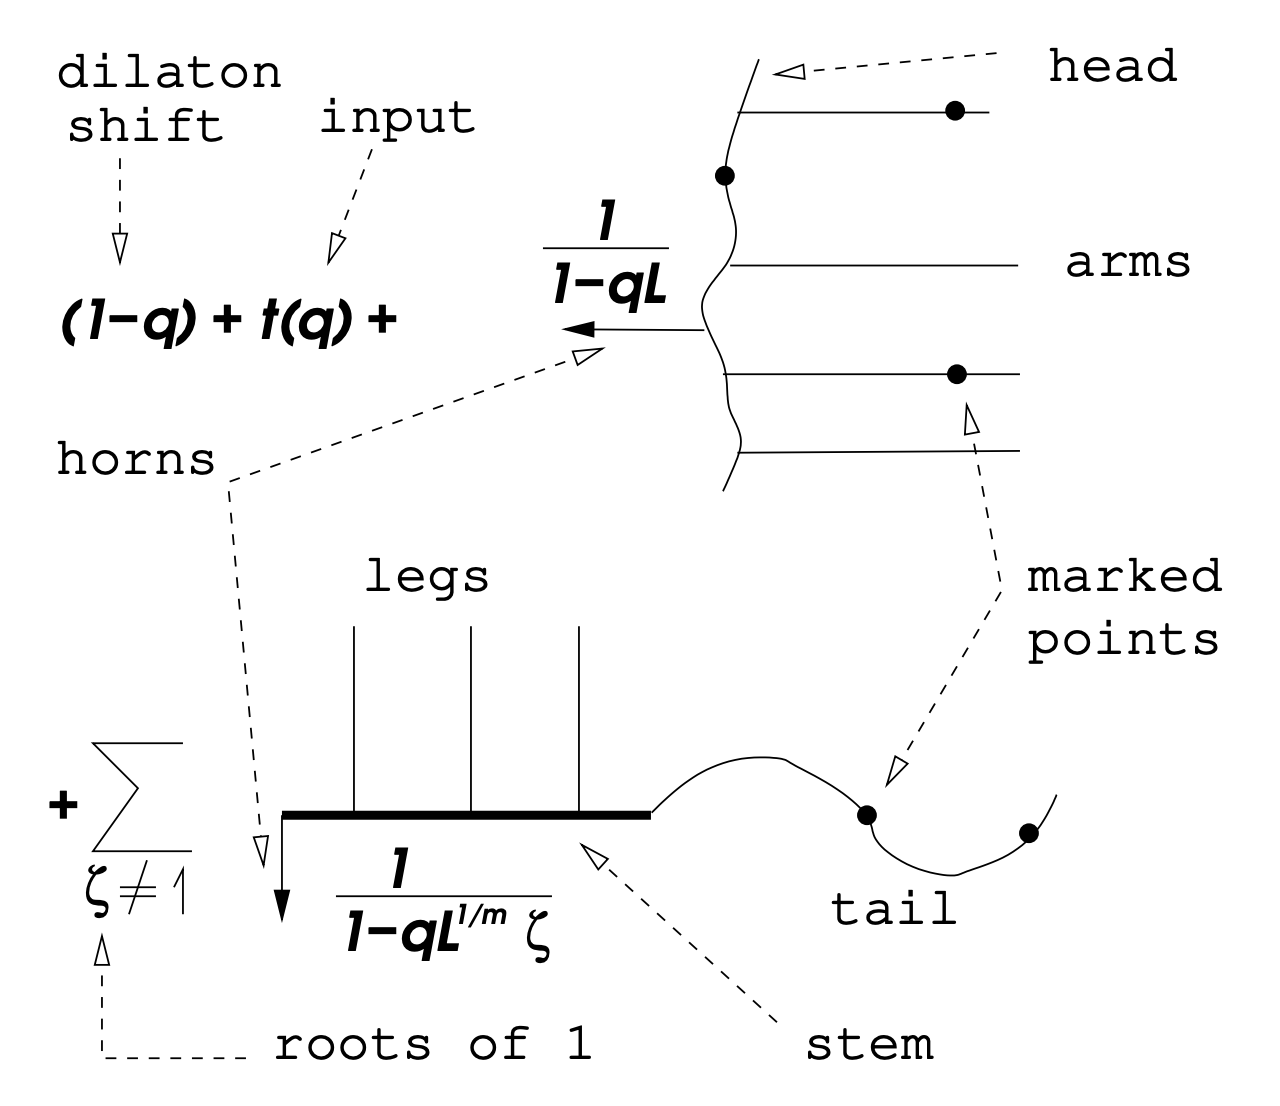
\includegraphics[width=0.8\textwidth]{givental.png}
\caption{一种追踪 Givental--Tonita 惯性分量的方法}
    \label{fig:givental-png}
\end{figure}

\begin{figure}[htpb]
    \centering
    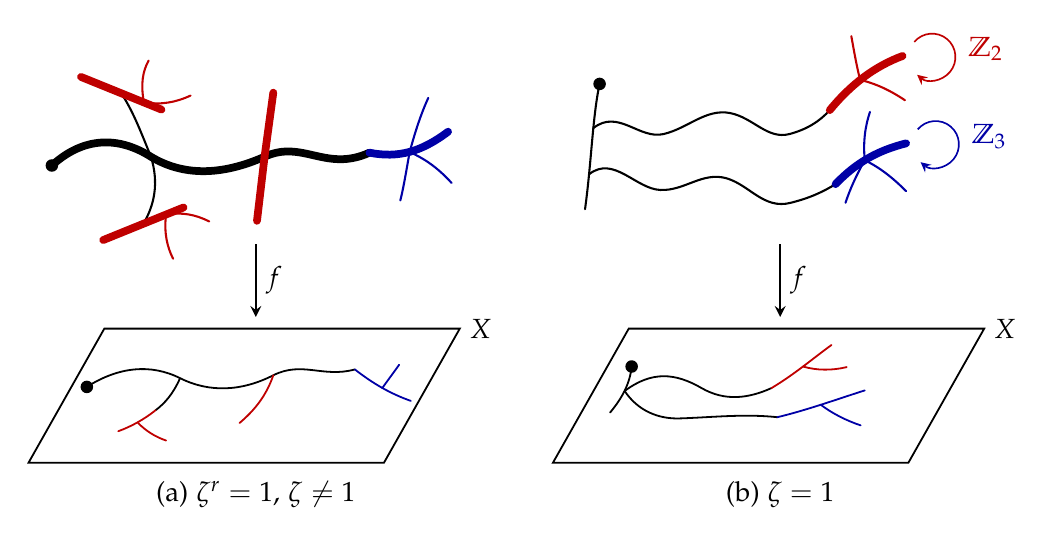
\begin{tikzpicture}[
        x=.74cm, y=.74cm,
        % Components of the domain curve. A cover style means the component
        % is a multiple cover of its image, drawn thick.
        dom/.style      ={black,         line width=.75pt, line cap=round},
        domcover/.style ={black,         line width=2.8pt, line cap=round},
        redcover/.style ={red!75!black,  line width=2.8pt, line cap=round},
        redtwig/.style  ={red!75!black,  line width=.75pt, line cap=round},
        bluecover/.style={blue!65!black, line width=2.8pt, line cap=round},
        bluetwig/.style ={blue!65!black, line width=.75pt, line cap=round},
        % Everything downstairs in X is drawn thin.
        img/.style      ={black,         line width=.65pt, line cap=round},
        redimg/.style   ={red!75!black,  line width=.65pt, line cap=round},
        blueimg/.style  ={blue!65!black, line width=.65pt, line cap=round},
        grparrow/.style ={->, >=stealth, line width=.6pt},
        fmap/.style     ={->, >=stealth, line width=.75pt},
        bull/.style     ={circle, fill=black, inner sep=1.6pt},
    ]

    %%%%%%%%%%%%%%%%%%%%%%%%%%%%%%%%%%%%%%%%%%%%%%%%%%%%%%%%%%%%%%%%%%%%%%%
    %% (a) zeta a primitive r-th root of unity, r >= 2.
    %%%%%%%%%%%%%%%%%%%%%%%%%%%%%%%%%%%%%%%%%%%%%%%%%%%%%%%%%%%%%%%%%%%%%%%
    \begin{scope}
        % The distinguished component: here g^r acts trivially on it, but g
        % does not, so it is a multiple cover of its image.
        \node[bull] at (-3.5,1.9) {};
        \draw[domcover]
            (-3.5,1.9)
            .. controls (-2.95,2.40) and (-2.35,2.40) .. (-1.80,2.05)
            .. controls (-1.25,1.72) and (-0.60,1.72) .. ( 0.15,2.05)
            .. controls ( 0.80,2.35) and ( 1.20,1.78) .. ( 1.95,2.12);

        % A leg meeting the distinguished component at a balanced node,
        % sticking out on both sides.  Each end carries a red multiple cover
        % together with the two branches interchanged by its automorphism.
        \draw[dom] (-1.80,2.05) .. controls (-2.00,2.55) and (-2.12,2.85) .. (-2.31,3.14);
        \draw[redcover] (-3.00,3.42) -- (-1.62,2.86);
        \draw[redtwig] (-1.92,2.98) .. controls (-1.98,3.30) and (-1.94,3.52) .. (-1.84,3.70);
        \draw[redtwig] (-1.92,2.98) .. controls (-1.62,2.94) and (-1.38,2.98) .. (-1.12,3.10);

        \draw[dom] (-1.80,2.05) .. controls (-1.66,1.60) and (-1.74,1.22) .. (-1.93,0.90);
        \draw[redcover] (-2.62,0.62) -- (-1.24,1.18);
        \draw[redtwig] (-1.54,1.06) .. controls (-1.58,0.74) and (-1.52,0.50) .. (-1.42,0.30);
        \draw[redtwig] (-1.54,1.06) .. controls (-1.26,1.10) and (-1.04,1.06) .. (-0.80,0.94);

        % A second balanced node, where the two legs are themselves the
        % multiple covers.
        \draw[redcover] (0.15,2.05) -- (0.30,3.15);
        \draw[redcover] (0.15,2.05) -- (0.02,0.95);

        % The tail: the part cut off at the unbalanced node.
        \draw[bluecover]
            (1.95,2.12) .. controls (2.45,2.02) and (2.85,2.14) .. (3.30,2.48);
        \draw[bluetwig] (2.64,2.13) .. controls (2.74,2.50) and (2.84,2.80) .. (2.96,3.06);
        \draw[bluetwig] (2.64,2.13) .. controls (2.58,1.80) and (2.54,1.54) .. (2.48,1.30);
        \draw[bluetwig] (2.64,2.13) .. controls (2.94,2.00) and (3.16,1.82) .. (3.36,1.60);

        \draw[fmap] (0,0.55) -- node[right] {$f$} (0,-0.70);

        % The target and the image of the map.
        \draw[img] (-3.9,-3.2) -- (2.2,-3.2) -- (3.5,-0.9) -- (-2.6,-0.9) -- cycle;
        \node[right] at (3.5,-0.9) {$X$};
        \node[bull] at (-2.90,-1.90) {};
        \draw[img] (-2.90,-1.90)
            .. controls (-2.35,-1.55) and (-1.80,-1.50) .. (-1.30,-1.75)
            .. controls (-0.80,-2.00) and (-0.25,-1.98) .. ( 0.30,-1.70)
            .. controls ( 0.80,-1.45) and ( 1.15,-1.75) .. ( 1.70,-1.60);
        % The two branches upstairs are folded onto the single one downstairs.
        \draw[img]    (-1.30,-1.75) .. controls (-1.42,-2.02) and (-1.56,-2.18) .. (-1.72,-2.30);
        \draw[redimg] (-1.72,-2.30) .. controls (-1.92,-2.46) and (-2.14,-2.58) .. (-2.36,-2.66);
        \draw[redimg] (-2.02,-2.52) .. controls (-1.88,-2.66) and (-1.72,-2.76) .. (-1.54,-2.82);
        \draw[redimg] ( 0.30,-1.70) .. controls ( 0.18,-2.05) and (-0.02,-2.30) .. (-0.28,-2.52);
        \draw[blueimg] (1.70,-1.60) .. controls (2.02,-1.85) and (2.32,-2.02) .. (2.66,-2.14);
        \draw[blueimg] (2.17,-1.92) .. controls (2.27,-1.78) and (2.36,-1.66) .. (2.46,-1.52);

        \node at (0,-3.75) {(a) \(\zeta^r = 1\), \(\zeta \neq 1\)};
    \end{scope}

    %%%%%%%%%%%%%%%%%%%%%%%%%%%%%%%%%%%%%%%%%%%%%%%%%%%%%%%%%%%%%%%%%%%%%%%
    %% (b) zeta = 1.
    %%%%%%%%%%%%%%%%%%%%%%%%%%%%%%%%%%%%%%%%%%%%%%%%%%%%%%%%%%%%%%%%%%%%%%%
    \begin{scope}[shift={(9,0)}]
        % Now g acts trivially on the distinguished component, so it is drawn
        % thin: it maps isomorphically onto its image.
        \node[bull] at (-3.10,3.30) {};
        \draw[dom] (-3.10,3.30) .. controls (-3.22,2.75) and (-3.24,1.95) .. (-3.35,1.15);
        \draw[dom] (-3.21,2.54)
            .. controls (-2.78,2.88) and (-2.42,2.34) .. (-2.00,2.44)
            .. controls (-1.58,2.54) and (-1.28,2.88) .. (-0.86,2.80)
            .. controls (-0.46,2.72) and (-0.22,2.34) .. ( 0.16,2.44)
            .. controls ( 0.46,2.52) and ( 0.68,2.66) .. ( 0.85,2.85);
        \draw[dom] (-3.28,1.75)
            .. controls (-2.86,2.08) and (-2.48,1.50) .. (-2.06,1.48)
            .. controls (-1.64,1.46) and (-1.34,1.80) .. (-0.92,1.68)
            .. controls (-0.52,1.56) and (-0.28,1.14) .. ( 0.18,1.26)
            .. controls ( 0.50,1.34) and ( 0.72,1.44) .. ( 0.95,1.58);

        % The arms: g acts nontrivially on them, through the indicated cyclic
        % group, which interchanges the thin branches sticking out.
        \draw[redcover] (0.85,2.85) .. controls (1.22,3.30) and (1.62,3.60) .. (2.10,3.78);
        \draw[redtwig] (1.37,3.37) .. controls (1.30,3.66) and (1.26,3.90) .. (1.22,4.12);
        \draw[redtwig] (1.37,3.37) .. controls (1.66,3.30) and (1.90,3.18) .. (2.14,3.02);
        \draw[grparrow, red!75!black]
            (2.30,4.02) arc[start angle=140, end angle=-130, radius=.40];
        \node[red!75!black, right] at (3.06,3.90) {$\Z_2$};

        \draw[bluecover] (0.95,1.58) .. controls (1.30,1.95) and (1.68,2.16) .. (2.16,2.28);
        \draw[bluetwig] (1.45,1.99) .. controls (1.42,2.32) and (1.46,2.58) .. (1.54,2.82);
        \draw[bluetwig] (1.45,1.99) .. controls (1.72,1.86) and (1.94,1.68) .. (2.16,1.46);
        \draw[bluetwig] (1.45,1.99) .. controls (1.30,1.72) and (1.20,1.50) .. (1.12,1.26);
        \draw[grparrow, blue!65!black]
            (2.36,2.52) arc[start angle=140, end angle=-130, radius=.40];
        \node[blue!65!black, right] at (3.12,2.40) {$\Z_3$};

        \draw[fmap] (0,0.55) -- node[right] {$f$} (0,-0.70);

        % The target and the image of the map.
        \draw[img] (-3.9,-3.2) -- (2.2,-3.2) -- (3.5,-0.9) -- (-2.6,-0.9) -- cycle;
        \node[right] at (3.5,-0.9) {$X$};
        \node[bull] at (-2.55,-1.55) {};
        \draw[img] (-2.55,-1.55) .. controls (-2.58,-1.85) and (-2.72,-2.10) .. (-2.92,-2.34);
        \draw[img] (-2.67,-1.97)
            .. controls (-2.20,-1.62) and (-1.80,-1.66) .. (-1.35,-1.92)
            .. controls (-0.95,-2.15) and (-0.55,-2.10) .. (-0.15,-1.92);
        \draw[img] (-2.67,-1.97)
            .. controls (-2.45,-2.30) and (-2.10,-2.46) .. (-1.70,-2.44)
            .. controls (-1.15,-2.42) and (-0.60,-2.36) .. (-0.05,-2.42);
        % Each arm is folded onto a single image curve with one branch.
        \draw[redimg] (-0.15,-1.92) .. controls (0.25,-1.68) and (0.55,-1.42) .. (0.88,-1.18);
        \draw[redimg] ( 0.39,-1.55) .. controls (0.63,-1.62) and (0.89,-1.62) .. (1.14,-1.56);
        \draw[blueimg] (-0.05,-2.42) .. controls (0.45,-2.30) and (0.95,-2.12) .. (1.45,-1.96);
        \draw[blueimg] ( 0.70,-2.21) .. controls (0.90,-2.36) and (1.14,-2.48) .. (1.38,-2.56);

        \node at (0,-3.75) {(b) \(\zeta = 1\)};
    \end{scope}
    \end{tikzpicture}
\caption{周祐正所述的\(I\bar{M}_{0,1}(X,\beta)\)的各个分量：}
    \label{fig:adelic-components}
\end{figure}

我们将解释 ~\Cref{fig:adelic-components}。设\(L_1\)为第一个标记点的切线丛，\(g\)为\(I\bar{M}_{0,1}(X,\beta)\)中某点的自同构。则\(\zeta\)由条件定义：\(g\)作用于\(L_1\)的特征值为\(\zeta\)。在两种图示中，箭头表示第一个标记点及其在\(X\)中的像，而粗线表示其为自身像的多覆盖的组成部分。

首先，假设\(\zeta = 1\)。此时，黑色部分是包含第一个标记点且\(g\)作用为恒等的极大连通分支。红色和蓝色部分是\(g\)作用非平凡的分支，我们称其为 \textit{ 枝 }。

现在假设\(\zeta\)是\(r\)阶的单位根（其中\(r \geq 2\)）。此时，黑色分支的节点在\(g\)作用下必须保持平衡，因此我们切去非平衡部分（着色为蓝色），并称其为 \textit{尾部}。在剩余部分中，黑色分支是包含第一个标记点且\(g^r\)作用为恒等态射的最大连通分支。最后，移除黑色分支和尾部后，我们将剩余的分支称为 \textit{支}。

% \begin{figure}[htpb]
%     \centering
%     \resizebox{\textwidth}{!}{%
%     \begin{tikzpicture}[
%         x=1cm,
%         y=1cm,
%         curve/.style={black, line width=1.25pt, line cap=round},
%         fixed component/.style={black, line width=3.2pt, line cap=round},
%         red component/.style={red!75!black, line width=3.2pt, line cap=round},
%         blue component/.style={blue!70!black, line width=3.2pt, line cap=round},
%         image curve/.style={black, line width=1.05pt, line cap=round},
%         action arrow/.style={->, >=stealth, line width=.75pt},
%         map arrow/.style={->, >=stealth, line width=.8pt},
%         marked point/.style={circle, fill=black, inner sep=1.8pt}
%     ]
%         % The case of a nontrivial r-th root of unity.
%         \begin{scope}[xshift=0cm]
%             \node[font=\large] at (0,5.95)
%                 {$r\geq 2,\qquad \zeta^r=1,\quad \zeta\neq 1$};
%
%             % Domain curve.
%             \node[marked point] (p1) at (-3.15,3.7) {};
%             \draw[fixed component]
%                 (p1) .. controls (-2.25,4.15) and (-1.55,4.2) ..
%                 (-1.15,3.92)
%                 .. controls (-0.55,3.45) and (0.35,3.45) ..
%                 (0.85,3.82)
%                 .. controls (1.35,3.35) and (1.85,3.45) ..
%                 (2.2,4.05);
%             \fill (-1.15,3.92) circle (2.2pt);
%             \fill (0.85,3.82) circle (2.2pt);
%             \fill (2.2,4.05) circle (2.2pt);
%
%             % Two legs attached to balanced nodes.
%             \draw[curve]
%                 (-1.15,3.92) .. controls (-1.25,4.45) and (-1.35,4.78) ..
%                 (-1.72,5.18);
%             \draw[red component]
%                 (-2.18,5.48) .. controls (-1.92,5.25) and (-1.65,5.08) ..
%                 (-1.36,5.02);
%             \draw[curve, red!75!black]
%                 (-1.67,5.14) .. controls (-1.64,5.35) and (-1.59,5.55) ..
%                 (-1.53,5.72);
%             \draw[curve, red!75!black]
%                 (-1.53,5.08) .. controls (-1.34,5.14) and (-1.18,5.25) ..
%                 (-1.02,5.4);
%             \draw[action arrow, red!75!black]
%                 (-1.9,5.38) arc[start angle=20,end angle=315,radius=.42];
%
%             \draw[curve]
%                 (-1.15,3.92) .. controls (-1.1,3.35) and (-1.25,3.0) ..
%                 (-1.62,2.63);
%             \draw[red component]
%                 (-2.18,2.32) .. controls (-1.9,2.56) and (-1.6,2.75) ..
%                 (-1.3,2.84);
%             \draw[curve, red!75!black]
%                 (-1.65,2.68) .. controls (-1.62,2.48) and (-1.59,2.25) ..
%                 (-1.54,2.06);
%             \draw[curve, red!75!black]
%                 (-1.5,2.76) .. controls (-1.31,2.7) and (-1.14,2.58) ..
%                 (-.98,2.42);
%             \draw[action arrow, red!75!black]
%                 (-1.85,2.57) arc[start angle=25,end angle=315,radius=.38];
%
%             % A second symmetric pair of balanced legs.
%             \draw[curve] (0.2,3.48) .. controls (0.16,4.05) and (0.2,4.35) ..
%                 (0.32,4.7);
%             \draw[red component] (0.2,3.9) -- (0.33,4.72);
%             \draw[curve] (0.2,3.48) .. controls (0.16,3.12) and (0.08,2.82) ..
%                 (-0.02,2.48);
%             \draw[red component] (0.11,3.05) -- (-0.03,2.46);
%
%             % The nonbalanced tail.
%             \draw[blue component]
%                 (2.2,4.05) .. controls (2.68,3.92) and (3.05,4.02) ..
%                 (3.48,4.3);
%             \draw[curve, blue!70!black] (2.86,4.08) -- (3.15,4.78);
%             \draw[curve, blue!70!black] (2.95,4.07) -- (2.88,3.35);
%             \draw[curve, blue!70!black] (2.95,4.07) -- (3.45,3.55);
%
%             % The target and the image of the map.
%             \draw[curve]
%                 (-3.55,-1.65) -- (2.48,-1.65) -- (3.48,1.0) --
%                 (-2.65,1.0) -- cycle;
%             \node[marked point] (xp1) at (-2.65,-0.25) {};
%             \draw[image curve]
%                 (xp1) .. controls (-2.05,0.04) and (-1.55,.22) ..
%                 (-1.15,.12)
%                 .. controls (-.5,-.05) and (-.2,-.1) ..
%                 (.12,.18)
%                 .. controls (.55,.55) and (1.0,.62) ..
%                 (1.55,.45);
%             % The first red orbit maps to a black connector followed by
%             % one red image curve; its two thin branches fold to the
%             % smaller red branch.
%             \draw[image curve]
%                 (-1.15,.12) .. controls (-1.23,-.08) and (-1.34,-.23) ..
%                 (-1.48,-.32);
%             \draw[red!75!black, line width=1.05pt, line cap=round]
%                 (-1.48,-.32) .. controls (-1.62,-.45) and (-1.78,-.58) ..
%                 (-1.92,-.65);
%             \draw[red!75!black, line width=1.05pt, line cap=round]
%                 (-1.69,-.51) .. controls (-1.58,-.64) and (-1.45,-.72) ..
%                 (-1.31,-.76);
%             \draw[red!75!black, line width=1.05pt, line cap=round]
%                 (.12,.18) .. controls (.02,-.22) and (-.25,-.38) ..
%                 (-.48,-.63);
%             \draw[blue!70!black, line width=1.05pt, line cap=round]
%                 (1.05,.57) .. controls (1.35,.12) and (1.68,-.18) ..
%                 (2.08,-.38);
%             \draw[blue!70!black, line width=1.05pt, line cap=round]
%                 (1.78,-.2) .. controls (1.82,-.08) and (1.88,.04) ..
%                 (1.96,.15);
%             \draw[map arrow] (0,2.62) -- node[right] {$f$} (0,1.22);
%             \node at (0,-2.1) {$(a)\ \zeta\neq 1$};
%         \end{scope}
%
%         % The untwisted eigenvalue case.
%         \begin{scope}[xshift=8.25cm]
%             \node[font=\large] at (0,5.95)
%                 {$I\overline{\mathcal M}_{0,1}(X,\beta),\qquad
%                   \on{Tr} g|_{L_1}=\zeta$};
%
%             % Domain curve: the thick portions have multiple covers onto
%             % their images.
%             \node[marked point] (p2) at (-2.95,4.45) {};
%             \draw[fixed component]
%                 (p2) .. controls (-3.08,3.85) and (-3.08,3.18) ..
%                 (-3.18,2.65);
%             \draw[curve]
%                 (-3.02,3.9) .. controls (-2.42,4.05) and (-2.0,3.62) ..
%                 (-1.62,3.72)
%                 .. controls (-1.18,3.3) and (-.72,3.18) ..
%                 (-.2,3.32);
%             \draw[curve]
%                 (-3.13,3.25) .. controls (-2.6,3.52) and (-2.25,2.88) ..
%                 (-1.8,2.68)
%                 .. controls (-1.25,2.4) and (-.68,2.42) ..
%                 (-.15,2.48);
%
%             % Nontrivial arms, shown in red and blue.
%             \draw[curve]
%                 (-.2,3.32) .. controls (.3,3.48) and (.5,3.72) ..
%                 (.76,3.92);
%             \draw[red component]
%                 (.76,3.92) .. controls (1.1,4.42) and (1.5,4.72) ..
%                 (2.02,4.9);
%             \draw[curve, red!75!black]
%                 (1.12,4.4) .. controls (1.08,4.68) and (1.05,4.92) ..
%                 (1.02,5.18);
%             \draw[curve, red!75!black]
%                 (1.55,4.7) .. controls (1.82,4.62) and (2.04,4.48) ..
%                 (2.25,4.3);
%             \draw[action arrow, red!75!black]
%                 (1.6,4.88) arc[start angle=210,end angle=-35,radius=.48];
%             \node[red!75!black, left] at (1.02,5.08) {$\Z_2$};
%
%             \draw[curve]
%                 (-.15,2.48) .. controls (.28,2.45) and (.55,2.64) ..
%                 (.86,2.76);
%             \draw[blue component]
%                 (.86,2.76) .. controls (1.18,3.13) and (1.52,3.32) ..
%                 (2.0,3.42);
%             \draw[curve, blue!70!black]
%                 (1.27,3.13) .. controls (1.34,3.4) and (1.43,3.65) ..
%                 (1.55,3.9);
%             \draw[curve, blue!70!black]
%                 (1.57,3.33) .. controls (1.83,3.2) and (2.05,3.02) ..
%                 (2.27,2.82);
%             \draw[action arrow, blue!70!black]
%                 (1.9,3.37) arc[start angle=145,end angle=-120,radius=.43];
%             \node[blue!70!black, above] at (2.55,3.62) {$\Z_3$};
%
%             % Target X and the images of the colored components.
%             \draw[curve]
%                 (-3.55,-1.65) -- (2.48,-1.65) -- (3.48,1.0) --
%                 (-2.65,1.0) -- cycle;
%             \node[marked point] (xp2) at (-2.05,.02) {};
%             \draw[image curve]
%                 (xp2) .. controls (-2.0,-.32) and (-2.35,-.62) ..
%                 (-2.62,-.93);
%             \draw[image curve]
%                 (-2.25,-.52) .. controls (-1.82,-.12) and (-1.55,-.12) ..
%                 (-1.14,-.42)
%                 .. controls (-.88,-.62) and (-.54,-.63) ..
%                 (-.22,-.52);
%             \draw[image curve]
%                 (-2.25,-.52) .. controls (-2.58,-.44) and (-2.75,-.62) ..
%                 (-2.98,-.83);
%             \draw[red!75!black, line width=1.05pt]
%                 (-.22,-.52) .. controls (.22,-.13) and (.5,.22) ..
%                 (.82,.48);
%             % The two thin red branches upstairs fold to this one
%             % additional branch of the red image curve.
%             \draw[red!75!black, line width=1.05pt, line cap=round]
%                 (.345,.029) .. controls (.57,-.02) and (.77,.06) ..
%                 (1.0,.18);
%             % A chain of black components joins the blue image to the
%             % distinguished black component.
%             \draw[image curve]
%                 (-2.25,-.52) .. controls (-2.12,-.76) and (-2.0,-.91) ..
%                 (-1.88,-1.0);
%             \draw[image curve]
%                 (-1.88,-1.0) .. controls (-1.76,-.82) and (-1.53,-.91) ..
%                 (-1.38,-1.18);
%             \draw[image curve]
%                 (-1.38,-1.18) .. controls (-.65,-.76) and (.08,-.68) ..
%                 (.78,-.72);
%             \draw[blue!70!black, line width=1.05pt, line cap=round]
%                 (.78,-.72) .. controls (1.24,-.74) and (1.58,-.62) ..
%                 (1.98,-.32);
%             \draw[map arrow] (0,2.03) -- node[right] {$f$} (0,1.22);
%             \node at (0,-2.1) {$(b)\ \zeta=1$};
%         \end{scope}
%     \end{tikzpicture}%
%}
%     \caption{一个分量的分解：
%     \(I\overline{\mathcal M}_{0,1}(X,\beta)\) into its distinguished
%     周祐正提供的分量、腿（或臂）与尾；粗线表示多重覆盖其像的分量。
%     that map with degree greater than one onto their images. Symmetric
%     branches occur on the domain, and \(f\) folds each orbit to a single
%     image curve in \(X\).}
%     \label{fig:adelic-components}
% \end{figure}
%
% We will now explain the meaning of the different parts of~\Cref{fig:adelic-components}. Let \(L_1\)
% be the cotangent line at the first marked point and define \(\zeta\) by
% \[
%     g|_{L_1}=\zeta\,\mr{Id}_{L_1}.
% \]
% The bullets denote the first marked point and its image in \(X\), and a
% thick curve denotes a component that is a multiple cover of its image.
% The black component is the maximal connected component containing the
% first marked point on which \(g\) acts trivially when \(\zeta=1\). The red
% and blue components on which \(g\) acts nontrivially are called
% \textit{arms}.
%
% More generally, suppose that \(\zeta\) is an \(r\)-th root of unity with
% \(r\geq 2\). The nodes of the thick black component must be balanced with
% respect to the \(g\)-action. Cut off the part attached at an unbalanced
% node (the blue component in the figure); this part is called the
% \textit{尾部}. In what remains, the thick black component is the maximal
% connected component containing the first marked point on which \(g^r\)
% acts trivially. After removing the black component and the tail, the
% remaining components are called \textit{支}.

Givental 定义如下：
\[ \ab<\frac{\Phi}{1-qL}>_{0,1,\beta}^{X,K} \coloneqq \sum_{\zeta} \ab<\frac{\Phi}{1-qL}>_{0,1,\beta}^{X_{\zeta}}, \]
其中\(X_{\zeta}\)项仅由 Riemann-Roch 定理下的\(M_{\zeta}\)贡献。现在，我们定义枝、腿和尾。此处，定义 \textit{ 枝}
\[ \mr{arm}(q) \coloneqq \sum_{\beta, \alpha, \zeta \neq 1} Q^{\beta} \Phi^{\alpha}\ab<\frac{\Phi_{\alpha}}{1-qL}>_{0,1,\beta}^{X_{\zeta}}, \]
\textit{ 腿}
\[ \mr{leg}_{\zeta}(q) \coloneqq \mr{leg}_r(q) = \Psi^r (\mr{arm}(q)), \]
和 \textit{ 尾}
\[ \mr{tail}_{\zeta}(q) \coloneqq \sum_{\beta, \alpha, \zeta' \neq \zeta} Q^{\beta} \Phi^{\alpha} \ab<\frac{\Phi_{\alpha}}{1-qL}>_{0,1,\beta}^{X_{\zeta'}}. \]

\begin{prop}[{\cite{GiventalTonita2014}}]
\(J\)-函数在\(q = 1\)处的 Laurent 展开式为
    \begin{align*}
        J^K(0)_{q=1} &= J^{\mr{fake}}(\mr{arm}(q)) \\
        &\coloneqq 1-q + \mr{arm}(q) + \sum_{n,\beta,\alpha} \frac{Q^{\beta}\Phi^{\alpha}}{n!} \ab<\frac{\Phi_{\alpha}}{1-qL}, \mr{arm}(L), \ldots, \mr{arm}(L)>_{0,n+1,\beta}^{\mr{fake}},
    \end{align*}
其中，假不变量通过应用 Riemann-Roch 定理并仅考虑未扭曲子空间的贡献计算得出。
\end{prop}

\begin{prop}[{\cite{GiventalTonita2014}}]
在任何其他单位根\(\zeta \neq 1\)的情形下，我们有
    \begin{align*}
        &J^K(0)_{q = \zeta} = (1-q) + \mr{tail}_{\zeta}(q) \\
        &+ \sum_{n,\beta,\alpha} \frac{Q^{r\beta}\Phi^{\alpha}}{n!} \ab[\frac{\Phi_{\alpha}}{1-\zeta q L^{1/r}}, \mr{leg}_r(L), \ldots, \mr{leg}_r(L), 1 - \zeta^{-1}L^{1/r} + \mr{tail}_{\zeta}(\zeta^{-1} L^{1/r})]^{\mr{stem}},
    \end{align*}
其中茎是定义在模空间上的某个伪不变量\(X \times B\mu_r\)
    \[ \bar{M}_{0,n+2,\beta}^X(\zeta) \coloneqq \bar{M}_{0,n+2}(X \times B\mu_r, \beta, (g, 1, \ldots, 1, g^{-1})). \]
由下式定义
    \begin{align*}
        [\cdots]^{\mr{stem}} \coloneqq \int_{[\bar{M}_{0,n+2,\beta}^X(\zeta)]^{\vir}} \on{td}(T_{\bar{M}}) \on{ch}\ab(\frac{\on{Tr}(\cdots)}{\on{Tr}(\lambda_{-1}(N^*))}), 
    \end{align*}
其中\(N\)表示\(\bar{M}_{0,n+2,\beta}^X(\zeta) \subset \bar{M}_{0,nr+2}(X, r\beta)\)的法向量丛。
\end{prop}

\begin{rmk}
若我们能够计算伪理论与茎理论，则可计算亏格零量子 K 不变量。
\end{rmk}

\subsection{量子\(K\)-理论的一个点}%
\label{sub:Quantum K-theory of a point}

一个自然的问题是研究高亏格量子\(K\)-理论。我们先从最简单的靶空间——一个点——开始。研究高亏格理论的动机之一，是尝试证明 Klemm--Pandharipande 为 Calabi--Yau 四维簇定义的 GV 不变量，或 Pandharipande--Zinger 为 Calabi--Yau 五维簇定义的 GV 不变量具有整性；后一种情形只需考虑亏格\(1\)。之所以先研究点的量子\(K\)-理论，是因为\(I\bar{M}_{1,1}(X, \beta)\)有一些分量会把整条亏格\(1\)曲线收缩到一点。

\begin{quest}
K-理论 Witten-Kontsevich 定理是什么？\footnote{ 根据周祐正，困难之处在于处处存在。}
\end{quest}

我们首先回顾上同调 Witten 猜想。我们从算子开始
\[ L = \partial_x^2 + u(x) \]
并将其变形为
\[ \tilde{L} = \partial_x^2 + u(x, T_3, T_5, \ldots), \]
其中我们应将\(x = T_1\)和\(u(x) = u(x, 0, 0,\ldots)\)视为。形式上，写为
\[ L^{1/2} = \partial_x + \sum_{k > 0} a_{-k}(x) \partial_x^{-k} \]
利用性质
\[ \partial^n \circ f = \sum_{m = 0}^{\infty} \binom{n}{m} f^{(m)} \partial^{n-m} \]
对所有整数\(n \in \Z\)成立。特别地，我们通过方程构造 (2-)KdV 族
\[ \pdv{\tilde{L}}{T_{2k+1}} = \ab[(\tilde{L}^{\frac{2k+1}{2}})_{\geq 0}, \tilde{L}] \]
对所有\(k \geq 0\)成立。我们称函数\(\tau\)为\textit{\(\tau\)-函数}，如果
\[ 2 \pdv[2]{}{x}\log \tau(x, T_3, T_5, \ldots) = u(x, T_3, T_5, \ldots). \]
现在使用\(u = 2x\)执行上述过程。定义函数
\[ F(t_0, t_1, \ldots) \coloneqq \sum_{n \geq 0} \sum_{k_0, \ldots, k_n} \ab<\tau_0^{k_0} \cdots \tau_n^{k_n}> \frac{t_0^{k_0} \cdots t_n^{k_n}}{k_0! \cdots k_n!}. \]
注意，由于亏格完全由插入项的数量和插入项的度决定，记号
\[ \ab<\tau_0^{k_0} \cdots \tau_n^{k_n}> \]
唯一确定了一个点的后裔 GW 不变量。

\begin{thm}[Kontsevich {\cite{Kontsevich1992}}]
\(F\)是在变量替换\(t_i = (2i+1)!! T_{2i+1}\)下，以\(L = \partial_x^2 + 2x\)为起点构造的 KdV 族的\(\tau\)函数。
\end{thm}

该定理的一个应用是考虑虚拟局部化。例如，假设我们考虑\(\bar{M}_{g,0}(X, d[C])\)，其中\(C\)是一个 Calabi-Yau 三重曲面 Calabi--Yau 三维簇中的唯一有理曲线，其法向量丛为\(N = \mc{O}(-1)\oplus \mc{O}(-1)\)。在此设定下，我们可简化为局部模型并计算
\begin{align*}
    \int_{[\bar{M}_{g,0}(\P^1, d)]^{\vir}} c_{\mr{top}}(R^1 \pi_* N) = \sum_{m \vdash d} \frac{(-1)^{d-L(m)}}{\abs{\Aut(m)}} \int_{\bar{M}_{g, L(m)}} \frac{1 + \cdots + c_g(\mc{H})}{\prod_i (1-m_i \psi_i)}
\end{align*}
通过虚拟局部化。若我们希望在\(K\)-理论中获得类似结果，则需考虑形式
\[ \chi\ab(\bar{M}_{g, L(m)}/\Aut(m), \frac{\lambda_{-1}(\mc{H})}{1-m_i L_i}), \]
因此，我们需要考虑一个点的置换等变量子\(K\)-理论。

我们现在进行文献综述。首先，李元斌~\cite{Lee1997} 计算了公式
\[ \ab<\frac{1}{1-q_1 L}, \ldots, \frac{1}{1-q_n L}>_{0,n}^{\mr{pt}, K} = \ab(\prod_{i=1}^n \frac{1}{1-q_i}) \ab(1 + \sum_{i=1}^n \frac{q_i}{1-q_i})^{n-3}. \]
随后，李元斌与瞿枫~\cite{LeeQu2014} 提供了一种计算方法
\[ \ab<\frac{1}{1-q_1 L}, \ldots, \frac{1}{1-q_n L}>_{1,n}^{\mr{pt}, K} \]
在原则上。Givental~\cite{Givental2017K1} 计算了公式
\[ \sum_{n \geq 2} \ab<\frac{1}{1-q L}, 1, \ldots, 1>_{0,1+n}^{S_n} = (1-q) \exp\ab(\sum_{k > 0} \frac{\Psi^k}{k} \ab(1 + \frac{q}{1-q})). \]
最后，Milanov~\cite{Milanov2025} 在 2024 年首次发布的预印本中计算了
\begin{align*}
    \sum_{n \geq 0}& \ab<\frac{1}{1-q_1 L}, \ldots, \frac{1}{1-q_r L}, 1, \ldots, 1>_{0,r+n}^{S_n} \\
    &= \ab(\prod_{i=1}^{r} \frac{1}{1-q_i})\ab(1 + \sum_{i=1}^r \frac{q_i}{1-q_i}) \exp\ab(\sum_{k > 0} \frac{\Psi^k}{k} \ab(1 + \sum_{i=1}^r \frac{q_i}{1-q_i})). 
\end{align*}

下面的多重 Hodge 递推及由此得到的新的亏格一计算由周祐正给出，并在本次讲座中报告。

设\(s \in \Z\)，并定义其多重霍奇层为\(\mc{H}_s \coloneqq R^0 \pi_* (\omega_{\pi}^s)\)。考虑态射\(\bar{M}_{g,n+1} \xrightarrow{\pi} \bar{M}_{g,n}\)，我们将上层余切线记为\(L_i\)，下层余切线记为\(\ell_i\)。

\begin{lem}
对于所有整数\(s\)和\(d_i\)，我们有
    \[ \pi_*\ab(\omega_{\pi}^s\ab(\sum_{i=1}^n d_i D_i)) = \mc{H}_s-\mc{H}_{1-s}^* + \sum_{i=1}^n \sum_{k=1}^{d_i} \ell_i^{-k+s}. \]
\end{lem}

\begin{rmk}
    注意，若\(f(q) \in \Z[q]\)，则\(\exp \sum_k \frac{\Psi^k}{k} (f(q)) \in \Z \ps{q}\)。这是因为该操作将\(f = \sum_{i=1}^{n} a_i q^i\)映射到\(\prod_{i=1}^n \frac{1}{(1-q^i)^{a_i}}\)。
\end{rmk}

\begin{proof}
    当所有\(d_i\)为零时，我们发现
    \[ R^0 \pi_* \omega_{\pi}^s - R^1 \pi_* \omega_{\pi}^s = \mc{H}_s - \mc{H}_{1-s}^* \]
由 Serre 对偶性可知。下一步需证明
    \[ \pi_* \omega_{\pi}^s ((r+1)D_i) = \pi_* \omega_{\pi}^s(r D_i) + \ell_i^{s-r-1}. \]
此处，我们首先考虑正合列
    \[ 0 \to \mc{O} (-D_i) \to \mc{O} \to \mc{O}_{D_i} \to 0 \]
    并通过\(\omega_{\pi}^s\)扭转，以获得
    \[ 0 \to \omega_{\pi}^s(r D_i) \to \omega_{\pi}^s ((r+1)D_i) \to \omega_{\pi}^s ((r+1)D_i) \otimes \mc{O}_{D_i} \to 0 \]
    然后计算前推。
\end{proof}

\begin{lem}
    设\(f_i\)为有理函数，例如\(\frac{1}{1-q L}\)。此时
    \begin{align*}
        \ab<f_1(L), \ldots, f_n(L), L_{n+1}^r>_{g, n+1} ={}& \sum_{i=1}^n \ab<f_1(L), \ldots, D(f_i f_{n+1}), \ldots, f_n(L)>_{g, n} \\
        &+ \ab<f_1(L), \ldots, f_n(L) \mid \mc{H}_r - \mc{H}_{1-r}^*>_{g,n},
    \end{align*}
    其中\(f_{n+1} = L_{n+1}^r\)和\((Df)(x) \coloneqq \frac{f(x)-f(1)}{x-1}\)。
\end{lem}

要证明这一点，我们需要考虑前推。
\begin{align*}
    \pi_* (L_1^{d_1} \cdots L_{n+1}^{d_{n+1}}) &= \pi_* \ab(\pi^*(\ell_1^{d_1} \otimes \cdots \otimes \ell_n^{d_n}) \otimes \omega_{\pi}^{d_{n+1}}\ab(\sum_i (d_i+d_{n+1})D_i)).
\end{align*}
在此，我们利用\(L_i = (\pi^* \ell_i)(D_i)\)和\(L_{n+1} = \omega_{\pi}(D_1 + \cdots + D_n)\)这一事实。根据前面的引理，可以看出前推变为
\[ (\ell_1^{d_1} \cdots \ell_n^{d_n})\ab(\mc{H}_{d_{n+1}} - \mc{H}_{1-d_{n+1}}^* + \sum_{i=1}^n \sum_{k=1}^{d_i + d_{n+1}} \ell_i^{-k+d_{n+1}}). \]
现在，李元斌的公式计算关联子。
\[ \ab<(L-1)^{k_1}, \ldots, (L-1)^{k_n}>_{0,n} = \frac{(n-3)!}{\prod_{i=1}^n k_i! \ab(n-3-\sum_i k_i)!} \]
通过展开
\[ \frac{1}{1-qL} = \frac{1}{1-q} \sum_{k \geq 0} \frac{q^k(L-1)^k}{(1-q)^k}. \]
注意这里亏格\(0\)中没有 Hodge 丛，因此实际上可以利用该引理得到李元斌的公式。

\begin{lem}
我们有
    \[ \mc{H}_r - \mc{H}_{1-r}^* = \pi^* (\mc{H}_r - \mc{H}_{1-r}^*) - \sum_{i=1}^n (D^2 (\pi^* \ell_i)^r) \mc{O}_{D_i}. \]
\end{lem}

这些引理共同表明，我们可以将问题简化为单一标记的情况，代价是插入变得极为复杂，并到处引入多重霍奇项。在亏格中，情况变得简单，因为在\(1\)上，我们有\(\bar{M}_{1,1}\)。
\[ \mc{H}_r = \mc{O}(r) = L_1^r. \]
此时，回忆经典公式
\[ \chi\ab(\bar{M}_{1,1}, \frac{1}{1-qL}) = \frac{1}{(1-q^4)(1-q^6)}. \]
不幸的是，计算
\[ \chi\ab(\bar{M}_{1,n}; \frac{1}{1-q_1 L} \cdots \frac{1}{1-q_n L}) \]
过于困难，因此尝试计算
\[ \chi\ab(\bar{M}_{1,1}; \frac{1}{1-q_1 L_1} \cdots \frac{1}{1-q_n L_1})  \]
该表达式已知，但尚不清楚如何写出其良好形式的公式。考虑该操作的原因在于
\[ \Z\ps{q} \xrightarrow{[]_r} \Z\ps{q_1, \ldots, q_r} \qquad q^k \to h_k(q_1, \ldots, q_r) \coloneqq \sum_{\ell_1 + \cdots + \ell_r = k} q_1^{\ell_1} \cdots q_r^{\ell_r}. \]
遗憾的是，周祐正未能把它写成较为简洁的形式：
\[ \chi\ab(\bar{M}_{1,1}; \frac{1}{1-q_1 L_1} \cdots \frac{1}{1-q_n L_1}) = \ab[\frac{1}{(1-q^4)(1-q^6)}]_n \]
在原则上，我们可写出类似
\[ [f(q)]_2 \coloneqq \frac{q_1 f(q_1) - q_2 f(q_2)}{q_1 - q_2}, \]
的公式，但此方法似乎帮助不大。

\subsection{点的置换等变理论}%
\label{sub:Permutation-equivariant theory of a point}

我们可以通过另一种方式计算\(\chi\ab(\bar{M}_{1,1}, \frac{1}{1-q L})\)。考虑椭圆曲线上的一个对合，它给出了一个映射
\[ \bar{M}_{1,1} \to \bar{M}_{0,1+3}/S_3. \]
则 Givental~\cite{Givental2017K1} 计算
\[ \chi\ab([\bar{M}_{0,1+n-1}/S_{n-1}], \frac{1}{1-qL}) = \prod_{i=2}^{n-1} \frac{1}{1-q^i}. \]
特别地，我们得到
\[ \frac{1}{(1-q^2)(1-q^3)}, \]
然后由于该映射是一个\(\mu_2\)-层（或对象上的\(2:1\)-覆叠），我们即可得到所需的公式。

考虑\(\mc{H}_{g,1} \subset \bar{M}_{g,1}\)为超椭圆轨迹。注意标记位于一个 Weierstrass 点。注意超椭圆对合的不动点映射到\(2g+1\)个\(\P^1\)上的点，因此我们希望利用该计算
\[ \chi\ab(\bar{M}_{0,1+2g+1}/S_{2g+1}, \frac{1}{1-q L}) = \prod_{i=2}^{2g+1} \frac{1}{1-q^i} \]
来求解该量
\(\chi\ab(\mc{H}_{g,1}, \frac{1}{1-qL})\)。然而，由于上层曲线退化的性质，我们需要考虑哈塞特（Hassett）模空间~\cite{Hassett2003}，其中最后\(2g+1\)个标记的权重为\(\frac{1}{2}\)。
 






\section{拟映射穿墙（周杨）}%
\label{sec:Quasimap wall-crossing (周杨)}

本讲座的主要穿墙定理与主空间构造见~\cite{Zhou2022}。较早的亏格零与高亏格结果见~\cite{CFK2014,CFK2020}；稳定拟映射的基础理论见~\cite{CFKM2014}。

令\(X\)表示五次三维簇。我们的目标是计算亏格零曲线在\(X\)上的数量，该问题由 Givental 和 Lian-Liu-Yau 解决。通过闭浸入\(X \subset \P^4\)，我们可以表示
\[ \bar{M}_0(X, d) \subset \bar{M}_0(\P^4, d), \]
该对象为光滑，且具有由\((\C^{\times})^5\)引起的环面作用。若映射被此作用固定，则其定义域必须包含一些映射至不动点的分量，以及一些构成\(n :1\)重覆盖\(1\)维轨道的分量。特别地，不动点轨迹由一组图结构索引。

在此设定下，我们有量子勒夫舍茨原理，其表述为
\[ [\bar{M}_0(X, d)]^{\on{vir}} = e(E) \cap [\bar{M}_0(\P^4, d)]. \]
此处，向量丛\(E\)由
\[ E = \pi_* f^* \mc{O}(5), \]
其中\(\pi\)为 universal curve，\(f\)为 universal 稳定映射。我们将从不同角度重新阐释该结果：若
\begin{align*}
    I(q, z) &= 1 + \sum_{d > 0} \frac{\prod_{k=1}^{5d} (5H+kz)}{\prod_{k=1}^d (H+kz)^5} q^d \in H^*(X)[z^{-1}] \ps{q} \\
    &= I_0(q) \cdot 1 + I_1(q) \frac{H}{z} + I_2(q) \frac{H^2}{z^2} + I_3(q) \frac{H^3}{z^3},
\end{align*}
则
\[ J (Q, z) = 1+ \sum_{d>0} \phi^{\alpha} \ab<\frac{\phi_{\alpha}}{z(z-\psi)}>_{0,1}^X Q^d = \frac{I}{I_0} \]
在镜像映射\(Q = q \exp\ab(\frac{I_1}{I_0})\)的作用下。

\subsection{天真的计数}%
\label{sub:Naive counting}

考虑从固定的\(\P^1\)到\(X \subset \P^4\)的映射。为简化记号，假设\(X = \ab(\sum x_i^5 = 0)\)是 Fermat 五次三维簇。这样的映射由一组\([f_0, \ldots, f_4]\)给出，其中\(f_i \in \C[u,v]\)、\(\deg f_i = d\)，并满足\(\sum f_i^5 = 0\)。若要得到真正的态射，还须要求各\(f_i\)没有公共零点；但所得模空间并不固有，所以我们放宽这一条件，改为考虑下面的模空间。
\[ QG(X, d) =  \ab\{ [f_0, \ldots, f_4] \middle\vert \Vectorstack{{ f_i \in \C[u,v] } { \deg f_i = d }}, \sum f_i^5 = 0, (f_0, \ldots, f_4) \neq (0,\ldots, 0) \} \bigg/ \C^{\times}. \]
该结构嵌入在对应的模空间中
\begin{align*}
    QG(\P^4, d) &\coloneqq  \ab\{ [f_0, \ldots, f_4] \mid f_i \in \C[u,v], \deg f_i = d, (f_0, \ldots, f_4) \neq (0, \ldots, 0) \} \\
    &\cong \P^{5d+5-1} 
\end{align*}
的有理映射到射影空间。存在两个问题：首先，定义域参数化，需考虑\(\P^1\)的自同构；其次，为获得稳定映射，需对定义域进行吹胀。

首先，令\(\C^{\times}\)通过缩放\(u\)作用于\(\P^1\)。考虑由\(F_{\star} \subset QG(X, d)\)定义的特殊不动点轨迹，其满足
\[ F_{\star,d} = \ab\{ [f_0, \ldots, f_4] \text{ 为不动点，且 } (v=0) \text{ 不是公共零点} \}. \]
因此，\(F_{\star,d} = \ab\{ [a_0 u^d, \ldots, a_4 u^d] \mid [a_0, \ldots, a_4] \in X \} \cong X\)。从该视角，可将\(I\)-函数重写为
\begin{align*}
    I(q,z) &= \sum_{d > 0} \ab(\frac{[F_{\star, d}]^{\vir}}{e_{\C^{\times}}(N^{\vir})})^{\mr{PD}} q^d \\
    &= 1 + \sum_{d > 0} \ab( \frac{[X]}{e_{\C^{\times}}(N^{\vir})})^{\mr{PD}} q^d
\end{align*}
利用变形理论中的标准方法。该结构嵌入在\(H^*_{\C^{\times}}(X) \ps{q}[z^{-1}]\)中。

\subsection{穿墙无严格性}%
\label{sub:Wall-crossing without rigor}


其次，考虑带标记和尾部的节点曲线\(C\)，其尾部具有\(\C^{\times}\)作用。假设存在映射\(f \colon C \to X\)。若取极限
\[ \lim_{t \to 0} [f_0(t^{-1}u, v), \ldots, f_4(t^{-1}u, v)] = [a_0 u^{d_0}, \ldots, a_4 u^{d_0}], \]
则极限气泡将落入\(F_{\star, d_0}\)，其中公共零点远离节点。随后，可将该尾部替换为新标记，其携带\(I\)-函数的部分项。对于五次三维簇，其形式为\(I_1 H - I_0 \psi = [zI-z]_{+, z = -\psi}\)。最终，我们得到\(C = \P^1\)，其包含\(I\)-函数的多种贡献。

注意，若考虑\(\C^{\times}\)作用于\(\P^4\)，则\(f \colon C \to \P^4\)固定时需满足：对所有\(t \in \C^{\times}\)，存在\(\varphi_t\)使得
\begin{equation*}
\begin{tikzcd}
    C \ar{r}{f} \ar{d}[swap]{\varphi_t} & \P^4 \\
    C \ar{ur}[swap]{t \cdot f}
\end{tikzcd}
\end{equation*}
该图则可交换。因此，我们得到\(\C^{\times}\)在定义域上的作用。

我们定义到\(X\)的\(\ep\)-稳定拟映射模空间\(Q_{g,n}^{\ep}(X, d)\)，它与稳定映射模空间类似。可以把不同\(\ep\)对应的模空间看作虚拟双有理等价；每个空间都是带完美障碍理论的固有 DM 叠，因此可定义拟映射不变量
\[ \ab< \gamma_1 \psi_1^{a_1} \cdots \gamma_n \psi_n^{a_n}>_{g,n}^{\ep} \coloneqq \int_{[Q_{g,n}^{\ep}(X,d)]^{\vir}} \prod_{i=1}^n \ev_i^*(\gamma_i) \psi_i^{a_i}. \]
这里\(\ep \in \Q_{>0}\)为正有理数。\(\ep\)的参数空间具有墙室结构，墙位于\(\frac{1}{n}\)，其中\(n\)为正整数。当\(\ep > 1\)时得到Gromov--Witten 理论（即稳定映射）；向左穿墙时，允许的有理尾更少，但允许更多基点。最终在\(\ep \to 0^+\)极限下不再允许有理尾。于是，在墙\(\frac{1}{d_0}\)附近得到如下穿墙公式：
\[ \ab<->_{g,n,d}^{\ep_+} - \ab<->_{g,n,d}^{\ep_-} = \sum_{k} \frac{1}{k!} \ab<-, \mu, \ldots, \mu>_{g,n+k, d-kd_0}^{\ep_+}. \]
此处，\(\mu = [zI-z]_{+, q^{d_0}, z=-\psi}\)。在特例中，若\(g = 0\)，\(n = 1\)，且\(\ep = 0^+\)，则有
\[ \sum \phi^{\alpha} \ab<\frac{\phi_{\alpha}}{z(z-\psi)}>^{\ep}_{0,1} = I_{z^{<0}}. \]
穿越所有 GW 室的墙后，我们得到
\[ I = 1 + \sum_{\substack{d \geq 1 \\ k \geq 0}} \frac{1}{k!} \sum_{\alpha} \phi^{\alpha} \ab< \frac{\phi_{\alpha}}{z(z-\psi)}, I_1 H - I_0 \psi, \ldots, I_1 H - I_0 \psi>_{0,1+k,d}^{\infty} q^d, \]
这通过微分和除子方程产生镜像映射

\subsection{拟映射}%
\label{sub:Quasimaps}

\begin{defn}
    到五次三维簇\(X\)的一个\textit{预稳定拟映射}由以下数据组成：
    \[(C, x_1, \ldots, x_n, \mc{L}, \varphi_0, \ldots, \varphi_4),\] 
    其中\((C, x_1, \ldots, x_n)\)是一个预稳定曲线，\(\mc{L} \in \Pic C\)，且\(\varphi_0, \ldots, \varphi_4 \in H^0(C, \mc{L})\)，使得
    \[ \varphi^{-1}(0) \coloneqq \ab\{x \in C \mid \varphi_0(x) = \cdots = \varphi_4(x) = 0 \} \]
    该空间是有限的且远离特殊点。此外，我们要求\(\sum \varphi_i^5 = 0\)。
\end{defn}

重要地，我们将\(\varphi^{-1}(0)\)称为 \textit{基点}。在\(\varphi^{-1}(0)\)之外，我们确实有一个态射\(C \setminus \varphi^{-1}(0) \to X\)。几何上，假设我们有一个\(\A^1 \setminus 0\)上的族，当\(t \to 0\)时，零轨迹\(\varphi_i^{-1}(0)\)会发生碰撞。我们可以选择在中心纤维中保留这个拟映射，或者通过多次吹扩中心纤维来获得一个实际的态射，代价是吹出一个有理尾。因此，任何模空间的准稳定拟映射都无法分离，我们必须考虑某种稳定性条件。

\begin{defn}
    预稳定拟映射\((C, \mathbf{x}, \mc{L}, \varphi)\)称为\textit{\(\ep\)-稳定}，如果
    \begin{enumerate}
        \item 对所有\(x \in \varphi^{-1}(0)\)，有\(\on{len}(x) \leq \frac{1}{\ep}\)，其中\(\on{len}(x) = \min \ab\{ \on{ord}_x (\varphi_i)\}\)；
        \item \(\Q\)-线丛\(\mc{L}^{\ep} \otimes \omega_C^{\log}\)在\(C\)的每个不可约分量上具有正的度。
    \end{enumerate}
\end{defn}

对每个不可约分量\(C' \subseteq C\)，都有\(\deg \mc{L}|_{C'} \geq 0\)。因此，稳定性会随\(\ep\)变化的，只可能是带至多两个特殊点的亏格零分量，或没有标记点的亏格一分量。在\((0,0)\)和\((1,0)\)两种情形中有\(C=C'\)；在\((0,2)\)情形中，稳定性等价于\(\deg\mc{L}>0\)；而在\((0,1)\)情形中，第二个条件等价于
\[ \deg \mc{L}|_{C'} > \frac{1}{\ep}. \]

\begin{exm}
    在\(\ep > 1\)室中，注意第一个条件意味着没有基点，第二个条件意味着所有不稳定分量具有正的度，因此我们恢复了稳定映射。

    若转移至\(\frac{1}{2} < \ep < 1\)室，则必须收缩度为\(1\)的有理尾部。例如，若有一条由两个度为\(1\)的有理曲线组成的链，且以尾部结束，则收缩最外层的尾部，剩下一个度为\(2\)的有理尾部，且带有一个长度为\(1\)的基点。

若我们进入\(\frac{1}{3} < \ep < \frac{1}{2}\)所在的腔室，则必须收缩所有度\(2\)的有理尾，并用长度为\(2\)的基点替换。
\end{exm}

\begin{rmk}
在射影空间的情形下，存在一个实际的态射
    \[ Q_g^{\ep_+}(\P^N, d) \to Q_g^{\ep_-}(\P^N, d) \qquad (C_g \cup C_0, \mc{L}, \varphi) \mapsto (C_g, \mc{L}|_{C_g}(p), \varphi(p)). \]
对于一般的目标空间，这并非可能，但该思想为拟映射穿墙现象提供了直观。
\end{rmk}

我们现在将讨论如何将此推广至更一般的目标空间。令
\[ X = V \sslash_{\theta} G, \]
其中\(V\)为仿射空间，\(G\)为可约双群，且\(\theta\)为\(G\)的一个特征。我们需要要求
\begin{enumerate}
    \item \(V^{\mr{ss}}(\theta) = V^s(\theta) \neq \emptyset\);
    \item \(V\)最多具有局部完全交叉奇点，且\(V^s(\theta)\)是光滑。
\end{enumerate}
需注意，我们要求稳定区域具有有限稳定子群。为方便起见，我们还需要求
\begin{enumerate}
    \item \(V \sslash G\)是射影；
\item \(G\)在稳定区域上作用自由。
\end{enumerate}

\begin{exm}
在五次三维簇的情形下，\(V\)是五次三维簇的仿射锥。其中不稳定轨迹仅包含原点，即唯一的奇点。
\end{exm}

\begin{exm}
另一个例子是，我们可以考虑\(\C^N \sslash (\C^{\times})^r\)，其中稳定性条件为一般情况，从而获得一个簇。
\end{exm}

\begin{exm}
我们可以考虑 Grassmannian
    \[ G(2,4) = M_{2\times 4} \sslash GL_2, \]
    其中不稳定轨迹由秩严格小于\(2\)的矩阵组成。
\end{exm}

\begin{rmk}
当\(G\)为阿贝尔群时，对于一般稳定性条件，稳定区域的条件总能满足；但对于非阿贝尔\(G\)，这并非总能实现。
\end{rmk}

\begin{rmk}
对于一般的光滑射影簇，原点不一定是lci（局部完全交），因此不明确如何定义拟映射，使得仍能定义虚拟循环。
\end{rmk}

\begin{defn}
一个 \textit{ 预稳定的拟映射} 映射至\(V \sslash G\)是一个映射\(u \colon C \to [V/G]\)，使得其基点集
    \[ u^{-1}([V^{\mr{un}}(\theta) / G]) \]
为有限集且不包含特殊点。根据定义，\(u\)由一个主\(G\)-丛\(P \to C\)与一个等变映射\(P \to V\)组成，等价于关联丛\(P \times_G V\)的一个截面。
\end{defn}

\begin{exm}
在五次三维簇的情形下，这恰好恢复了线丛\(\mc{L} \in \Pic C\)（等价于\(\C^{\times}\)-丛）与满足定义方程的\(\on{Tot}(\mc{L}^{\oplus 5})\)截面。
\end{exm}

为了定义次数，我们可以考虑线丛\(\mc{L}_{\theta}\)在\([V/G]\)上的定义。然后可以定义\(C' \subset C\)在\(u\)下的度为
\[ \deg (u^* \mc{L}_{\theta}|_{C'}). \]

\begin{exm}
在\(G(2,4)\)示例中，注意：主\(\on{GL}_2\)-丛等价于秩\(2\)向量丛\(\mc{E}\)上的\(C\)。因此，\(P \times_G V\)等价于\(\mc{E}^{\oplus 4}\)的数据，且拟映射到 Grassmannian 等价于稳定商。此情况下，我们寻找的是泛函满射
    \[ \mc{O}^{\oplus 4} \to \mc{E}, \]
且由于\(\theta = \det\)，我们有\(u^* \mc{L}_{\theta} = \det \mc{E}\)。
\end{exm}

\begin{exm}
考虑\(V = \C^{N+1}\)，注意\(\P^N = V \sslash \C^{\times}\)。若考虑\(\theta_1 \colon z \mapsto z\)，则有
    \[ V^{\on{un}} = V((x_i)). \]
然而，若考虑\(\theta \colon z \mapsto z^2\)，则有
    \[ V^{\on{un}} = V((x_i x_j)). \]
\end{exm}

此处，概形结构对特征的选择敏感，因此不能简单地直接定义基点的长度。注意：
\[ V^{\on{un}} = V\ab(\ab< \bigoplus_{k \geq 1} R_k>), \qquad R_k = H^0([V/G], L_{\theta}^{\otimes k}). \]
特别是，我们必须定义
\[ \on{len}(x) \coloneqq \min_{\substack{f \in R_k \\ k \geq 1}} \frac{\on{ord}_x u^*(f)}{k}. \]

\begin{exm}
设\(X = \mr{pt} = \C \sslash_{\theta} \C^{\times}\)。则一个预稳定的拟映射仅是
    \[ (C, \mc{L}, \varphi \in H^0(\mc{L})), \]
其中\(\varphi^{-1}(0)\)是有限的且远离特殊点。此外，若\(\deg \mc{L} = 1\)，则恰好恢复了\(C^{\mr{sm}}\)中一个新的标记点的数据。
\end{exm}

\begin{exm}
现在考虑\(X = \mr{pt} = \C^n \sslash (\C^{\times})^n\)。同时假设度为\((1, \ldots, 1)\)。现在我们将设定
    \[ \theta = (a_1, \ldots, a_n). \]
因此，注意：
    \[ \ab<R_1> = \ab<(x_1^{a_1} \cdots x_n^{a_n})>. \]
由于这些均位于度\(1\)中，对于光滑点\(x \in C^{\mr{sm}}\)，我们有
    \[ \on{len}_x = \sum \on{ord}_x (\varphi_i^{a_i}) = \sum a_i \on{ord}_x \varphi_i. \]
若设\(\ab\{p_i\} = \varphi_i^{-1}(0)\)，则条件\(\ep \cdot \on{len}(x) \leq 1\)等价于要求
    \[ \sum_{x = p_i} \ep a_i \leq 1. \]
度条件现在表述为
    \[ \ep \sum_i a_i + \deg \omega_C > 0. \]
等价地，这表示
    \[ \omega_C(\ep a_1 p_1 + \cdots + \ep a_n p_n) > 0, \]
因此，我们得到一个带权重的有标记曲线，其权重为\((\ep a_1, \ldots, \ep a_n)\)。
\end{exm}

\subsection{主空间}%
\label{sub:Master space}

证明使用了虚局部化~\cite{GP1999}；Hassett 的带权模空间~\cite{Hassett2003} 为该构造提供了一个模型。

我们的方法是对一个插值两个模空间的主空间进行虚拟局部化。考虑\(\C^{\times}\)作用在\(\P^n\)上的
\[ t \cdot [x_0 : \cdots : x_n] = [t x_0, x_1, \ldots, x_n]. \]
不动点轨迹由\(\P^{n-1}\)（其中\(x_0 = 0\)）和点\([1, 0, \ldots, 0]\)组成。然后我们可以计算
\[ \int_{\P^{n-1}} H^{n-1} = 1 \]
通过转移计算至另一不动点轨迹。特别是，我们提升至\(H \in H_{\C^{\times}}^* (\P^n) = \Q[H,z] / (H-z)H^n\)并计算
\begin{align*}
    \int_{\P^n} H^{n-1} &= \int_{\P^{n-1}} \frac{H^{n-1}}{-z+H} + \int_{\mr{pt}} \frac{z^{n-1}}{z^n}.
\end{align*}
取留数后，我们得到
\begin{align*}
    0 &= \on{Res}_{z = 0}\int_{\P^{n-1}} \frac{H^{n-1}}{-z+H} + 1 \\
    &= 1 - \int_{\P^{n-1}}H^{n-1},
\end{align*}
这恢复了所需的积分。这里用到的关键事实是射影空间是固有的。

\begin{exm}[第二个玩具例子]
我们将考虑第二个玩具示例。回忆 Hassett 的带权重有标记曲线的模
    \[ (C, x_1, \ldots, x_n) \]
其中\(C\)是结点曲线，且各\(x_i \in C^{\mr{sm}}\)可以重合。每个标记点带有权重\(\delta_i \in \Q \cap (0,1]\)，并满足：
    \begin{enumerate}
        \item 对所有\(x \in C^{\mr{sm}}\)，都有
            \[ \sum_{x = x_i} \delta_i \leq 1; \]
        \item 满足稳定性条件\(\omega_C(\delta_1 x_1 + \cdots + \delta_n x_n) > 0\)。例如，若有一条有理尾，则\(\sum_{x_i \in C'} \delta_i > 1\)。
    \end{enumerate}
\end{exm}

\begin{exm}[另一个玩具例子]
我们的目标将再次计算
    \[ \int_{\bar{M}_{0,4}} \psi_1 = 1. \]
我们的首要目标是改变稳定性条件。若我们设定
    \[ \delta_+ = \ab(\frac{2}{3}, \frac{2}{3}, \frac{2}{3}, \frac{2}{3}), \]
则稳定性条件不变。然而，若我们设定
    \[ \delta_- = \ab(\frac{2}{3}, \frac{2}{3}, \frac{2}{3}, \frac{1}{3}), \]
则模空间不变，但全曲面实际上变为\(\P^1 \times \P^1\)，其中截面\(x_4\)为对角线。这表明
    \[ \int_{\bar{M}_{0,4}^{\delta_-}} \psi_1 = 0, \]
我们将利用此结果在\(\delta_+\)室中计算。我们尝试通过同时允许含\(x_i, x_4\)的有理尾和\(x_1 = x_4\)来构造主空间，但这样做会得到一个含有理尾\(x_1 = x_4\)的半稳定点。我们希望通过从主空间取商来实现此目标，因此需添加模空间的切向量数据。因此，定义\(\delta_{\pm}\)与主空间由形式为
    \[ \xi = (C, x_1, \ldots, x_4, v \in T_{x_4} C \cup \infty) \]
的对像组成，其中\(C\)为节点，\(x_i\)为光滑点，\(x_1, x_2, x_3\)互不相交，
    \[ \sum_{x_i \in C'} \frac{2}{3} \delta_i > 1 \]
对所有有理尾\(C'\)，若\(v = 0\)，则\(x_4\)与其他\(x_i\)互不相交；当\(v = \infty\)时，不存在有理尾满足\(x_4 \neq x_i\)（其中\(i = 1,2,3\)）

现在，我们赋予主空间一个由\(\C^{\times}\)引导的缩放作用于\(v\)。存在多种不动点轨迹：
    \begin{enumerate}
        \item 当\(v = 0\)时，我们得到\(\bar{M}_{0,4}^{\delta_+}\)；
        \item 当\(v = \infty\)时，我们得到\(\bar{M}_{0,4}^{\delta_-}\)；
        \item 存在不动点轨迹使得\(v \neq 0,\infty\)，且我们拥有一个包含\(x_i = x_4\)的有理尾部。
    \end{enumerate}

    若考虑一个一般点（四个标记点互不相交），则在\(\C^{\times}\)作用下，它将直接映射到自身。然而，若起始于包含\(x_1\)和\(x_4\)的有理尾部，则首先映射到一个具有一般\(v\)但包含\(x_1 = x_4\)的有理尾部；若我们光滑出该节点，则得到一个单一曲线，其中包含\(x_1 = x_4\)，但允许\(v \to \infty\)，这又是另一个不动点。此时我们可以进行积分。
    \begin{align*}
        \int_{\ms{Master}} \psi_1 = \int_{\bar{M}_{0,4}^{\delta_+}} \frac{\psi_1}{-z-?} + \int_{\bar{M}_{0,4}^{\delta_-}} \frac{\psi_1}{z+?} + \on{Cont}(12|34) + \on{Cont}(13|24) + \on{Cont}(14|23).
    \end{align*}
在\(z = 0\)处取留数，得到
    \begin{align*}
        0 &= - \int_{\bar{M}_{0,4}^{\delta_+}} \psi_1 + 0 + 0 + 0 + \int_{\mr{pt}} \frac{(-z)}{(\pm z)(\pm z)},
    \end{align*}
其中分母中的\(\pm z\)为节点光滑参数，因此我们恢复了所需积分。
\end{exm}

在所有玩具示例之后，我们终于可以讨论拟映射与主空间。在\(\frac{1}{d_0}\)墙的第一步中，我们允许同时存在度\(d_0\)有理尾和长度\(d_0\)的基点。然而，我们可考虑具有有理尾和形式为的拟映射
\[ [a_0 u^{d_0}, \ldots, a_n u^{d_0}], \]
的曲线，其具有无穷多自同构。然而，我们无法对基点附加切向量（因变形会消除它们），且存在某些情形下，存在多个度\(d_0\)（含长度\(d_0\)的基点），此时自同构群包含\(\C^{\times}\)。

\begin{rmk}
关键观察如下：假设存在两个度\(d_0\)有理尾，将两个节点标记为\(p_1\)与\(p_2\)。现定义光滑参数空间
    \[ \C \cong \Theta_i = T_{p_i} E_i \otimes T_{p_i} C_g, \]
其中\(E_i\)为有理尾，\(C_g\)为其余曲线部分。我们将考虑模空间
    \[ \mf{M}_{g,n,d}^{\mr{wt}} \xrightarrow{\text{\'et}} \mf{M}_{g,n} \]
    加权半稳定曲线，其标记由次数给出。注意该态射并非高度分离。我们将考虑开子叠\(\mf{M}_{g,n,d}^{\mr{wt}, \ep_0}\)，其中曲线不含严格小于\(d_0\)的度尾部。然后我们可以考虑 Cartier 除子\(\mc{Z}\)，其中至少存在一个度为\(d_0\)的尾部。特别是，我们看到
    \[ \Theta_i = N_{\mc{Z}_i} |_{\xi} \]
    在感兴趣点的两个分支\(\mc{Z}_1\)和\(\mc{Z}_2\)。我们还可以看到\(\Theta_1 \otimes \Theta_2\ = \mc{O}(\mc{Z})|_{\xi}\)，因此可以补充
    \[ v \in \ab(\bigotimes_i \Theta_i)^{\vee} \cup \ab\{\infty\} \]
和以下数据
    \[ w \in \P(\Theta_1 \oplus\Theta_2). \]
\end{rmk}

具体构造步骤如下。考虑\(\mc{Z} \subset \mf{M} = \mf{M}_{g,d}^{\mr{wt}, \ep_0}\)。定义\(\tilde{\mf{M}} \to \cdots \to \mf{M}\)为\(\mc{Z}\)沿层次的迭代吹扩。然后，主空间（一个带校准尾部的拟映射）在概形\(S\)上的对象由一个拟映射的数据给出。
\begin{equation*}
\begin{tikzcd}
    C \ar{d} \ar[dashrightarrow]{r}{f} & X \\
    S
\end{tikzcd}
\end{equation*}
诱导一个态射\(p \colon S \to \mf{M}_{g,d}^{\mr{wt}, \ep_0}\)，并选择一个提升
\begin{equation*}
\begin{tikzcd}
    & \tilde{\mf{M}} \ar{d}{\tau} \\
    S \ar{r}{p} \ar[dashrightarrow]{ur}{w} & \mf{M}_{g,d}^{\mr{wt}, \ep_0},
\end{tikzcd}
\end{equation*}
一个线丛\(\mc{N} \in \Pic S\)，且\(v = (v_1, v_2)\)，其中\(v_1 \in H^0(w^* \mc{O}(-\mc{Z}))\)和\(v_2 \in H^0(\mc{N})\)，且\((v_1, v_2)\)不为零。此外，我们禁止长度严格大于\(d_0\)的基点，并要求满足稳定性条件，使得
\begin{enumerate}
    \item 当\(v = 0\)时，我们得到\(\ep_+\)-稳定性；
    \item 当\(v = \infty\)时，我们得到\(\ep_-\)-稳定性；
    \item 任何具有常数长度（度\(d_0\)，其基点长度为\(d_0\)）的尾部均为缠结尾部。在此，我们考虑最后一次吹扁，使得\(w\)映射到例外轨迹\(\bigcap_{i \in I} \tilde{\mc{Z}}_i\)，此时\(E_i\)成为\(i \in I\)的缠结尾部；
    \item 若存在一个度\(d_0\)长度的尾部，则所有长度为\(d_0\)的基点均位于度\(d_0\)长度的尾部上。
\end{enumerate}







\section{对数 GLSM（陈琪乐）}%
\label{sec:Log GLSM (陈琪乐)}

设\(X\)为一光滑射影簇（或更一般地为 DM 叠）。设\(E\)为\(X\)上的向量丛，且存在截面\(s \in H^0(E)\)，其定义了一个期望余维数的光滑零截面\(Z\)。我们将\(X\)和\(E\)分别称为环境（ambient），而\(s\)和\(Z\)则为完全交集（complete intersection）。

\begin{quest}
\(Z\)的 Gromov--Witten 理论与\((X, E)\)的 Gromov--Witten 理论之间的关系是什么？
\end{quest}

当\(g = 0\)时，Givental 和 Lian-Liu-Yau 利用这一关系计算了完全交集的 GW 不变量；当\(g = 1\)时，这一工作则由 Zinger 完成。一般来说，存在两种方法：(N)MSP 与对数 GLSM。在本讲座系列中，我们将讨论对数 GLSM。\footnote{陈琪乐建议听众如有关于 MSP 的问题，可向这些笔记的作者及周杨咨询。}

\subsection{\(R\)-映射}%
\label{sub:R-maps}

我们将考虑 \textit{R-环面} \(\C^{\times}_{\omega} \coloneqq \C^{\times}\)，其具有权重\(1\)的表示，我们称之为\(\C_{\omega}\)。它在\(B \C_{\omega}^{\times}\)上诱导一个线丛\(\mc{L}_{\omega} \coloneqq [\C_{\omega} / \C^{\times}_{\omega}]\)。\(R\)-映射的目标将是叠。
\[ \P \to B \C^{\times}_{\omega} \]
这些叠具有 DM 型、分离且（对数）光滑。现在，一个\(R\)-映射包含一个（2-）交换图式。
\begin{equation*}
\begin{tikzcd}
    & \mf{P} \ar{d} \\
    C \ar{ur}{f} \ar{r}[swap]{\omega^{\log}} \ar{d} & B \C_{\omega}^{\times} \\
    S.
\end{tikzcd}
\end{equation*}
此处曲线可能是预稳定、扭曲、对数或穿孔的。

\begin{exm}
我们的第一个例子是稳定映射。令\(\mf{P} = B\C_{\omega}^{\times}\)。因为图中
    \begin{equation*}
    \begin{tikzcd}
        & X \times B\C_{\omega}^{\times} \ar{d} \\
        C \ar{ur} \ar{r} & B \C_{\omega}^{\times}
    \end{tikzcd}
    \end{equation*}
垂直箭头是第二投影，因此该映射可简化为到\(X\)的映射。
\end{exm}

\begin{exm}
考虑映射
    \begin{equation*}
    \begin{tikzcd}
        & \mc{L}_{\omega} \ar{d} \\
        C \ar{ur}{f} \ar{r} & B \C_{\omega}^{\times}.
    \end{tikzcd}
    \end{equation*}
若假设\(C\)无标记，则该映射的数据仅为\(\omega_C\)的一个截面，因此我们恢复了全纯微分形式。
\end{exm}

\begin{exm}
考虑由\(z \mapsto z^{r_{\mr{in}}}\)给出的态射\(\C^{\times}_R \to \C^{\times}_{\omega}\)。则我们有
    \[ \mc{L}_R^{\otimes r_{\mr{in}}} \simeq \mc{L}_{\omega} |_{B \C_R^{\times}}. \]
现在考虑一个图示
    \begin{equation*}
    \begin{tikzcd}
        & B \C_R^{\times} \ar{d} \\
        C \ar{ur}{f} \ar{r} & B \C_{\omega}^{\times}
    \end{tikzcd}
    \end{equation*}
其中\(C\)无标记等价于线丛\(\mc{L}_R|_C\)的数据以及同构\(\mc{L}_R^{\otimes r_{\mr{in}}} \simeq \omega_C\)。或者，我们可以考虑\(R\)-映射的形式
    \begin{equation*}
    \begin{tikzcd}
        & \mc{L}_R \ar{d} \\
        & B \C_R^{\times} \ar{d} \\
        C \ar{uur}{f} \ar{r} & B \C_{\omega}^{\times},
    \end{tikzcd}
    \end{equation*}
    这些图式参数化携带一个 R-自旋线丛以及一个截面的曲线。
\end{exm}

\begin{exm}
令\(X\)为光滑射影簇。然后考虑\(R\)-映射的形式
    \begin{equation*}
    \begin{tikzcd}
        & E^{\vee} \boxtimes \mc{L}_{\omega} \ar{d} \\
        & X \times B \C_{\omega}^{\times} \ar{d} \\
        C \ar{uur}{f} \ar{r} & B \C_{\omega}^{\times}.
    \end{tikzcd}
    \end{equation*}
这等价于映射\(C \to X\)与截面\(\rho \in H^0(E^{\vee}|_C \otimes \omega_C)\)。
\end{exm}

我们将考虑 GW 情况下的目标。
考虑环境数据\((X, E)\)，并令\(\mf{P}^{\circ} \coloneqq E^{\vee} \boxtimes \mc{L}_{\omega}\)。态射\(\mf{P}^{\circ} \to B \C_{\omega}^{\times}\)性质很好，但并不固有。为修正这一点，我们考虑对数叠
\[ \mf{P} = ( \P(E^{\vee} \boxtimes \mc{L}_{\omega} \oplus \mc{O}) , \infty). \]
因为这是光滑叠中的光滑除子，所以态射\(\mf{P} \to B \C_{\omega}^{\times}\)固有且对数光滑。注意还有一个零截面
\[ 0_{\mf{P}} \subset \mf{P}^{\circ} \subset \mf{P} \supset \infty. \]

我们现在考虑 r-旋情况下的目标。考虑对数叠
\[ (\P(\mc{L}_R^{\oplus n} \oplus \mc{O}), \infty) = \mf{P} \to B \C_R^{\times} \to B \C_{\omega}^{\times}. \]
该态射固有且对数光滑。

\subsection{对数与穿孔\(R\)-映射}%
\label{sub:Log and punctured R-maps}

我们将考虑图示
\begin{equation*}
\begin{tikzcd}
    & \mf{P} \ar{d} \\
    C \ar{ur}{f} \ar{r}[swap]{\omega^{\log}} \ar{d} & B \C_{\omega}^{\times} \\
    S
\end{tikzcd}
\end{equation*}
其中\(C \to S\)是一个对数曲线或穿孔（可能扭曲的）曲线，而\(S\)是一个fs对数概形。在GW情况下，稳定性条件要求\(f\)是可表的
\[ (\omega_{\log})^{1+\delta} + H^{\otimes k} \otimes f^* \mc{O}(\infty) > 0 \]
对于所有\(0 < \delta \ll 1\)和\(k \gg 1\)，其中\(H\)是线丛在粗模空间的\(X\)上的丰富线丛。对于穿孔\(R\)-映射，我们进一步要求预稳定性。

\begin{exm}
    首先考虑全纯微分的情况。然后考虑\(f \in H^0(\omega_C)\)，使得所有零点集中在一个 Weierstrass 点，其中\(C\)的亏格为\(2\)。若考虑\(\lim_{\lambda \to \infty} \lambda \cdot f\)，则极限由一个亏格为\(2\)的分量（完全映射到\(\infty\)）和一个记忆零点的有理分量组成。
\end{exm}

现在讨论 log 或穿孔\(R\)-映射的热带化。回顾一个图
\[ \ul{G} = (\V, \H, \imath \colon \H \to \H, v \colon \H \to \V) \]
由顶点集\(\V\)、半边集\(\H\)、半边上的对合\(\imath\)以及从半边到顶点的根映射构成。然后我们令腿集\(\L\)为
\[ \L = \ab\{ h \in \H \mid \imath(h) = h\}. \]
边是通过交换作用互映射的两个不同的半边：
\[ \E = \ab\{ \ab\{h, \hat{h}\} \mid \imath(h) = \hat{h} \neq h \}. \]
现在，一个装饰图是一个图与一个亏格函数的组合
\[ g \colon \V \to \N, \]
一个赋值
\[ r \colon \H \to \N, \]
和一个顺序
\[ m \colon \L \to \ab\{0, \ldots, n\}. \]

\begin{exm}
    \leavevmode\par
    \begin{center}
    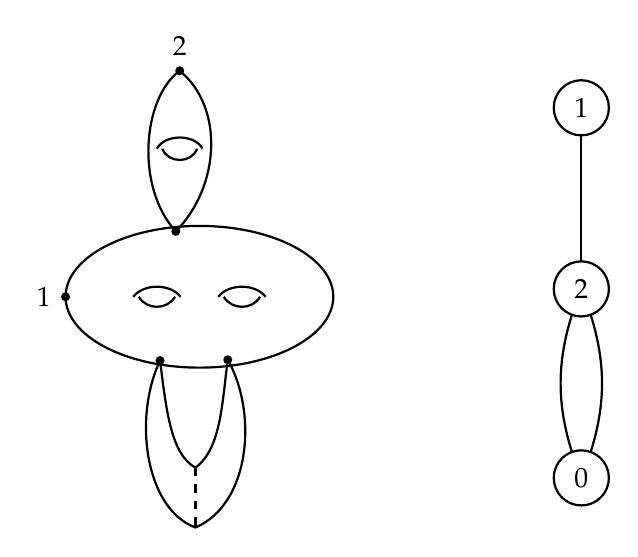
\begin{tikzpicture}[
        x=1cm,
        y=1cm,
        curve component/.style={thick},
        marked point/.style={circle,fill=black,inner sep=1.15pt},
        graph vertex/.style={
            circle,draw,thick,fill=white,minimum size=7mm,inner sep=0pt
}
    ]
        % A three-component curve with components of genera 1, 2, and 0.
        \draw[curve component] (1.5,3.65) ellipse [x radius=1.7,y radius=0.9];

        % The two handles on the genus-two component.
        \draw[curve component]
            (0.66,3.65)
            .. controls (0.79,3.82) and (1.13,3.82) .. (1.26,3.65);
        \draw[curve component]
            (0.73,3.65)
            .. controls (0.83,3.48) and (1.09,3.48) .. (1.19,3.65);
        \draw[curve component]
            (1.74,3.65)
            .. controls (1.87,3.82) and (2.21,3.82) .. (2.34,3.65);
        \draw[curve component]
            (1.81,3.65)
            .. controls (1.91,3.48) and (2.17,3.48) .. (2.27,3.65);

        % The genus-one component attached above.
        \coordinate (uppernode) at (1.2,4.48);
        \draw[curve component]
            (uppernode)
            .. controls (0.68,5.05) and (0.78,6.18) .. (1.25,6.52)
            .. controls (1.82,6.05) and (1.76,5.05) .. cycle;
        \draw[curve component]
            (0.96,5.53)
            .. controls (1.06,5.72) and (1.44,5.72) .. (1.54,5.53);
        \draw[curve component]
            (1.03,5.53)
            .. controls (1.10,5.34) and (1.40,5.34) .. (1.47,5.53);

        % The rational component attached at two nodes below.
        \coordinate (lowerleft) at (1.00,2.84);
        \coordinate (lowerright) at (1.86,2.85);
        \draw[curve component]
            (lowerleft)
            .. controls (0.65,2.10) and (0.82,0.95) .. (1.45,0.72)
            .. controls (2.15,1.02) and (2.24,2.18) .. (lowerright);
        \draw[curve component]
            (lowerleft)
            .. controls (1.08,2.20) and (1.14,1.65) .. (1.45,1.48)
            .. controls (1.78,1.72) and (1.79,2.34) .. (lowerright);
        \draw[curve component,dashed] (1.45,1.48) -- (1.45,0.72);

        % Nodes and marked points.
        \node[marked point] at (uppernode) {};
        \node[marked point] at (lowerleft) {};
        \node[marked point] at (lowerright) {};
        \node[marked point,label=left:{$1$}] at (-0.2,3.65) {};
        \node[marked point,label=above:{$2$}] at (1.25,6.52) {};

        % The dual graph: the vertex labels record the genera.
        \coordinate (vone) at (6.35,6.05);
        \coordinate (vtwo) at (6.35,3.75);
        \coordinate (vzero) at (6.35,1.35);
        \draw[curve component] (vone) -- (vtwo);
        \draw[curve component]
            (vtwo) to[out=-112,in=112] (vzero);
        \draw[curve component]
            (vtwo) to[out=-68,in=68] (vzero);
        \node[graph vertex] at (vone) {$1$};
        \node[graph vertex] at (vtwo) {$2$};
        \node[graph vertex] at (vzero) {$0$};
    \end{tikzpicture}
    \end{center}
\end{exm}

对于对数或穿孔映射穿孔\(R\)-映射
\begin{equation*}
\begin{tikzcd}
    & \mf{P} \ar{d} \\
    C \ar{ur}{f} \ar{d} \ar{r} & B \C_{\omega}^{\times} \\
    S,
\end{tikzcd}
\end{equation*}
我们将通过取整个图的关联广义锥复形来对其进行热带化。由于\(B \C_{\omega}^{\times}\)没有对数结构对数结构，我们看到的是
\begin{equation*}
\begin{tikzcd}
    \Sigma(C) \ar{d} \ar{r}{\Sigma(f)} & \Sigma(\mf{P}) = \R_{\geq 0} \\
    \Sigma(S).
\end{tikzcd}
\end{equation*}
现在假设\(S = \Spec (Q \to \C)\)是一个对数点，其中\(Q\)是一个 fs 精细幺半群尖幺半群。特别地，这意味着\(\Sigma(S) = Q_{\R}^{\vee}\)。由于所有内容都是（分段）线性的，因此只需考虑一个内部点\(t \in \Sigma(S)\)并考虑\(\Sigma(C)_t\)。

对于每条半边，我们将其视为从所附顶点指向外部，特别是这意味着一个到\(\R_{\geq 0}\)的线性映射对应于一个斜率。我们将这些称为 \textit{接触阶数}。特别是，若\(c(h) = - c(\hat{h})\)当且仅当\(h \neq \hat{h}\)通过\(\imath\)相关联时成立。对于所有\(v \in \V\)，我们还定义了 \textit{退化性}。
\[ e_v \colon Q_{\R}^{\vee} \to \R_{\geq 0} \qquad t \mapsto \Sigma(f)_t (v). \]
特别地，\(e_v \in Q\)是一个整点。

我们需要引入的下一个概念是穿孔腿。它们将被表示为
\[ \L^{\circ} = \ab\{ h \in \H \mid \Sigma(f)_t(h) \text{ 对所有 } t \in Q_{\R}^{\vee}\text{ 均有界且非平凡}\}. \] 
我们将定义在\(h \in \L^{\circ}\)上的预稳定性，使得\(0 \in \ol{\Sigma(f)_t(h)}\)，这是技术上必要的假设。在所有穿孔腿都是预稳定的假设下，我们可以定义 \textit{ 边长 } 函数
\[ \ell \colon \E \cup \L^{\circ} \to \ms{Map}(Q_{\R}^{\vee}, \R_{\geq 0}) \qquad x \mapsto \ell(x) \colon t \mapsto \ell(x)(t). \]
注意，对于边\(E\)，\(\ell(E) \in Q\)也是一个整点。对于穿孔腿，这在细分后成立。

\subsection{对数 GLSM 不变量}%
\label{sub:Log GLSM invariants}

\begin{defn}
    我们将定义 \textit{装饰热带型} 对数映射\(f\)的
    \[ \bm{\tau} = (G, c \colon \H \to \Z, \beta \colon \V \to H_2(X)). \]
\end{defn}

\begin{defn}
一个对数或穿孔映射穿孔映射\(f\)被称为 \textit{ 紧致类型 }，当且仅当
    \begin{enumerate}
\item \(\Ima \Sigma(f)_t\)对所有\(t\)有界；
\item \(f(p_h) \in 0_{\mf{P}}\)对所有接触阶为\(0\)的半边\(h\)成立。
    \end{enumerate}
\end{defn}

我们现在能够定义一个以\(\mc{R}(\mf{P}, \tau)\)为稳定穿孔\(R\)-映射的范畴，其纤维化于\(\ms{LogSch}\)范畴，后者由fs对数概形构成，并由\(\tau\)标记。

\begin{thm}[{\cite{CJR2021,CJRpunctured}}]
叠\(\mc{R}(\mf{P},\bm{\tau})\)由一个带基本（亦即最小）对数结构的固有 DM 叠表示。
\end{thm}

\begin{rmk}
如果\(\V = \ab\{v\}\)是单元素集，则我们将写为
    \[ \mc{R}_{g, c}(\mf{P}, \beta) \coloneqq \mc{R}(\mf{P}, \bm{\tau}). \]
\end{rmk}

考虑图示
\begin{equation*}
\begin{tikzcd}
    & \mf{P} \ar{d} \\
    \mc{C} \ar{ur}{f} \ar{d}{\pi} \ar{r} & B \C_{\omega}^{\times} \\
    \mc{R},
\end{tikzcd}
\end{equation*}
其中我们设定\(\mc{R} \coloneqq \mc{R}(\mf{P}, \bm{\tau})\)。然后，由完美障碍理论定义的
\[ T_{\mc{R}/\ms{Log}_{\mf{M}_G}} \to \E_{\square} = R \pi_* f^* T_{\mf{P}/B\C_{\omega}^{\times}}. \]
这里，两个切丛都指对数切复形。从完美障碍理论来看，这定义了标准的虚拟循环
\[ [\mc{R}(\mf{P}, \bm{\tau})]^{\vir}. \]
该虚拟循环的主要缺点在于它无法复现 Gromov--Witten 理论。然而，我们可以考察它与 GW 理论的差异，但为此需借助一个双有理变换。设\(Q\)为一尖幺半群。若存在非零\(c \in Q\)使得\(a+c = b\)，则称其关于\(a < b\)有偏序关系。

\begin{defn}
若存在\(e_{\max} \in \ab\{e_v \mid v \in \V \}\)使得对所有\(v \in \V\)有\(e_{\max} \geq e_v\)，则称\(f\)或\(\Sigma(f)\)具有 \textit{均匀最大退化}。
\end{defn}

\begin{rmk}
若\(f\)为紧致类型且具有均匀最大退化，则\(\Sigma(f)\)由\(e_{\max}\)一致有界。
\end{rmk}

\begin{defn}
定义\(\mc{U}(\mf{P}, \bm{\tau})\)为具有均匀最大退化的、由\(\bm{\tau}\)标记的稳定穿孔或对数\(R\)-映射的模叠。
\end{defn}

\begin{rmk}
若\(\V = \ab\{v\}\)为单元素集，则记作
    \[ \mc{U}_{g, c}(\mf{P}, \beta) \coloneqq \mc{U}(\mf{P}, \bm{\tau}). \]
若接触阶为负数，则记作
    \[ \mc{U}_{g, c}(\infty, \beta) \coloneqq \mc{U}(\mf{P}, \bm{\tau}). \]
\end{rmk}

需注意，存在两类顶点：若顶点映射至\(0\)，则至少存在一条向上指向的半边，或所有接触阶均为\(0\)（此时所有顶点均被收缩）。此类顶点称为 \textit{对数顶点}。另一类顶点不映射至\(0\)，其特征为：要么所有半边均向下指向，要么存在部分半边向上指向。此类顶点称为 \textit{\(\infty\)-顶点}。此外，紧致类型的顶点即无向上指向半边的顶点。

若忽略均匀最大退化的条件，则存在一个映射
\[ \mc{U}(\mf{P}, \bm{\tau}) \xrightarrow{F} \mc{R}(\mf{P}, \bm{\tau}) \]
这是\(\ms{LogSch}\)上的一个子范畴；但作为代数叠之间的态射，它是对数 \'etale、固有且满射的。此外，\(\mc{U}\)带有从\(\mc{R}\)拉回的典范完美障碍理论。当顶点集只有一个元素时，有
\begin{align*}
    F_* [\mc{U}_{g, c}(\mf{P}, \beta)]^{\vir} &= [\mc{R}_{g, c}(\mf{P}, \beta)]^{\vir}; \\
    F_* [\mc{U}_{g, c}(\infty, \beta)]^{\vir} &= [\mc{R}_{g, c}(\infty, \beta)]^{\vir}.
\end{align*}
在对数顶点的情况下，我们实际上有来自带 p-域的稳定映射模空间的包含关系
\begin{equation*}
\begin{tikzcd}
    \mc{U} \ar{rr}{F} & & \mc{R} \\
    & \mc{R}_{g,c}(\mf{P}^{\circ}, \beta) \ar[hookrightarrow]{ul} \ar[hookrightarrow]{ur}.
\end{tikzcd}
\end{equation*}
若将 p-域的模记为\(\mc{R}^{\circ}\)，则边界
\[ \Delta \coloneqq \mc{U} \setminus \mc{R}^{\circ} \]
是 Cartier 分割。由均匀最大退化条件，存在一个截面
\[ e_{\max} \in H^0(\bar{M}_{\mc{U}}). \]
等价于一个态射
\[ \mc{U} \to ([\A^1/\G_m], 0) \]
其将\(0\)拉回至\(\Delta\)。

我们将定义一个 \textit{超势函数} 为函数
\begin{equation*}
\begin{tikzcd}
    \mf{P}^{\circ} \ar{rr}{W} \ar{dr} && \mc{L}_{\omega} \ar{dl} \\
    & B \C_{\omega}^{\times}.
\end{tikzcd}
\end{equation*}
其 \textit{临界轨迹} 用 " 表示
\[ \on{Crit}(W) = (\d{W} = 0). \]
若\(\on{Crit}(W) \to B\C_{\omega}^{\times}\)固有，则称\(W\)具有\textit{固有临界轨迹}。

例如，若我们关注 GW 理论。令\(X\)为光滑的射影簇，\(V\)为\(X\)上的向量丛，且\(s \in H^0(V)\)。设\(Z = (s = 0)\)。则可得
\[ W \colon \mf{P}^{\circ} = V^{\vee} \boxtimes \mc{L}_{\omega} \xrightarrow{s \otimes 1_{\omega}} \mc{L}_{\omega}. \]

\begin{lem}
\(W\)的临界轨迹固有，当且仅当\(Z\)光滑且具有预期余维数。
\end{lem}

\begin{exm}
令\(X\)为点，\(V = \C\)，且\(s \neq 0\)。则\(\d{W} = s \neq 0\)，故临界轨迹为空。
\end{exm}

使用 Kiem--Li 的余截面局部化方法~\cite{KiemLi2013}，我们可以得到一个虚拟循环
\[ [\mc{R}_{g, c=n}(\mf{P}^{\circ}, \beta)]_W^{\vir}, \]
该轨迹在临界点上被支持。在 Gromov-Witten 理论中，这等于 Gromov--Witten 理论的虚拟循环，
\[ \pm [\bar{M}_{g,n}(\on{Crit}(W), \beta)]^{\vir}, \]
其符号可以显式计算。

\begin{thm}[{\cite{CJR2021,CJW2021}}]
设\(\bm{\tau}\)为紧致类型。在紧致类型设定下，
    \begin{enumerate}
        \item \(\mc{U}(\mf{P}, \bm{\tau})\)具有减少的完美障碍理论，这会产生一个减少的虚拟循环\([\mc{U}(\mf{P}, \bm{\tau})]^{\vir}\)；
        \item \(\Delta\)具有减少的完美障碍理论，这会产生一个减少的虚拟循环\([\Delta]^{\vir}\)；
        \item 在单个对数顶点的情况下，我们有\([\mc{U}_{g, c=n}(\mf{P}, \beta)]^{\on{red}} = \pm [\bar{M}_{g,n}(\on{Crit}(W), \beta)]^{\vir}\)。此外，存在公式
            \[ [\mc{U}_{g, c=n}(\mf{P}, \beta)]^{\on{red}} = [\mc{U}_{g, c=n}(\mf{P}, \beta)]^{\vir} - \tilde{r} [\Delta]^{\on{red}}, \]
            其中\(\tilde{r}\)是\(W\)沿\(\infty\)的极点阶数。
    \end{enumerate}
\end{thm}

\subsection{热带分解与有限生成性}%
\label{sub:Tropical decomposition and finite generation}

下面的热带分解及其应用出自工作草稿~\cite{CJRtropical2025}。有效不变量及其公理见~\cite{CJRpunctured}。

从现在开始，我们考虑一个更简单的设定，其中\(X\)是一个光滑射影簇，且\(V\)是\(X\)上的线丛。在此情况下，我们假设\(Z = (s = 0)\)是光滑，其亏格为\(1\)。此外，我们假设\(Z\)是一个 Calabi--Yau 三维簇。我们将考虑不变量
\[ N_{g, \beta} \coloneqq \int_{[\bar{M}_{g,0}(Z, \beta)]^{\vir}} 1 \in \Q \]
和生成级数
\[ F_g = \sum_{\beta \geq 0} N_{g, \beta} Q^{\beta} \in \Lambda \coloneqq \C \ps{Q}. \]

\begin{conj}[Yamaguchi-Yau, Alim-L\"ange {\cite{YY2004,AlimLange2007}}]
    假设\(g=0\)在镜像对称下对\(Z\)成立。那么存在一个有限生成的\(\Q\)-代数\(R \subset \Lambda\)，使得对所有\(g \geq 2\)，有\(F_g \in (I_0(q))^{2g-2} R\)。
\end{conj}

我们的主要目标如下。

\begin{thm}[{\cite{CJRtropical2025}}]
    设\(Z\)为 Fano 四维簇\(X\)中的 Calabi--Yau 三重 Calabi--Yau 三维簇奇异超曲面，且其奇数上同调为零。设\(\{\phi_j\}\)为\(H^*(X)\)的一组基，\(\ab\{\phi^j\}\)为其对偶基。那么对于所有\(g \geq 0\)，我们有
    \begin{align*}
        &F_g = (-1)^{1-g} \sum_{\tau' \in G_g'} \frac{(-1)^{\abs{\V_{\infty}}}}{\abs{\Aut(\tau')}} \cdot \prod_{E \in \E} c(E) \\
        & \cdot \sum_{j_E \mid E = \ab\{E_{\log}, E_{\infty}\} \in \E} \prod_{\substack{v \in \V_{\infty} \\ g(v)=1 \\ \H_v = \ab\{E_{\infty}\}}} c_1^{\mr{eff}}(\phi^{j_E}) \cdot \prod_{\substack{v \in \V_{\infty} \\ g(v) \geq 2}} \tilde{Q}^{\beta(v)} \cdot \exp \ab(\int_{\beta(v)} K(Q) )  \\
        & \cdot \ab(\prod_{E_{\infty} \in \H_v'}\int_{\beta(v)} \phi^{j_E}) \cdot c_{g(v), \beta(v)}^{\on{eff}} 
         \cdot \prod_{v \in \V_{\log}} \Omega_{g(v), \abs{\H_1(v)}, \abs{\H_2(v)}} (\phi_{j_E} \colon E_{\log} \in \H_1(v)).
    \end{align*}
\end{thm}

\begin{exm}
设\(Y\)为一带有对数结构的簇。此时\(\Sigma(Y)\)作为锥复形处理，我们可以考虑其边界\(\Delta_Y = \sum_{\rho \in \Sigma(Y)^1} \Delta_{\rho}\)。
\end{exm}

如果考虑\([\Delta]^{\on{red}}\)，我们应该得到类似的公式
\[ [\Delta]^{\on{red}} = \sum_{\rho \in \Sigma(\Delta)(1)} [\Delta_{\rho}]^{\on{red}}. \]
当前问题是\(\rho\)表示什么。实际上，它们参数化了刚性热带曲线。在热带化
\begin{equation*}
\begin{tikzcd}
    \Sigma(C)_{\rho} \ar{d} \ar{r} & \Sigma(\mc{C}) \ar{r}{f} \ar{d} & \R_{\geq 0} \\
    \rho \ar[hookrightarrow]{r} & \Sigma(\mc{U}),
\end{tikzcd}
\end{equation*}
中，我们看到\(f_{\rho}\)是刚性的当且仅当源热带曲线是一个二分图，其中一组顶点映射到\(e_{\max}\)，另一组顶点映射到\(0\)。

\begin{exm}
    设\(X\)为一个点，\(Z = \emptyset\)为空集。此外考虑\(g = 2, n = 0\)。那么可能的图在 ~\Cref{fig:tropgraphs} 中给出。
    \begin{figure}[htpb]
    \begin{center}
    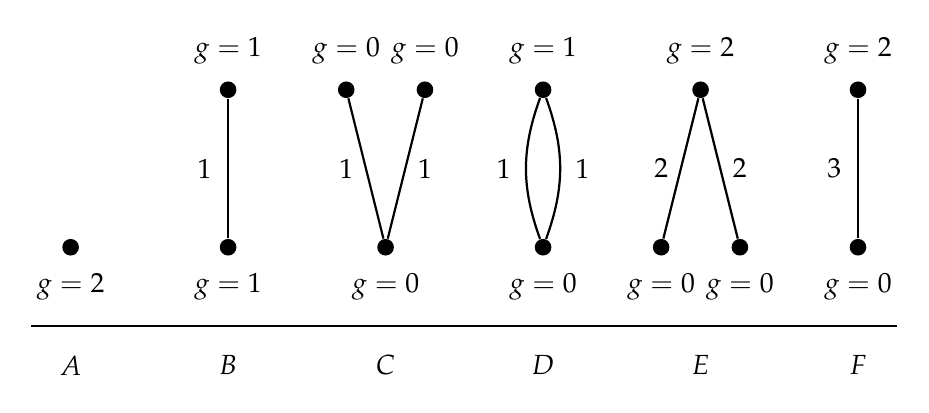
\begin{tikzpicture}[scale=1, transform shape]
        \node[fill=black,circle,minimum size=6pt,inner sep=0pt] (A) at (0,0) {};
        \node[fill=black,circle,minimum size=6pt,inner sep=0pt] (B1) at (2,0) {};
        \node[fill=black,circle,minimum size=6pt,inner sep=0pt] (B2) at (2,2) {};
        \node[fill=black,circle,minimum size=6pt,inner sep=0pt] (C1) at (4,0) {};
        \node[fill=black,circle,minimum size=6pt,inner sep=0pt] (C2) at (3.5,2) {};
        \node[fill=black,circle,minimum size=6pt,inner sep=0pt] (C3) at (4.5,2) {};
        \node[fill=black,circle,minimum size=6pt,inner sep=0pt] (D1) at (6,0) {};
        \node[fill=black,circle,minimum size=6pt,inner sep=0pt] (D2) at (6,2) {};
        \node[fill=black,circle,minimum size=6pt,inner sep=0pt] (E1) at (8,2) {};
        \node[fill=black,circle,minimum size=6pt,inner sep=0pt] (E2) at (7.5,0) {};
        \node[fill=black,circle,minimum size=6pt,inner sep=0pt] (E3) at (8.5,0) {};
        \node[fill=black,circle,minimum size=6pt,inner sep=0pt] (F1) at (10,0) {};
        \node[fill=black,circle,minimum size=6pt,inner sep=0pt] (F2) at (10,2) {};
        \draw[-,thick] (B1) -- (B2);
        \draw[-,thick] (C2) -- (C1) -- (C3);
        \draw[-,thick] (D1) edge[bend left=20] (D2);
        \draw[-,thick] (D2) edge[bend left=20] (D1);
        \draw[-,thick] (E2) -- (E1) -- (E3);
        \draw[-,thick] (F1) -- (F2);
        \node at (0,-0.5) {$g=2$};
        \node at (2,-0.5) {$g=1$};
        \node at (4,-0.5) {$g=0$};
        \node at (6,-0.5) {$g=0$};
        \node at (7.5,-0.5) {$g=0$};
        \node at (8.5,-0.5) {$g=0$};
        \node at (10,-0.5) {$g=0$};
        \node at (2,2.5) {$g=1$};
        \node at (3.5,2.5) {$g=0$};
        \node at (4.5,2.5) {$g=0$};
        \node at (6,2.5) {$g=1$};
        \node at (8,2.5) {$g=2$};
        \node at (10,2.5) {$g=2$};
        \draw[-,thick] (-0.5,-1) -- (10.5,-1);
        \node at (0,-1.5) {$A$};
        \node at (2,-1.5) {$B$};
        \node at (4,-1.5) {$C$};
        \node at (6,-1.5) {$D$};
        \node at (8,-1.5) {$E$};
        \node at (10,-1.5) {$F$};
        \node at (1.7,1) {$1$};
        \node at (3.5,1) {$1$};
        \node at (4.5,1) {$1$};
        \node at (5.5,1) {$1$};
        \node at (6.5,1) {$1$};
        \node at (7.5,1) {$2$};
        \node at (8.5,1) {$2$};
        \node at (9.7,1) {$3$};
    \end{tikzpicture}
    \end{center}
        \caption{当$X = \mr{pt}$、\(Z = \emptyset\)、$g=2$时的热带型。}%
    \label{fig:tropgraphs}
    \end{figure}
\end{exm}

\begin{thm}[热带量子 Lefschetz {\cite{CJRtropical2025}}]
    设\(X\)和\(Z\)如前所述。对于任意\(\beta \in H_2(X)\)，任意\(\alpha_1, \ldots, \alpha_n \in H^*(X)\)，以及任意\(k_1, \ldots, k_n \in \N\)，我们有
    \begin{align*}
        \int_{[\bar{M}_{g,n}(Z,\beta)]^{\vir}} \prod_{j=1}^n \ev_j^* (\alpha_j) \psi^{k_j}={}& (-1)^{1-g+\beta \cdot Z} \cdot \sum_{\tau \vdash (g,n,\beta)} \frac{(-1)^{\abs{\V_{\infty}}}}{\abs{\Aut(\tau)}} \cdot \prod_{E \in \E} c(E) \\
        & \cdot \sum_{\ab\{j_E \mid E = \ab\{E_{\log}, E_{\infty}\}\}}  \prod_{v \in \V_{\infty}} \int_{[\mc{U}_v]^{\on{red}}} \prod_{E_{\infty} \in \H_v} \ev_{E_{\infty}}^* \phi^{j_E}  \\
        &  \cdot \prod_{v \in \V_{\log}} \int_{[\mc{R}_v]^{\vir}} \prod_{E_{\log}} \ev_{E_{\log}}^* (\phi_{j_E}) \cdot \prod_{h \in \L_v} \ev_h^* \alpha_h \cdot \psi_h^{k_h} .
    \end{align*}
\end{thm}

\begin{rmk}
文献~\cite{CJRlocalization} 还预告了一个虚拟局部化公式，该公式可应用于简化理论（仅包含 R-环面作用）或规范理论（可应用于环境空间的全部自同构）。
\end{rmk}

现在考虑一个\(\infty\)-顶点。设\(\tau_v = (g, c, \beta)\)，且设\(\mc{U}_v = \mc{U}_{g,c}(\infty, \beta)\)。则第一项计算为
\begin{align*}
    \on{red}\dim \mc{U}_v &= \chi(f^* T_{\mf{P}/B \C^{\times}_{\omega}}) + 1 + \on{trop}\dim  \\
    &= \vir\dim \bar{M}_{g,n}(Z, \beta) + \sum_{h \in \H } (c(h) + 1),
\end{align*}
其中热带维数为\(3g-4+n\)。注意所有接触阶均为负数，因此第二项至多为零。特别地，我们已证明
\begin{cor}[{\cite{CJRpunctured}}]
若\(\vir\dim \bar{M}_{g,n}(Z,\beta) < 0\)，则\([\mc{U}_v]^{\on{red}} = 0\)。
\end{cor}
我们还存在一个 \textit{ 平衡条件 }，其表述为
\begin{equation}\label{eqn:balancing condition}
    \sum_{h \in \H} c(h) = \deg f^* \mc{O}(\infty) = \int_{\beta} c_1(V) - (2g-2+n).
\end{equation}
可重写为
\[ 0 \geq \sum_{h \in \H} (c(h)+1) = \int_{\beta} c_1(V) - (2g-2). \]
\begin{prop}[{\cite{CJRpunctured}}]
我们观察到，以下情况下不存在\(\infty\)-顶点：
    \begin{enumerate}
\item 我们有\(g = 0\)且\(V\)为 nef；
\item 我们有\(g=1\)且\(V\)为 ample，除非\(\beta = 0\)且所有\(c(h) = -1\)。
    \end{enumerate}
\end{prop}

\begin{defn}
一个标记是 \textit{ 单位 }，当且仅当其接触阶为\(-1\)。
\end{defn}

\begin{notn}
我们将单位扇区记为\(\1\)，并记\(\tau_{v+\1} = (g, c+\1, \beta)\)，\(\mc{U}_{v+\1} = \mc{U}_{g, c+\1}(\infty, \beta)\)以及\(\mc{R}_{v+\1} = \mc{R}_{g, c+\1}(\infty, \beta)\)。
\end{notn}

\begin{thm}[{\cite[定理~1.16--1.17]{CJRpunctured}}]\leavevmode
    \begin{enumerate}
\item 存在一个映射\(F_{\1} \colon \mc{U}_{v+\1} \xrightarrow{s} \mc{C}^{\circ} \xrightarrow{\pi} \mc{U}_v\)，其中\(s\)为 birational；
\item 我们有减少的虚拟循环的等式\(s_* [\mc{U}_{v+\1}]^{\on{red}} = \pi^* [\mc{U}_v]^{\on{red}}\)；
\item 若\(D\)是\(X\)上的素子，则\(F_{\1 *} (\ev_{\1}^* D \cap [\mc{U}_{v+\1}]^{\on{red}}) = \ab(\int_{\beta} D) [\mc{U}_v]^{\on{red}}\)；
\item 考虑以下图示
            \begin{equation*}
            \begin{tikzcd}
                \mc{U}_{v+\1} \ar{r}{F} \ar{d}[swap]{F_{\1}} & \bar{M}_{g,n+1} \ar{d}[swap]{p} \\
                \mc{U}_v \ar{r}{F} & \bar{M}_{g,n}.
            \end{tikzcd}
            \end{equation*}
则\(F_* [\mc{U}_{v+\1}]^{\on{red}} = p^* F_* [\mc{U}_v]^{\on{red}}\)。
    \end{enumerate}
\end{thm}

\begin{exm}
    考虑\(g = 1\)的情形，且\(Z_d \subset X = \P^N\)为一个超曲面。我们只需考虑所有\(h \in \H\)下的\(\beta = 0\)和\(c(h) = -1\)，此时可以看到
    \[ \prod_h \ev_h^* \alpha_h \cdot [\mc{U}_{1,c}(\infty,\beta)]^{\mr{red}} = \ev_{h^{\star}}^* \ab(\prod_h \alpha_h) \cap [\mc{U}_{1,\1}(\infty,\beta)]^{\on{red}}. \]
\end{exm}

\begin{prop}[{\cite{CJRpunctured}}]
事实上，我们有
    \[ \mc{U}_{1,\1}(\infty, 0) \simeq \mc{R}_{1,\1}(\infty, 0) \]
且等式
    \[ [\mc{U}_{1,\1}(\infty, 0)]^{\on{red}} = c_{\dim X} \ab(\mc{H}^{\vee} \boxtimes T_{\mf{P}/B\C_{\omega}^{\times}} + \mc{O} - V). \]
\end{prop}

\begin{exm}
现在考虑五次三维簇\(Z_5 \subset \P^4\)。则我们观察到\(\on{red}\dim \mc{U}_v = \sum_{h \in \H} (c(h)+2)\)。单位公理将问题简化为\(c(h) \leq -2\)的情形。现在需要确定若所有\(c(h) = -2\)，即等价于求解可能的\(\beta\)数量。平衡条件表明
    \begin{align*}
        \sum_{h \in \H} c(h) &= \int_{\beta} c_1(V) - (2g-2+n) \\
        &= 5\beta - (2g-2+n),
    \end{align*}
    这意味着\(0 \geq \sum (c(h)+1) = 5\beta - (2g-2)\)，因而\(\beta \leq \frac{2g-2}{5}\)。\footnote{这正是有限生成性、全纯反常方程、orbifold 正则性与 conifold 间隙条件所预言的未知数个数。}
\end{exm}

\begin{conj}[Janda {\cite[猜想~1.6]{CJRtropical2025}}]\leavevmode
    \begin{enumerate}
        \item 我们有\(K(Q) = \log I_0(q) \cdot c_1(K_X^{\vee}) - \frac{I_1}{I_0}\)。\\
\item 规范理论满足\(\Omega \in I_0(q)^{2g-2+2n_1 + 3 n_2} \cdot R\)。
    \end{enumerate}
\end{conj}

\begin{cor}[{\cite[定理~1.7]{CJRtropical2025}}]
上述关于\((X, V)\)的猜想蕴含了对\(Z\)的 Yamaguchi-Yau 有限生成性。
\end{cor}

\section{五次三维簇高亏格 GW 不变量的结构（郭帅）}%
\label{sec:Structure of higher-genus GW invariants of the quintic (郭帅)}

\subsection{问题}%
\label{sub:The problem (Guo)}

考虑五次三维簇\(X = X_5 \subset \P^4\)。我们要问：\(X\)中包含多少条亏格为\(g\)、次数为\(d\)的曲线？亏格零时，答案的前几项是
\[ 2875, \qquad 609250, \qquad 317206375, \qquad \ldots \]

由于\(X\)是 Calabi--Yau 三维簇，模空间\(\Mbar_{g,n}(X,\beta)\)的虚维数为零；弦方程还给出\(\ab<\1, \gamma_2, \ldots, \gamma_n>_{g,n,\beta} = 0\)，唯一的例外是\((g,n,\beta) = (0,3,0)\)。因此定义主不变量
\[ N_{g,\beta} \coloneqq \ab<>_{g,0,\beta} = \int_{[\Mbar_g(X,\beta)]^{\vir}} 1 \]
并把它们收集成生成级数
\[ F_g(Q) \coloneqq \sum_{\beta \text{ 有效}} N_{g,\beta}Q^{\beta}. \]

不变量\(N_{g,\beta}\)是有理数；真正希望得到的整数是 BPS 不变量\(n_{g,\beta}\)。后者由\(F_g\)的正次数部分\(F_g^+\)通过多重覆盖变换定义：
\[ \sum_{g \geq 0} F_g^+(Q)\lambda^{2g-2} = \sum_{\substack{g \geq 0 \\ \beta > 0}} n_{g,\beta} \sum_{k \geq 1} \frac{1}{k} \ab(2 \sin \frac{k\lambda}{2})^{2g-2}Q^{k\beta}. \]
只有\(n_{g,\beta}\)才预期为整数；上面列出的数正是\(n_{0,d}\)。

\begin{table}[htpb]
    \centering
    \caption{五次三维簇的首批 BPS 不变量\(n_{g,d}\)}
    \label{tab:quinticbps}
    \begin{tabular}{crrrrr}
        \toprule
        \(g\) & \(d=1\) & \(d=2\) & \(d=3\) & \(d=4\) & \(d=5\) \\
        \midrule
        0 & 2875 & 609250 & 317206375 & 242467530000 & 229305888887625 \\
        1 & 0 & 0 & 609250 & 3721431625 & 12129909700200 \\
        2 & 0 & 0 & 0 & 534750 & 75478987900 \\
        3 & 0 & 0 & 0 & 8625 & \(-15663750\) \\
        4 & 0 & 0 & 0 & 0 & 49250 \\
        5 & 0 & 0 & 0 & 0 & 1100 \\
        6 & 0 & 0 & 0 & 0 & 10 \\
        7 & 0 & 0 & 0 & 0 & 0 \\
        \bottomrule
    \end{tabular}
\end{table}

从~\Cref{tab:quinticbps}可以看出，每一列最终都归零。这就是 Castelnuovo 界：对五次三维簇，一旦\(g > \frac{d^2+5d+10}{10}\)，便有\(n_{g,d}=0\)；这一结论由刘治宇与阮勇斌~\cite{LiuRuanCastelnuovo} 证明。表中各项的整性则是 Gopakumar--Vafa 猜想的内容，由 Ionel--Parker~\cite{IonelParker2018} 证明。

在亏格零时，Candelas、de la Ossa、Green 与 Parkes 利用镜像上的周期积分计算了\(F_0\)，这正是~\Cref{sub:Enumerative mirror symmetry in genus zero}讨论的内容。在高亏格时，Bershadsky、Cecotti、Ooguri 与 Vafa 给出递归关系，可以由所有\(h<g\)的\(F_h\)确定\(F_g\)，但会留下有限多个未知常数。我们的目标是解释对数 GLSM 如何消除这一全纯模糊性。

\subsection{亏格零与 B 模型的多项式结构}%
\label{sub:Genus zero and the polynomial structure of the B-model}

回顾~\Cref{sub:Enumerative mirror symmetry in genus zero}，五次三维簇的\(I\)-函数为
\[
    I(q,z) = z\sum_{d \geq 0} q^{H/z+d} \frac{\prod_{m=1}^{5d}(5H+mz)}{\prod_{m=1}^d (H+mz)^5} = I_0 z + I_1 H + I_2 \frac{H^2}{z} + I_3 \frac{H^3}{z^2},
\]
其各分量都被 Picard--Fuchs 算子
\[ D^4 - 5q(5D+1)(5D+2)(5D+3)(5D+4), \qquad D = q \odv{}{q} \]
所湮灭。
若我们记\(J_k = I_k/I_0\)和\(\frac{I_1}{I_0} = \log q + \tau(q)\)，则\(Q = e^{I_1/I_0} = qe^{\tau(q)} = q + O(q^2)\)，此时亏格零镜像定理表明
\[ F_0(Q) = \frac{5}{2}\ab(J_1 J_2 - J_3). \]

对我们而言，把五次三维簇的公式放进一般的镜像对称框架更为有用。设\(\mc{X} = \ab\{(X,\omega)\}\)为一族 Calabi--Yau 三维簇，其 Kähler 模空间为\(\mc{M} \ni Q = e^{2\pi i \omega}\)；设\(\mc{X}^{\vee} = \ab\{(X^{\vee},J)\}\)为镜像族，其复模空间为\(\mc{M}^{\vee} \ni q\)。Picard--Fuchs 方程的解是\(X^{\vee}\)上的周期，并组合成
\[ I(z) = zI_0\varphi_0 + I_1 + I_2 z^{-1} + I_3 z^{-2}, \]
它位于\(z\varphi_0, \varphi_{\alpha}, \varphi^{\alpha}z^{-1}, \varphi^0 z^{-2}\)的张成空间中。这里\(I_1 = \sum_{\alpha} I_1^{\alpha}\varphi_{\alpha}\)、\(I_2 = \sum_{\alpha} I_{2,\alpha}\varphi^{\alpha}\)、\(I_3 = I_{3,0}\varphi^0\)，镜像映射仍为\(Q = e^{I_1/I_0} = qe^{\tau(q)}\)。

五次三维簇的复模直线上有三个特殊点：大复结构点\(q=0\)、conifold 点\(q = 5^{-5}\)（有一个周期在此消失），以及 orbifold（或 Landau--Ginzburg）点\(q = \infty\)。镜像映射在\(q=0\)附近定义，其展开给出 Gromov--Witten 不变量；在高亏格时，我们还要在另外两个点施加边界条件。

现在，我们用三点函数重新表述镜像定理。在\(\mc{M}^{\vee}\)上选取局部坐标\(q_i\)，令\(\ab\{\phi_i\}\)为 A 侧对应的基，定义
\[ C^A_{ijk}(Q) \coloneqq I_0^2 \ab<\phi_i, \phi_j, \phi_k>^X_{0,3}, \qquad C^B_{ijk}(q) \coloneqq \int_{X^{\vee}} \partial_i \partial_j \partial_k \Omega \wedge \Omega. \]

\begin{thm}[镜像定理 {\cite{Givental1998,LLY1997}}]
我们有\(C^A_{ijk}(Q(q)) = C^B_{ijk}(q)\)。此外，\(C^B_{ijk} \in \Delta^{-1}\Q[q]\)，因此它在\(\mc{M}^{\vee}\)上是全局定义的亚纯函数，奇点仅沿判别式分布。
\end{thm}

特别是，在乘以\(I_0\)的适当幂次并应用镜像映射后，一个亏格为零的生成函数变为\(q\)的有理函数，且极点仅出现在判别式处。因此，它由有限多个系数唯一确定。

\begin{exm}
对于超平面基中的五次三维簇，
    \[ C_{111} = \frac{5}{1-5^5 q}. \]
\end{exm}

\begin{exm}
对于\(X = X_{3,3} \subset \P^2 \times \P^2\)，Yukawa 耦合为
    \begin{align*}
        C_{111} &= \frac{3^4 q_1 (2+3^3q_1+3^3q_2)}{\Delta}, & C_{222} &= \frac{3^4 q_2(2+3^3q_1+3^3q_2)}{\Delta}, \\
        C_{112} &= \frac{(1-3^3q_1-3^3q_2)(1+2\cdot 3^3 q_1 - 3^3 q_2)}{\Delta}, \\
        C_{122} &= \frac{(1-3^3q_1-3^3q_2)(1-3^3q_1+2\cdot3^3q_2)}{\Delta},
    \end{align*}
其中
    \[ \Delta = 1 - 3\cdot3^3(q_1+q_2) + 3\cdot3^6(q_1^2 - 7q_1q_2+q_2^2) - 3^9(q_1+q_2)^3. \]
\end{exm}

在高亏格情况下，我们期望满足\(f^A_{g,i}\)的标准化势函数
\[ f^A_{g,i}(Q(q)) = f^B_{g,i}(q) \in \Delta^{-(2g-2+n)}\Q[q], \]
其中右侧由图的求和计算。

\subsection{BCOV Feynman 规则}%
\label{sub:The BCOV Feynman rule}

Feynman 规则与全纯反常方程见~\cite{BCOV1994}。对于五次三维簇，张怀良、郭帅与李骏在~\cite{CGL2021} 中证明了多项式性，在~\cite{CGL2026} 中证明了 Feynman 规则。

我们现在讨论 BCOV 递归作为 Feynman 规则。它来源于一个有限维模型，用于描述辛变换的量子化，如 ~\Cref{sub:Operator formalism and geometric quantization} 所示。设\(\mc{H} = \mc{H}^- \oplus \mc{H}^+ \subset \mc{H}_{\infty}\)为辛结构，其维度为\(d+1 = \dim \mc{H}^+ = \dim \mc{H}^-\)，并定义
\[ R = \begin{pmatrix} A & B \\ C & D \end{pmatrix} \in \End \mc{H}, \qquad \mc{Q}(\mbf{x},\bp) = (\bp, D^{-1}\mbf{x}) - \frac{1}{2}(\bp, D^{-1}C\bp). \]
给定总势\(F(\hbar, \mbf{x})\)，形式地把变换后的势定义为高斯积分
\[ f(\hbar, \mbf{x}) \coloneqq (\wh{R}F)(\hbar,\mbf{x}) = \ln \int e^{\hbar^{-1}(\mc{Q}(\mbf{x},\bp') - \mbf{x}'\bp') + F(\hbar,\mbf{x}')}\d{\mbf{x}'}\d{\bp'}. \]
通过驻点展开得到图的求和。此处，\(D^{-1}C\)为每条边提供传播子，\(F\)为顶点提供贡献。

对于 Calabi--Yau 三维簇，传播子根据指标数量分别表示为\(S^{\varphi\varphi}\)、\(S^{\varphi}\)和\(S\)，而顶点则由标准化的 A-模关联子给出
\[ P^A_{g,n}(Q) = I_0^{2-2g}\ab<\phi_1, \ldots, \phi_n>^X_{g,n}. \]
需注意，这些与解量子微分方程的算子\(S_{\tau}(z)\)无关，后者将在后续出现。

\begin{exm}
    对于亏格为二且无标记的五次三维簇，Feynman 规则表述为
    \begin{align*}
        f_2^B ={}& P_2 + \frac{1}{2}S^{\varphi\varphi}P_{1,1}^2 + \frac{1}{2}S^{\varphi\varphi}P_{1,2} + (S^{\varphi\varphi})^2 P_{1,1} + \frac{1}{8}(S^{\varphi\varphi})^2 P_{0,4} \\
        &+ \frac{1}{8}(S^{\varphi\varphi})^3 + \frac{1}{12}(S^{\varphi\varphi})^3 + \frac{\chi}{24}S^{\varphi}P_{1,1} + \frac{1}{2}\frac{\chi}{24}S^{\varphi}S^{\varphi\varphi} \\
        &+ \frac{1}{2}\frac{\chi}{24}\ab(\frac{\chi}{24}-1)S,
    \end{align*}
其中\(\chi = \chi(X_5) = -200\)。这是传播子的三次多项式。
\end{exm}

如~\Cref{sub:R-matrix action}所示，这可以理解为对稳定图求和。顶点\(v\)贡献低亏格关联子\(P_{g_v, \on{val}(v)}\)；内边通过传播子收缩两个插入；腿记录其余插入。每个图的权重为\(\frac{1}{\ab|\Aut \Gamma|}\)。照例，
\[ g(\Gamma) = h^1(\Gamma) + \sum_v g_v, \qquad 2g_v - 2 + \on{val}(v) > 0, \]
而\(f_g^B\)就是所有亏格为\(g\)的稳定图贡献之和。

\subsection{全纯反常方程}%
\label{sub:The holomorphic anomaly equation}

现在把递归关系改写为微分方程。B 模型振幅\(\mc{F}_g(z,\bar{z})\)并非全纯；当\(g \geq 2\)时，它的非全纯性由下式控制：
\[ \partial_{\bar{i}} \mc{F}_g = \frac{1}{2}\bar{C}_{\bar{i}}^{jk}\ab( D_j D_k \mc{F}_{g-1} + \sum_{r=1}^{g-1} D_j \mc{F}_r D_k \mc{F}_{g-r} ). \]
其中，\(C_{ijk}\)是Yukawa耦合，\(\bar{C}_{\bar{i}}^{jk}\)由\(\bar{C}_{\bar{i}\bar{j}\bar{k}}\)通过Weil-Petersson度量提升两个指标得到，\(D_j\)是Hodge模线丛的恰当导数。等式右侧的两项是\(\Mbar_g\)的两个边界分量，即一个非分离点和一个分离点。\(\frac{1}{2}\)会遗忘两个分支的顺序。

若我们选择局部\(\bar{\partial}\)-原函数
\[ \partial_{\bar{i}}S^{jk} = \bar{C}_{\bar{i}}^{jk}, \qquad \partial_{\bar{i}}S^j = G_{i\bar{\ell}}S^{\ell j}, \qquad \partial_{\bar{i}}S = G_{i\bar{\ell}}S^{\ell}, \]
使得模全纯项后，奇点方程退化为多项式偏微分方程
\[ \pdv{\mc{F}_g}{S^{jk}} = \frac{1}{2}\ab( D_jD_k \mc{F}_{g-1} + \sum_{r=1}^{g-1} D_j \mc{F}_r D_k \mc{F}_{g-r} ). \]
这些传播子仅在全纯张量意义下定义，这种自由度正是全纯模糊性的来源。

\begin{rmk}
在五次三维簇的单参数归一化变量下，其表达式为
    \[ -\partial_0 P_g = \frac{1}{2}P_{g-1,2} + \frac{1}{2}\sum_{r=1}^{g-1}P_{r,1}P_{g-r,1}, \qquad -\partial_1 P_g = 0. \]
\end{rmk}

要理解图求和为何满足该方程，请注意在未标记的势中，非全纯生成元仅出现在边因子中。沿传播方向的导数因此会选择一条边并将其截断。两个半边变为结果中低-亏格顶点上的标记，而协变导数则通过除子方程与这些标记对应。我们通过截断一个环得到\(P_{g-1,2}\)，通过截断一条分离边得到\(P_{g_1,1}P_{g_2,1}\)。

\begin{rmk}
    为明确起见，此蕴含关系仅为单向。BCOV 图规则（亏格）蕴含异常方程，但异常方程本身并不唯一确定该图规则。为了恢复相同的解，我们还需结合传播子约定、边界条件顶点数据。
\end{rmk}

若已知所有亏格低阶顶点，则右端项已知，从而可对非全纯生成元进行积分，得到
\[ P_g = P_g^{\mr{particular}} + f_g(Y), \]
其中有限生成性给出全纯模糊性
\[ f_g(Y) = P_g|_{A = B_1 = B_2 = B_3 = 0} = \sum_{i=0}^{3g-3}a_{i,g}Y^i, \qquad Y = (1-5^5q)^{-1}. \]
因此，全纯反常方程在每个亏格仍留下\(3g-2\)个未知系数。

\begin{rmk}
对于五次三维簇，度零数据与 orbifold 正则性共同消去\(\ceil{\frac{3g-3}{5}}+1\)个自由度，而 conifold 间隙再给出\(2g-2\)个条件。因此
    \[ 3g-2 - \ab(\ceil*{\frac{3g-3}{5}}+1) - (2g-2) = \floor*{\frac{2g-2}{5}} \]
    参数保持不变，且确实是新的有效不变量。这正是\(\infty\)个顶点未知数，与 ~\Cref{eqn:balancing condition} 预测一致，即满足\(\beta \leq \frac{2g-2}{5}\)的\(\beta\)的数量。
\end{rmk}

由此得到物理学家提出的猜想性算法：结合 BCOV Feynman 规则、Landau--Ginzburg 点的 orbifold 正则性（它是 LG/CY 对应的一种形式；对五次三维簇，郭帅、阮勇斌与 Janda 的相关工作仍在进行）以及 conifold 间隙条件。还可以再加入 Gopakumar--Vafa 整性与 Castelnuovo 界。

\subsection{四种理论}%
\label{sub:Four theories}

回顾~\Cref{sec:Log GLSM (陈琪乐)}，对数 GLSM 带有两个虚拟循环。约化循环恢复五次三维簇的 Gromov--Witten 理论；典范等变循环则有一个单位根特化，它是半单的，因而可用 Givental--Teleman 理论计算。双分图求和
\[ \Omega^{\mr{GW}}_{g,n} = \sum_{\Gamma \text{ 二部}} \frac{1}{\ab|\Aut \Gamma|} \ab( \prod_{v \in V_{\infty}(\Gamma)} c^{\mr{eff}}_{g_v,\beta_v}) \Cont^{\mr{can}}_{\Gamma} \]
用后者表示前者；其中\(\infty\)-顶点带有有效不变量\(c^{\mr{eff}}_{g,\beta}\)。把这些不变量替换为形式参数\(\mbf{C} = \ab\{c_{g,\beta}\}\)，便得到\textit{扩展\(\mbf{C}\)族}；其顶点数据来自 MSP 与橡胶对数 GLSM 理论。

我们将考虑以下四种理论。
\begin{itemize}
    \item \textit{\(t\)-扭曲几何理论}令\(\lambda_i = 0\)，并保留辅助权重\(t\)。它同时有稳定映射与稳定商两个版本；稳定商版本给出下述亏格二局部化公式。
    \item \textit{形式五次三维簇}，也就是形式\(\lambda\)-扭曲理论，令\(t = 0\)且\(\lambda_i = \zeta_5^i \lambda\)。它是半单 CohFT，因而具有通用且可计算的\(R\)-矩阵。
    \item \textit{扩展\(\mbf{C}\)族}介于上述理论之间，其双分图同时含有形式顶点与 MSP 顶点。
    \item \textit{五次三维簇的 Gromov--Witten 理论}由\(\mbf{C} = \mbf{C}^{\mr{eff}}\)和\(\lambda \to 0\)得到；这正是我们要计算的理论。
\end{itemize}

\begin{warn}
    在高亏格中，\(t^0\)系数的\(t\)扭稳定商理论并非\(\lambda^0\)系数的形式\(\lambda\)扭理论。
\end{warn}

\subsection{形式五次三维簇}%
\label{sub:The formal quintic}

形式五次三维簇及其全纯反常方程见~\cite{LhoPandharipande2019}；与扩展理论的比较见~\cite{GJRstructure}。

设\(E = \mc{O}_{\P^4}(5)\)与\(\pi \colon \mc{C} \to \Mbar_{g,n}(\P^4,d)\)为通用曲线。\(t\)扭态循环为
\[ e(R\pi_* f^* E \otimes [1]) \cap [\Mbar_{g,n}(\P^4,d)]^{\vir}, \]
其中\([1]\)具有等变第一陈类\(t\)。若从完全的\((\C^{\times})^5\)-等变周期出发，则形式五次三维簇对应于单位根的特殊化
\[ [\Mbar_{g,n}(\P^4,d)]^{\vir,\lambda} \coloneqq \ab( e(R\pi_*f^*E \otimes [1]) \cap [\Mbar_{g,n}(\P^4,d)]^{\vir}_{(\C^{\times})^5})\Big|_{t=0, \; \lambda_i = \zeta_5^i \lambda}, \]
其中\(\zeta_5 = e^{2\pi i/5}\)。关系\(H^5 = \lambda^5\)使量子乘积通常半单，同时保留\(\lambda\)作为参数。

态空间、单位元与配对由
\[ \mc{H}_{\lambda} = \Q(\lambda)[H]/(H^5-\lambda^5), \quad \1 = 1, \quad (\gamma_1,\gamma_2)^{\lambda} = \int_{\P^4, (\C^{\times})^5} e(\mc{O}(5))\gamma_1\gamma_2 \Big|_{\lambda_i = \zeta_5^i\lambda}, \]
给出，CohFT 类为
\[ \Omega^{\lambda}_{g,n}(\gamma_1, \ldots, \gamma_n) = \sum_{d \geq 0} q^d \rho_* \ab( \prod_{i=1}^n \ev_i^*(\gamma_i) \cap [\Mbar_{g,n}(\P^4,d)]^{\vir,\lambda}), \]
其中\(\rho\)忽略映射并稳定定义域。若通过\(\tau(q)H\)位移，且满足\(\tau(q) = I^{\lambda}_1(q)/I^{\lambda}_0(q)\)，则位移后的理论\(\Omega^{\lambda,\tau}\)为半单。在扩展标量至\(\Q(\zeta_5,\lambda)\)后，幂等基满足
\[ \omega^{\lambda}_{g,n}(e_{\alpha_1}, \ldots, e_{\alpha_n}) = \sum_{\alpha}\Delta_{\alpha}^{g-1}\prod_i \delta_{\alpha,\alpha_i}. \]
则 ~\Cref{thm:teleman} 给出
\[ \Omega^{\lambda,\tau}_{g,n} = \sum_{\Gamma \in G_{g,n}} \frac{1}{\ab|\Aut\Gamma|}\iota_* \Cont_{\Gamma} \]
带 ~\Cref{sub:R-matrix action} 装饰。携带\(\gamma\)的腿获得\(R^{-1}(\bar{\psi})\gamma\)，边获得
\[ V_R(z_1,z_2) = \frac{\sum_{\alpha} e_{\alpha}\otimes e^{\alpha} - \sum_{\alpha} R^{-1}(z_1)e_{\alpha} \otimes R^{-1}(z_2)e^{\alpha}}{z_1+z_2}, \]
顶点获得拓扑场论\(\omega\)，缺失的保单位部分通过\(T(z) = z(\1 - R^{-1}(z)\1)\)插入遗忘标记处。

\begin{rmk}
我们发现边因子无极点。设定\(z_2 = -z_1\)并利用以\(R^{-1}(z) = R^*(-z)\)形式表达的辛条件，分子消失。因此，其可被\(z_1+z_2\)整除，且\(V_R\)是两个余切线变量的幂级数。\(z_1^p z_2^q\)的系数位于带\(\bar{\psi}_1^p \bar{\psi}_2^q\)的节点上，与相邻拓扑场论张量收缩后，将分支粘合。
\end{rmk}

\subsection{如何计算\(R\)-矩阵}%
\label{sub:How to compute the R-matrix (Guo)}

为计算\(R\)-矩阵，先从等变\(I\)-函数出发：
\[ I^{\lambda}(q,z) = z\sum_{d\geq0}q^d \frac{\prod_{m=1}^{5d}(5H+mz)}{\prod_{m=1}^d ((H+mz)^5 - \lambda^5)} = zI_0 + I_1^{\lambda}H + z^{-1}I_2^{\lambda}H^2 + \cdots. \]
由于\(H\)的系数与\(\lambda\)无关，\(I_1^{\lambda} = I_1 - I_0 \log q\)以及镜像位移\(\tau(q) = I_1^{\lambda}(q)/I_0(q)\)都不含对数项。设
\[ D = q\odv{}{q}, \qquad Y = (1-5^5q)^{-1}, \qquad L = Y^{1/5} \]
并引入基
\[ \phi_k = I_{1,1}\cdots I_{k,k}H^k, \qquad \bar{\phi}_k = I_0 L^{-k-1}\phi_k, \]
其中对角线 Birkhoff 因子由递归定义
\[ I_{p,0} = I_p, \qquad I_{p,r} = \frac{I_{p-1,r-1}}{I_{r-1,r-1}} + D \ab( \frac{I_{p,r-1}}{I_{r-1,r-1}}), \quad 1 \leq r \leq p, \]
因此，特别地，\(I_{1,1} = 1+D\tau\)。恒等元和典范坐标由下式给出
\[ e_{\alpha} = \frac{1}{5}\sum_{i=0}^4 h_{\alpha}^{-i}\frac{\phi_i}{L^i}, \qquad u_{\alpha} = h_{\alpha}\int_0^q (L(s)-1)\frac{\d{s}}{s}, \qquad h_{\alpha} = \zeta_5^{\alpha}\lambda. \]

我们将使用量子微分方程来确定\(R\)-矩阵对\(q\)的依赖性。基本解满足
\[ zDS_{\tau}(z) + S_{\tau}(z)H = M_{\tau}S_{\tau}(z), \qquad M_{\tau} = \dot{\tau}\star, \quad \dot{\tau} \coloneqq (1+D\tau)H = I_{1,1}H, \]
在归一化的标准方向\(\alpha\)上，静止相渐近展开给出
\[ (S_{\tau})_{i\bar{\alpha}}(z)C_{\alpha}(z)^{-1} = e^{u_{\alpha}/z}R_{i\bar{\alpha}}(z), \]
因此
\[ (zD+h_{\alpha}L)R_{i\bar{\alpha}} = \sum_j (M_{\tau})_i^j R_{j\bar{\alpha}}. \]
此处，\(C_{\alpha}(z)\)是\(q=0\)量子 Riemann-Roch（等价于 Gamma 函数）因子，与对称条件结合后，确定了微分方程无法观测的常数。如 ~\Cref{sub:How to compute the R-matrix} 结尾所述，微分方程给出递归关系和初始条件，而振荡积分提供初始条件。

写\(R(z) = \mr{Id} + R_1 z + R_2 z^2 + \cdots\)。利用上述方程，可以由前面的系数依次确定每个\(R_{k+1}\)。五次三维簇之所以可处理，有两个原因。第一，单位根基分成五个扇区，而模\(5\)的电荷规则使每一行只允许一种余数模式，所以大多数矩阵元在计算开始前就已经为零。第二，每个系数都属于有限生成环
\[ \mc{R} = \Q[A,B_1,B_2,B_3,Y], \qquad A = \frac{DI_{1,1}}{I_{1,1}}, \quad B_k = \frac{D^k I_0}{I_0}, \]
因此，稳定图求和归结为有限次代数运算。

\begin{rmk}
    特别地，固定亏格后，由维数限制只需有限多个\(R\)-矩阵系数。在\(\Mbar_{g,n}\)上，只有总次数不超过\(3g-3+n\)的类有贡献，其余类的积分均为零。因此，对无标记势只需\(R_0, \ldots, R_{3g-3}\)：亏格\(4\)的计算止于\(z^9\)，亏格\(5\)的计算止于\(z^{12}\)。
\end{rmk}

\subsection{亏格二}%
\label{sub:Genus two}

本节讨论的亏格二镜像公式由郭帅、Janda 与阮勇斌~\cite{GJRgenus2} 给出。

现在分别沿两条路径完成亏格二的计算。几何路径使用\(t\)-扭曲稳定商理论：先由虚拟局部化得到五项贡献，再通过稳定商穿墙公式回到五次三维簇的 Gromov--Witten 理论。形式路径则使用半单的\(\lambda\)-扭曲理论与\(R\)-矩阵计算稳定图求和；这只给出形式主导部分，还须加入有效和亚纯的剩余图。

\begin{notn}
写
    \[ \ab<\alpha_1, \ldots, \alpha_n>^{t,\mr{SQ}}_{g,n} \coloneqq \sum_{d\geq0}q^d \int_{[\Mbar_{g,n}(\P^4,d)]^{\vir}}e(R\pi_*\mc{L}^{\otimes 5}\otimes[-1])\prod_i \ev_i^*(\alpha_i), \]
其中\(\mc{L}\)是通用稳定商线丛，而\(c_1^{\C^{\times}}([-1]) = -t\)（我们稍后将返回符号约定）。这是稳定商的符号约定，与上方稳定映射循环中出现的\([1]\)不同。
\end{notn}

\begin{figure}[htpb]
    \centering
    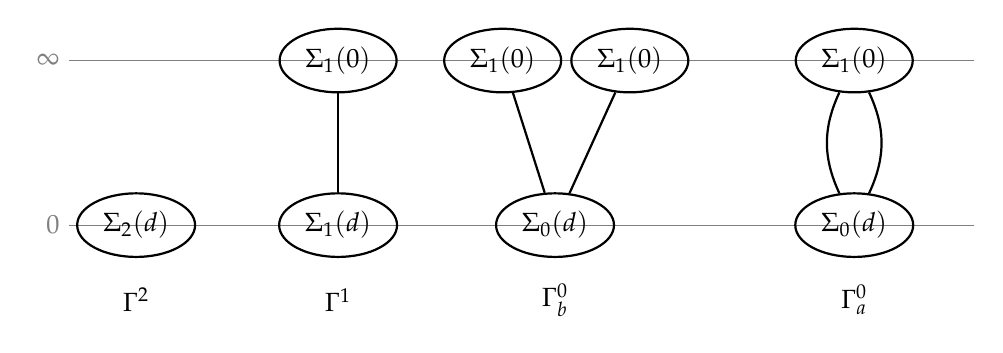
\begin{tikzpicture}[scale=0.95,transform shape]
        \draw[gray] (-0.9,0) -- (11.2,0);
        \draw[gray] (-0.9,2.2) -- (11.2,2.2);
        \node[anchor=east,gray] at (-0.9,0) {$0$};
        \node[anchor=east,gray] at (-0.9,2.2) {$\infty$};
        \node[ellipse,draw,thick,minimum width=1.5cm,minimum height=0.75cm] (a) at (0,0) {$\Sigma_2(d)$};
        \node at (0,-1) {$\Gamma^2$};
        \node[ellipse,draw,thick,minimum width=1.5cm,minimum height=0.75cm] (b0) at (2.7,0) {$\Sigma_1(d)$};
        \node[ellipse,draw,thick,minimum width=1.5cm,minimum height=0.75cm] (b1) at (2.7,2.2) {$\Sigma_1(0)$};
        \draw[thick] (b0) -- (b1);
        \node at (2.7,-1) {$\Gamma^1$};
        \node[ellipse,draw,thick,minimum width=1.5cm,minimum height=0.75cm] (c0) at (5.6,0) {$\Sigma_0(d)$};
        \node[ellipse,draw,thick,minimum width=1.5cm,minimum height=0.75cm] (c1) at (4.9,2.2) {$\Sigma_1(0)$};
        \node[ellipse,draw,thick,minimum width=1.5cm,minimum height=0.75cm] (c2) at (6.6,2.2) {$\Sigma_1(0)$};
        \draw[thick] (c0) -- (c1);
        \draw[thick] (c0) -- (c2);
        \node at (5.6,-1) {$\Gamma_b^0$};
        \node[ellipse,draw,thick,minimum width=1.5cm,minimum height=0.75cm] (d0) at (9.6,0) {$\Sigma_0(d)$};
        \node[ellipse,draw,thick,minimum width=1.5cm,minimum height=0.75cm] (d1) at (9.6,2.2) {$\Sigma_1(0)$};
        \draw[thick] (d0) to[bend left=25] (d1);
        \draw[thick] (d0) to[bend right=25] (d1);
        \node at (9.6,-1) {$\Gamma_a^0$};
    \end{tikzpicture}
    \caption{亏格二的四个非恒定局部化图；每个顶点均画成相应的 Riemann 曲面分量。}%
    \label{fig:g2loc}
\end{figure}

这四个非恒定图在 ~\Cref{fig:g2loc} 中绘制，其贡献为
\begin{align*}
    \Cont_{\Gamma^2} &= \ab<>^{t,\mr{SQ}}_{2,0}, \\
    \Cont_{\Gamma^1} &= -\ab< \frac{-\frac{5}{2}H^3 + \frac{5}{24}H^4t^{-1}}{(t-5H)(t-5H-\psi)}>^{t,\mr{SQ}}_{1,1}, \\
    \Cont_{\Gamma_b^0} &= \ab< \frac{-\frac{5}{2}H^3+\frac{5}{24}H^4t^{-1}}{(t-5H)(t-5H-\psi_1)}, \frac{-\frac{5}{2}H^3+\frac{5}{24}H^4t^{-1}}{(t-5H)(t-5H-\psi_2)}>^{t,\mr{SQ}}_{0,2},
\end{align*}
对于双边图，记\(H_1 = H \otimes 1\)、\(H_2 = 1 \otimes H\)，则
\[ \Cont_{\Gamma_a^0} = \ab< \frac{\frac{5}{3}(H^3\otimes H^4 + H^4 \otimes H^3)t^{-1} + \frac{65}{24}H^4 \otimes H^4 t^{-2}}{(t-5H_1)(t-5H_1-\psi_1)(t-5H_2)(t-5H_2-\psi_2)}>^{t,\mr{SQ}}_{0,2}. \]
注意：这些关联子位于\(\P^4\)上，因此\(H^4\)存在且非零。

第五项来自度零图，即常数
\[ -2c_{2,0} = -\frac{5}{144}, \qquad c_{2,0} = -\frac{1}{2}N_{2,0} = \frac{5}{288}, \]
将五项相加，可得局部化的恒等式
\[ F_2^{\mr{SQ}}(q) = \Cont_{\Gamma^2} + \Cont_{\Gamma^1} + \frac{1}{2}\Cont_{\Gamma_a^0} + \frac{1}{2}\Cont_{\Gamma_b^0} - 2c_{2,0}, \]
其中两个\(\frac{1}{2}\)因子分别来自\(\Gamma_a^0\)与\(\Gamma_b^0\)的自同构。

设\(Q = qe^{\tau(q)}\)与\(L = (1-5^5q)^{-1/5}\)，其中\(\tau(q) = I_1(q)/I_0(q) - \log q\)为普通镜像平移。现在应用稳定商壁交叉，可得精确恒等式
\[ F_2^{\mr{GW}}(Q) = I_0(q)^2 F_2^{\mr{SQ}}(q). \]
引入\(D_u = L^{-1}q\odv{}{q}\)及生成元
\[ \mc{X}_k = D_u^k \log \frac{I_0}{L}, \qquad \mc{Y}_k = D_u^k \log \frac{I_0I_{1,1}}{L^2}, \qquad I_{1,1} = 1 + q \odv{\tau}{q}, \quad D_u L = \frac{1}{5}(L^5-1), \]
各扭曲图的贡献涉及额外生成元。对我们的关键点在于，上述线性组合中这些项相互抵消，仅保留精确的有限生成性变量。记\(X = \mc{X}_1\)与\(Y_1 = \mc{Y}_1\)，可得
\begin{align*}
    F^{\mr{GW}}_2(Q) = \frac{I_0^2}{L^2}\Big(&\frac{70}{9}\mc{X}_3 + \frac{575}{18}X\mc{X}_2 + \frac{557}{72}X^3 + \frac{5}{6}Y_1\mc{X}_2 \\
    &- \frac{629}{72}Y_1X^2 - \frac{23}{24}Y_1^2 X - \frac{1}{24}Y_1^3 \\
    &+ \frac{125}{36}\mc{X}_2 L^4 - \frac{5}{24}X^2L^4 - \frac{35}{9}Y_1XL^4 - \frac{5}{24}Y_1^2L^4 \\
    &- \frac{1441}{300}XL^3 - \frac{41}{300}Y_1L^3 + \frac{31459}{7200}XL^8 + \frac{2141}{7200}Y_1L^8 \\
    &+ \frac{29621}{12000}L^{12} - \frac{116369}{36000}L^7 + \frac{547}{750}L^2\Big).
\end{align*}
若在大半径处展开，则可得
\[ F_2^{\mr{GW}}(Q) = -\frac{5}{144} + \frac{575}{48}Q + \frac{5125}{2}Q^2 + \frac{7930375}{6}Q^3 + O(Q^4), \]
这些系数即为 Gromov--Witten 不变量\(N_{2,d}\)，而非 ~\Cref{tab:quinticbps} 的 BPS 整数。

现在转向形式路径。\(\Omega^{\lambda}_{2,0}\)的 Givental--Teleman 公式是七个亏格二无腿稳定图之和，见~\Cref{fig:g2stable}。这里只需要\(R^{-1}(z)\)到\(z^3\)项；平移作用把这七种拓扑展开成\(17\)个带装饰的分层。

\begin{figure}[htpb]
    \centering
    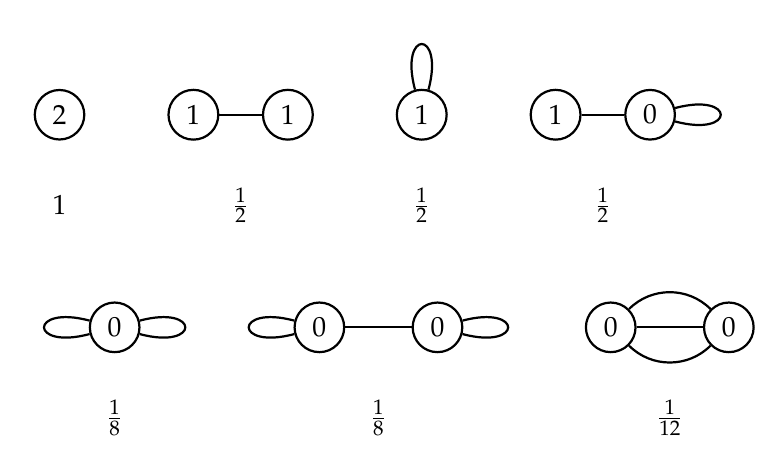
\begin{tikzpicture}[scale=1,transform shape,every loop/.style={min distance=8mm,looseness=10}]
        \node[circle,draw=black,thick] (a) at (0,0) {$2$};
        \node at (0,-1.15) {$1$};

        \node[circle,draw=black,thick] (b1) at (1.7,0) {$1$};
        \node[circle,draw=black,thick] (b2) at (2.9,0) {$1$};
        \draw[thick] (b1) -- (b2);
        \node at (2.3,-1.15) {$\frac{1}{2}$};

        \node[circle,draw=black,thick] (c) at (4.6,0) {$1$};
        \draw[thick] (c) edge[loop above] (c);
        \node at (4.6,-1.15) {$\frac{1}{2}$};

        \node[circle,draw=black,thick] (d1) at (6.3,0) {$1$};
        \node[circle,draw=black,thick] (d2) at (7.5,0) {$0$};
        \draw[thick] (d1) -- (d2);
        \draw[thick] (d2) edge[loop right] (d2);
        \node at (6.9,-1.15) {$\frac{1}{2}$};

        \node[circle,draw=black,thick] (e) at (0.7,-2.7) {$0$};
        \draw[thick] (e) edge[loop left] (e);
        \draw[thick] (e) edge[loop right] (e);
        \node at (0.7,-3.85) {$\frac{1}{8}$};

        \node[circle,draw=black,thick] (f1) at (3.3,-2.7) {$0$};
        \node[circle,draw=black,thick] (f2) at (4.8,-2.7) {$0$};
        \draw[thick] (f1) -- (f2);
        \draw[thick] (f1) edge[loop left] (f1);
        \draw[thick] (f2) edge[loop right] (f2);
        \node at (4.05,-3.85) {$\frac{1}{8}$};

        \node[circle,draw=black,thick] (g1) at (7.0,-2.7) {$0$};
        \node[circle,draw=black,thick] (g2) at (8.5,-2.7) {$0$};
        \draw[thick] (g1) -- (g2);
        \draw[thick] (g1) to[bend left=45] (g2);
        \draw[thick] (g1) to[bend right=45] (g2);
        \node at (7.75,-3.85) {$\frac{1}{12}$};
    \end{tikzpicture}
    \caption{亏格二、无腿的七个稳定图。顶点标有其亏格，每个图的权重为\(\frac{1}{\ab|\Aut\Gamma|}\)。幻灯片中，每个顶点均画成相应的 Riemann 曲面分量。}%
    \label{fig:g2stable}
\end{figure}

\begin{rmk}
    这些是稳定曲线的对偶图，而非~\Cref{fig:tropgraphs}的图，后者是通过将对数 GLSM的约化理论应用于热带分解公式所得到的刚性热带型。这里的两组拓扑结构恰巧重合，但每种情况下顶点的含义不同：在这里，它代表域曲线的一个分支，携带一个拓扑场论张量；在那里，它则是一个双分图热带曲线的层级，携带对数结构或\(\infty\)-顶点模问题。
\end{rmk}

对于形式化的路径，我们通过内在方式定义归一化的势
\[ P_2^{\lambda} \coloneqq \frac{Y}{I_0^2}F_2^{\lambda}, \qquad Y = L^5. \]
将完整的图求和约束于\(\Q[L,\mc{X}_1,\mc{X}_2,\mc{X}_3,\mc{Y}_1]\)，其等于
\begin{align*}
    P_2^{\lambda} ={}& -\frac{1}{128}L^{12} - \frac{23}{960}L^8\mc{X}_1 - \frac{9}{640}L^8\mc{Y}_1 + \frac{109}{16000}L^7 \\
    &- \frac{3}{80}L^4\mc{X}_1^2 - \frac{19}{320}L^4\mc{X}_1\mc{Y}_1 - \frac{3}{80}L^4\mc{Y}_1^2 - \frac{1}{64}L^4\mc{X}_2 \\
    &+ \frac{19}{1920}L^3\mc{X}_1 - \frac{47}{48000}L^2 \\
    &- \frac{67}{1152}\mc{X}_1^3 - \frac{101}{1152}\mc{X}_1^2\mc{Y}_1 - \frac{5}{48}\mc{X}_1\mc{Y}_1^2 - \frac{1}{24}\mc{Y}_1^3 \\
    &- \frac{25}{288}\mc{X}_1\mc{X}_2 - \frac{1}{48}\mc{X}_2\mc{Y}_1 - \frac{19}{1152}\mc{X}_3.
\end{align*}
为清晰起见，此即精确的\(\lambda\)扭曲答案，而非\(F_2^{\mr{GW}}\)。另请注意，\(Y = L^5\)为判别生成元，而\(\mc{Y}_1\)为对数导数生成元。

\subsection{有限生成性与扩展族}%
\label{sub:Finite generation and the extended family}

回顾前述有限生成环\(\mc{R} = \Q[A,B_1,B_2,B_3,Y]\)，赋予它分次
\[ \deg A = \deg B_1 = 1, \qquad \deg B_2 = 2, \qquad \deg B_3 = 3, \qquad \deg Y = 0. \]
对前述\(\phi_k = I_{1,1}\cdots I_{k,k}H^k\)，设
\[ \wt{\Omega}^{\lambda}_{g,n} \coloneqq 5^{g-1}\ab(\frac{Y}{I_0^2})^{g-1}\Omega^{\lambda,\tau}_{g,n}. \]

\begin{thm}[分次有限生成性 {\cite{GJRstructure}}]%
\label{thm:graded finite generation}
我们有
    \[ \wt{\Omega}^{\lambda}_{g,n}(\phi_{a_1}, \ldots, \phi_{a_n}) \in \bigoplus_{k \geq 0}\lambda^{5k}H^{2(3g-3+\sum_i a_i - 5k)}(\Mbar_{g,n},\Q)\otimes \mc{R}_{3g-3+\sum_i a_i}. \]
因此，组装二分剩余图后，扩展族的非等变分量满足
    \[ P^{\mbf{C}}_{g,n} = 5^{1-g}\int_{\Mbar_{g,n}}\wt{\Omega}^{\mbf{C}}_{g,n}(\phi_1^{\otimes n}) = \ab( \frac{Y}{I_0^2})^{g-1}\int_{\Mbar_{g,n}}\Omega^{\mbf{C}}_{g,n}(\phi_1^{\otimes n}) \in \mc{R}_{3g-3+n}. \]
\end{thm}

特别地，对固定的\((g,n)\)，只会出现有限多个分次单项式；\(R\)-矩阵也只有不超过\(3g-3+n\)阶的项可能贡献。

我们通过二分图求和组织扩展理论
\[ \Omega^{\mbf{C},\lambda}_{g,n} = \sum_{\Gamma \text{ 二部}} \frac{1}{\ab|\Aut\Gamma|}\prod_{v\in V_{\infty}(\Gamma)} C^{\infty}_{g_v,\mu_v}(\mbf{C};\vec{a}_v) \prod_{v \in V_0(\Gamma)}C^{\lambda}_{g_v,\vec{\delta}_v}(\vec{a}_v)\prod_{e \in E(\Gamma)}V_e, \]
其中\(C^{\infty}\)是有效或亚纯顶点因子，\(C^{\lambda}\)是形式零顶点关联子，\(\mu_v\)与\(\vec{\delta}_v\)记录相邻边的次数，\(V_e\)是边因子。只有完成整个图求和之后才取\(\lambda \to 0\)极限。令\(\mbf{C}=0\)，只留下形式\(\lambda\)-扭曲理论的主导扇区；令\(\mbf{C}=\mbf{C}^{\mr{eff}}\)并取\(\lambda\to0\)，则恢复五次三维簇的 Gromov--Witten 理论。对通用边求导会把该边切开，从而产生全纯反常方程，而有效顶点保持不变。

为推导全纯反常方程，写出\(P^{\mbf{C}}_g \coloneqq P^{\mbf{C}}_{g,0}\)并引入
\[ \mc{U} = B_1, \qquad \mc{V} = A + 2B_1, \qquad \mc{V}_2 = D\mc{U} + \mc{U}^2 - \mc{U}\mc{V}, \qquad \mc{V}_3 = (D+\mc{V})\mc{V}_2, \]
两个非全纯方向
\[ \partial_1 = \partial_{\mc{U}}, \qquad \partial_0 = \partial_{\mc{V}} - \mc{U}\partial_{\mc{V}_2} - \mc{U}^2\partial_{\mc{V}_3}. \]

\begin{thm}[扩展族的全纯反常方程 {\cite{GJRstructure}}]
我们有
    \[ -\partial_0 P^{\mbf{C}}_g = \frac{1}{2}P^{\mbf{C}}_{g-1,2} + \frac{1}{2}\sum_{\substack{g_1+g_2=g\\g_1,g_2\geq1}}P^{\mbf{C}}_{g_1,1}P^{\mbf{C}}_{g_2,1}, \qquad -\partial_1 P^{\mbf{C}}_g = 0. \]
\end{thm}

我们通过 ~\Cref{sub:The holomorphic anomaly equation} 的切割论证来证明这一点，因为\(R\)-矩阵传播子的导数很简单
\[ 5\mc{B}_{\partial_0} = \bar{\phi}_1 \otimes \bar{\phi}_1, \qquad 5\mc{B}_{\partial_1} = \bar{\phi}_0\otimes\bar{\phi}_2 + \bar{\phi}_2\otimes\bar{\phi}_0. \]
\(R^{-1}\)与每条边的导数仍落在同一个分次环中。因此，切开一条求过导的边后，结果闭合于\(\mc{R}\)中的低亏格关联子。令\(\mbf{C}=0\)，便得到形式\(\lambda\)-扭曲理论的同一组方程。

\subsection{边界条件}%
\label{sub:Boundary conditions}

我们用两类边界条件来约束全纯模糊性。

首先，我们在 orbifold 或 Landau-Ginzburg 点\(q = \infty\)处使用正则性，等价于\(L \to 0\)。对于形式或组装后的扩展势\(F_g^{\star}\)，设定
\[ \mc{P}_g^{\mr{orb},\star} \coloneqq \ab(\frac{L}{I_0})^{2g-2}F_g^{\star} = \Phi_g^{\star}(\mc{X}_1,\mc{X}_2,\mc{X}_3,\mc{Y}_1,L^{-1},L^5). \]
\Cref{thm:graded finite generation}限制了\(L\)可能出现的 Laurent 幂。形式 LG/CY 对应表明：经过解析延拓，并识别归一化的 CY 基与 LG 基之后，同一个形式\(R\)-矩阵多项式描述两个相。因此
\[ \lim_{L\to0}\Phi_g^{\star}(\mc{X}_1,\mc{X}_2,\mc{X}_3,\mc{Y}_1,L^{-1},L^5) \text{ 存在}, \]
若\(f_g(Y) = \sum_{i=0}^{3g-3}a_{i,g}Y^i\)且\(Y=L^5\)，五次三维簇的界为
\[ a_{i,g} = 0 \qquad \text{当 } i \leq \ceil*{\frac{3(g-1)}{5}}. \]
注意，这一陈述针对组装并归一化后的图贡献，而不是单个未经组装的亚纯顶点或橡胶顶点关联子。

其次，考察 conifold 点。令
\[ q = 5^{-5}(1+t_c)^{-1}, \qquad T_c = \frac{I_1^{\mr{co}}(t_c)}{I_0^{\mr{co}}(t_c)}, \]
其中\(I_0^{\mr{co}}, I_1^{\mr{co}}\)是一对局部 conifold 周期，并归一化为消失平坦坐标\(T_c\)在 conifold 点满足\(T_c=0\)。给定有限生成数据中的有理表达式\(f\)，把所有生成元关于\(T_c\)的 Laurent 展开代入，便得到其 conifold 值\(f^{\mr{co}}\)。\Cref{thm:graded finite generation}给出极点阶数界
\[ F_g^{\mbf{C},\mr{co}} = O\ab(T_c^{-(2g-2)}), \]
但我们需要更强的 \textit{间隙} 条件
\[ F_g^{\mr{co}} = \frac{c_g}{T_c^{2g-2}} + O(1), \]
即所有中间负幂\(T_c^{-(2g-3)}, \ldots, T_c^{-1}\)均消失。这是\(2g-2\)个条件，且不被有限生成性所蕴含。

\begin{conj}[形式 conifold 间隙]%
\label{conj:formal conifold gap}
形式\(\lambda\)-扭曲势具有通用主导项
    \[ F_g^{\lambda,\mr{co}} = \frac{(-1)^{g-1}B_{2g}}{2g(2g-2)T_c^{2g-2}} + O(1), \]
其中\(B_{2g}\)是伯努利数。
\end{conj}

\begin{exm}
在亏格二时，计算得到的展开为
    \[ F_2^{\lambda,\mr{co}} = \frac{1}{240T_c^2} + \frac{31}{6000} - \frac{7169}{3600000}T_c + \frac{22951}{45000000}T_c^2 + O(T_c^3). \]
    这给出的是亏格二的间隙，而不只是极点阶数的上界。
\end{exm}

我们还需考虑在其余图中出现的具有有理后裔插入的正式关联子，即
\[ C^{\lambda}_{g,\vec{\delta}}(\vec{a}) \coloneqq \ab< \frac{H^{3-a_1}}{-5H\ab(-\frac{5H}{\delta_1}-\psi_1)}, \ldots, \frac{H^{3-a_n}}{-5H\ab(-\frac{5H}{\delta_n}-\psi_n)}>^{\lambda}_{g,n} \]
其中\(\delta_i \geq 1\)和\(a_i \in \ab\{0,1,2,3,4\}\)。

\begin{conj}[带特殊插入的正则性]%
\label{conj:special correlator regularity}
我们有\(\ab(C^{\lambda}_{g,\vec{\delta}}(\vec{a}))^{\mr{co}} = O(1)\)。
\end{conj}

固定\(\vec{a}\)和\(\vec{\delta}\)后，\(\psi\)-展开中的单项可能有极点。这里的断言针对完整的有理后裔插入；在进一步对\(\vec{a}\)作剩余图求和之前，其负幂已经相互抵消。它只涉及这些特定的形式关联子，并不声称每个未经组装的亚纯关联子都正则。

我们可以利用~\Cref{conj:formal conifold gap,conj:special correlator regularity}将间隙转移到五次Gromov--Witten 理论中。剩余图的贡献形式为
\[ \sum_{\vec{a}} \prod_{v \in V_{\infty}(\Gamma)}I_0^{2g_v-2+\ell(\mu_v)}C^{\infty}_{g_v,\mu_v}(\vec{a}_v)\prod_{v\in V_0(\Gamma)}C^{\lambda}_{g_v,\vec{\delta}_v}(\vec{a}_v), \]
而\(C^{\infty}\)因子是\(q\)的有限多项式，所以在 conifold 点正则。形式理论的主导间隙与特殊关联子的正则性合在一起，便推出扩展族的间隙，继而推出五次三维簇的间隙。

\begin{rmk}
    \Cref{conj:formal conifold gap,conj:special correlator regularity}在一般情形仍是未解决的猜想，但郭帅、Janda 与阮勇斌已在五次三维簇上验证到\(g \leq 5\)。扩展族的极点阶数界是定理；间隙则依赖上述两个猜想，不过在\(g \leq 5\)时也已由显式计算证明。因此，在这些讲座举行时，五次三维簇 Gromov--Witten 理论的全亏格间隙是条件性结论，而\(g \leq 5\)时无条件成立。\footnote{此后，Chang--Guo--You--Zhang 在~\cite{CGYZ2026} 中宣布了五次三维簇 Gromov--Witten 理论的全亏格 conifold 间隙的证明。上面的两个形式理论猜想是另外的命题。}
\end{rmk}

综上，先由 Picard--Fuchs 数据计算 Givental \(R\)-矩阵与算子\(S_{\tau}(z)\)，再得到形式稳定图和亚纯剩余图，利用全纯反常方程与有限生成性，最后施加 orbifold 与 conifold 边界条件，便可确定\(F_g^{\mr{GW}}\)。

\section{\texorpdfstring{局部\(\P^1\)高亏格 GW 理论的结构}{局部 P1 高亏格 GW 理论的结构}（郭帅）}%
\label{sec:Structure of higher-genus GW theory of local P1 (郭帅)}

本讲义基于与许景毅、张庆生的合作成果。

\subsection{\(X_p\)的几何}%
\label{sub:The geometry of Xp}

我们将考虑全空间
\[ X_p \coloneqq \on{Tot}\ab(\mc{O}_{\P^1}(p-1) \oplus \mc{O}_{\P^1}(-p-1)), \]
这是一个非紧 toric Calabi--Yau 三维簇。当\(p=0\)时，它就是 resolved conifold。

设\(N \simeq \Z^3\)为秩\(3\)的格，\(M \coloneqq \Hom(N,\Z)\)为其对偶格；把\(M\)等同于\(\T \simeq (\C^{\times})^3\)的特征标格。\(X_p\)的扇的一维锥由
\[ b_1 = (1-p,-1,1), \qquad b_2 = (0,1,1), \qquad b_3 = (1,0,1), \qquad b_4 = (0,0,1), \]
生成，而\(X_p\)以\(\T\)为开稠密子集。利用对偶向量\(e_3^{\vee} \in M\)，得到\textit{Calabi--Yau 子环面}
\[ \T' \coloneqq \ker\ab(\chi^{e_3^{\vee}} \colon \T \to \C^{\times}) \simeq (\C^{\times})^2, \]
其作用保持 Calabi--Yau 形式。toric 图由两个三角形组成，对应于环面作用的两个不动点。在第一个不动点处，\(\T'\)-作用的权重为
\[ (0,1), \qquad (1,0), \qquad (-1,-1), \]
而在第二个不动点处，它们为
\[ (0,-1), \qquad (1,1-p), \qquad (-1,p). \]
因此，可以在这两个不动点处作局部化，把不变量表示为等变上同调中的量。这里\(H^*_{\T'}(\mr{pt}) = \C[\lambda_1,\lambda_2]\)。

当\(p \geq 2\)时，\(X_p\)的 toric 图不是凸的，因而\(X_p\)并非半射影。这正是现有文献没有涵盖这一情形的原因；我们将在~\Cref{sub:Topological recursion and the remodeling conjecture}中进一步解释。

\subsection{CGMPS 猜想}%
\label{sub:The conjecture of CGMPS}

2007 年，Caporaso、Griguolo、Mari\~{n}o、Pasquetti 与 Seminara 研究了\(X_p\)的 Gromov--Witten 理论。记
\[ \check{F}^{X_p}(w,\hbar) \coloneqq \sum_{g \geq 0} \check{F}_g^{X_p}(w) \hbar^{2g-2} \]
为总自由能。他们精确计算了亏格一部分，并提出如下 Ansatz：
\begin{equation}\label{eqn:cgmps ansatz}
    \check{F}_g^{X_p} = \frac{\wt{\mc{P}}_g(w,p)}{(w-w_c)^{5g-5}}, \qquad \wt{\mc{P}}_g(w,p) = \sum_{i=1}^{5g-5} a_{g,i}(p)(w-1)^i
\end{equation}
对于\(g \geq 2\)。此处，变量\(w\)与 Kähler 参数\(q\)通过\(w = 1-q\)和\(w_c = 1 - \frac{1}{p^2}\)相关联。我们的约定在\(F_g^{X_p} = (-1)^{g-1}\check{F}_g^{X_p}\)方面与\(g \geq 2\)不同。

分析亏格-零不变量的渐近行为，CGMPS 定义了缩放弦耦合常数为
\[ z^{5/2} = \hbar^{-2} \frac{p^8}{4w_c^5}(w-w_c)^5 \]
并引入了 \textit{双标度极限} \(F_{\mr{ds}}(z)\)，该量由\(\check{F}^{X_p}(w,\hbar)\)在令\(w \to w_c\)和\(\hbar \to 0\)且\(z\)固定时得到。将他们的亏格-零和亏格-一阶结果与 Ansatz 结合可得
\[ F_{\mr{ds}}(z) = -\frac{4}{15}z^{5/2} - \frac{1}{48}\log z + \sum_{g \geq 2} b_g z^{-5(g-1)/2}, \]
其中\(b_g = \ab(\frac{p^8}{4w_c^5})^{g-1}\wt{\mc{P}}_g(w_c,p)\)。

\begin{conj}[CGMPS {\cite{CGMPS2007}}]%
\label{conj:cgmps}
    双标度极限\(F_{\mr{ds}}(z)\)与\(F_{(3,2)}(z)\)（即\((3,2)\)的极小模型的自由能）一致。
\end{conj}

\((3,2)\)极小模型的自由能形式为
\[ F_{(3,2)}(z) = -\frac{4}{15}z^{5/2} - \frac{1}{48}\log z + \sum_{g\geq2} a_g z^{-5(g-1)/2}, \quad a_g = \frac{4^{1-g}}{(3g-3)!}\ab<\tau_2^{3g-3}>_g, \]
其中
\[ \ab<\tau_2^{3g-3}>_g \coloneqq \int_{\Mbar_{g,3g-3}} \psi_1^2 \cdots \psi_{3g-3}^2, \]
因此，我们看到 ~\Cref{conj:cgmps} 等价于对所有\(g \geq 2\)成立的陈述：\(b_g = a_g\)。

\subsection{主要结果}%
\label{sub:The main results (Guo local P1)}

~\Cref{sec:Structure of higher-genus GW invariants of the quintic (郭帅)}中的全局镜像对称框架在这里同样适用。目标是描述\(F_g^{X_p}\)在一维 B 模型模空间三个边界点附近的行为。极限\(q \to 0\)是大复结构极限，给出 A 模型变量\(Q\)下的 Gromov--Witten 展开；在\(q \to 1\)处，我们用带 framing 的\(R\)-矩阵证明\(F_g\)正则。更有意思的是，\(q \to \frac{1}{p^2}\)是一个高阶临界点。不同于普通 conifold 点的亏格\(g\)主导极点阶数\(2g-2\)，这里的退化允许最高\(5g-5\)阶极点；其主导系数由\((3,2)\)极小模型决定。

\begin{thm}%
\label{thm:local P1 mirror symmetry}
对于任意整数\(p \geq 2\)和\(g \geq 2\)，\(X_p\)的 Gromov--Witten 势由谱曲线\(\mc{C}\)的 Eynard-Orantin 拓扑递归计算得出，即
    \[ F_g^{X_p}(Q) = (-1)^{g-1}\mc{F}_g^{X_p}(q). \]
\end{thm}

特别地，这给出重构猜想的一个非半射影 toric Calabi--Yau 例子。

\begin{thm}%
\label{thm:local P1 rationality}
    对于\(g \geq 2\)，势\(F_g^{X_p}\)是一个有理函数的展开式
    \[ F_g^{X_p} = (-1)^{g-1}\frac{\mc{P}_g(\Delta,p^2)}{\Delta^{5g-5}}, \qquad \Delta \coloneqq \frac{1-p^2q}{1-q} = \frac{p^2(w-w_c)}{w}, \]
    其中\(\mc{P}_g \in \frac{1}{(p^2-1)^{2g-2}}\Q[p^2][\Delta]_{\leq 5g-5}\)。
\end{thm}

特别地，这证明了结构 Ansatz ~\Cref{eqn:cgmps ansatz}。

为识别双标度极限，仍需确定\(\mc{P}_g\)在\(\Delta = 0\)处的常数项。

\begin{thm}%
\label{thm:local P1 constant term}
    \(\mc{P}_g\)的常数项为
    \[ \mc{P}_g(0,p^2) = \frac{p^{6g-6}}{(p^2-1)^{2g-2}}\frac{1}{(3g-3)!}\ab<\tau_2^{3g-3}>_g. \]
\end{thm}

由于\(\wt{\mc{P}}_g(w_c,p) = \mc{P}_g(0,p^2)\ab(\frac{1}{p^2}-\frac{1}{p^4})^{5g-5}\)，\Cref{thm:local P1 constant term} 给出
\[ b_g = \frac{4^{1-g}}{(3g-3)!}\ab<\tau_2^{3g-3}>_g = a_g, \]
这证明了 ~\Cref{conj:cgmps}。

\subsection{\(X_p\)的 Gromov--Witten 理论}%
\label{sub:Gromov-Witten theory of Xp}

局部曲线的等变理论与局部化公式见~\cite{BryanPandharipande2008}。

由于\(X_p\)非紧，模空间\(\Mbar_{g,0}(X_p,d)\)并不固有，虚基本类的次数也无法直接定义。为定义这些不变量，我们引入环面作用，并转到\(\P^1\)上的扭曲理论，在那里应用虚拟局部化。

我们选择一个框架\(f \in \Z\)，并令\(\T_f \coloneqq \ker(\lambda_2 - f\lambda_1)\)。两个局部化权重行，每行包含一个零权重，为
\[ \begin{bmatrix} 0 & f & 1 & -f-1 \end{bmatrix}, \qquad \begin{bmatrix} -f & 0 & 1-fp+f & -1+fp \end{bmatrix}. \]
若\(f \neq 0\)，则缩放特征量可得到等价的对称权重向量
\[ \begin{bmatrix} 1 & -1 & -\mf{f} & \mf{f} \end{bmatrix}, \qquad \mf{f} = 1-p+\frac{2}{f}, \]
并记调整后的环面为\(\T_{\mf{f}}\)。若\(H^*_{\T_{\mf{f}}}(\mr{pt}) = \C[\lambda]\)，此归一化则
\[ \lambda_1 = -\frac{2}{\mf{f}}\lambda, \qquad \lambda_2 = -2\lambda. \]

令\(\pi \colon \Mbar_{g,1}(\P^1,d) \to \Mbar_{g,0}(\P^1,d)\)为遗忘映射，且令\(\ev\)为标记处的求值。则我们定义
\[ N^{X_p}_{g,d} \coloneqq \int_{[\Mbar_{g,0}(\P^1,d)]^{\vir}_{\T_{\mf{f}}}} e_{\T_{\mf{f}}}^{-1}\ab(R^{\bullet}\pi_* \ev^*(\mc{O}(p-1)\oplus\mc{O}(-p-1))), \]
其中\(e_{\T_{\mf{f}}}\)是等变欧拉类。对于\(p=0\)，此式特化为通常的解析锥公式。

我们得到一个 CohFT \(\Omega^{\lambda,\mf{f}}\)，其态空间为等变上同调环
\[ H^*_{\T_{\mf{f}}}(\P^1) = \frac{\C[H,\lambda]}{(H+\lambda)(H-\lambda)} \]
和配对
\[ (a,b) \coloneqq \int_{\P^1} a \cup b \cup e^{-1}_{\T_{\mf{f}}}(\mc{O}(p-1)\oplus\mc{O}(-p-1)). \]
在平坦基\(\ab\{\1,H\}\)中，Gram 矩阵由
\[ \frac{1}{((p-\mf{f})^2-1)((p+\mf{f})^2-1)}\begin{pmatrix} 2\mf{f}p\lambda^{-3} & (1-\mf{f}^2-p^2)\lambda^{-2} \\ (1-\mf{f}^2-p^2)\lambda^{-2} & 2\mf{f}p\lambda^{-1} \end{pmatrix}. \]
我们定义关联子为
\[ \Omega^{\lambda,\mf{f}}_{g,n}(\alpha_1,\ldots,\alpha_n) \coloneqq \sum_{d\geq0}\st_*\ab(\prod_{i=1}^n \ev_i^*\alpha_i \cap [\Mbar_{g,n}(\P^1,d)]^{\vir,\lambda,\mf{f}})e^{-dt}, \]
其中\(\st\)是遗忘映射到\(\Mbar_{g,n}\)。扭曲的虚拟类由
\[ [\Mbar_{g,n}(\P^1,d)]^{\vir,\lambda,\mf{f}} \coloneqq e^{-1}_{\T_{\mf{f}}}\ab(R^{\bullet}\pi_*\ev^*(\mc{O}(p-1)\oplus\mc{O}(-p-1))) \cap [\Mbar_{g,n}(\P^1,d)]^{\vir}_{\T_{\mf{f}}}. \]
设\(Q = (-1)^{p+1}e^{-t}\)。则亏格-\(g\)势由
\[ F^{X_p}_g(t) = \int_{\Mbar_g} \Omega^{\lambda,\mf{f}}_{g,0}. \]

\begin{rmk}
    度为正的不变量\(N^{X_p}_{g,d\geq1}\)通过拓扑顶点~\cite{LLLZ2009} 与\(\mf{f}\)无关，且其\(\lambda\)独立性也源自 ~\Cref{thm:local P1 reconstruction}。在证明 ~\Cref{thm:local P1 rationality} 时，我们将利用\(\mf{f}\)的独立性。
\end{rmk}

在亏格零中，我们有
\[ N^{X_p}_{0,d} = \frac{(-1)^{(p+1)d-1}}{d^3}\binom{p^2d-1}{d-1}, \qquad d \geq 1, \]
这使得我们能够精确计算 Yukawa 耦合：
\[ Y = -\partial_t^3 F_0^{X_p}(t) = \frac{1-\mf{f}^2-p^2}{((p-\mf{f})^2-1)((p+\mf{f})^2-1)} + \frac{q}{p^2q-1}. \]
此处，\(q\)与\(Q\)通过镜像映射\(Q = q(1-q)^{p^2-1}\)相关联。利用\((v_1 \star v_2, v_3) = \Omega^{\lambda,\mf{f}}_{0,3}(v_1,v_2,v_3)\)评估量子乘积，我们得到
\[ H \star H = -\frac{(\mf{f}^2-1)q+1}{p^2q-1}\lambda^2 \1 - \frac{2\mf{f}pq}{p^2q-1}\lambda H, \]
或以矩阵形式表示为
\[ H \star = \begin{pmatrix} 0 & -\frac{(\mf{f}^2-1)q+1}{p^2q-1}\lambda^2 \\ 1 & -\frac{2\mf{f}pq}{p^2q-1}\lambda \end{pmatrix}. \]
该矩阵的特征值\(L_{\alpha}\)通常互异。因此\(\Omega^{\lambda,\mf{f}}\)是半单的。我们用\(\ab\{e_{\alpha}\}\)表示幂等基，\(\Delta_{\alpha}^{-1} = (e_{\alpha},e_{\alpha})\)表示长度，以及\(\bar{e}_{\alpha} \coloneqq \Delta_{\alpha}^{1/2}e_{\alpha}\)表示归一化的标准基。

由于该理论是半单的，\Cref{thm:teleman} 给出
\[ \Omega^{\lambda,\mf{f}} = R.T_R.\ab(\bigoplus_{\beta=0}^1 \Omega^{\mr{KW}}_{\beta}), \]
其中\(\Omega^{\mr{KW}}_{\beta}\)是一维的平凡 CohFT，且\(T_R(z) = z(\wt{\1}-R^{-1}(z)\1)\)满足\(\wt{\1} \coloneqq \sum_{\beta}\bar{e}_{\beta}\)。我们从量子微分方程确定\(R\)矩阵
\[ z \d{S_{\tau}(z)} = \d{\tau} \star_{\tau} S_{\tau}(z). \]
等变局部化与量子 Riemann-Roch 将基本解与\(R\)矩阵通过
\[ (S^*_{\tau}(z)\1, \bar{e}_{\alpha})\big|_{q=0}\, C_{\alpha}(z) = (\1, R(z)\bar{e}_{\alpha})e^{u^{\alpha}(q)/z}, \]
其中初始条件\(C_{\alpha}(z)\)是涉及伯努利数的指数函数。将\(R_{i\bar{\alpha}}(z) \coloneqq (R^*(z)H^i, \bar{e}_{\alpha})\)代入量子微分方程，我们得到二阶方程
\[ \ab( (zD+L_{\alpha})^2 + \frac{2\mf{f}pq}{p^2q-1}\lambda(zD+L_{\alpha}) + \frac{(\mf{f}^2-1)q+1}{p^2q-1}\lambda^2 )R_{0\bar{\alpha}} = 0, \]
其中\(D = -\partial_t\)。我们可按\(z\)的阶次逐阶计算\(R\)矩阵。

\subsection{拓扑递归与重构猜想}%
\label{sub:Topological recursion and the remodeling conjecture}

我们现转向B模型侧。我们的目标是将拓扑递归与上述Givental-Teleman重构相匹配。Eynard--Orantin 的拓扑递归~\cite{EO2007} 接受输入为 \textit{谱曲线} 与\((\Sigma,x,y,B)\)，其中\(\Sigma\)是一个 Riemann 曲面；\(x\)以局部有理函数微分\(\d{x}\)定义，该微分在有限个单零点处有零；\(y\)在这些零点附近全纯，且\(\d{y} \neq 0\)处不为零；\(B\)是定义在\(\Sigma \times \Sigma\)上的基本双微分。在\(\d{x}\)的零点\(z^{\beta}\)附近，令\(\bar{z} \neq z\)为局部共轭点，满足\(x(\bar{z}) = x(z)\)，并定义递归核
\[ K_{\beta}(z_0,z) \coloneqq \frac{\int_{\bar{z}}^z B(z_0,z')}{2(y(z)-y(\bar{z}))\d{x}(z)}. \]
若我们设定\(\omega_{0,0} = \omega_{1,0} = 0\)、\(\omega_{0,1}(z) = y(z)\d{x}(z)\)以及\(\omega_{0,2}(z_1,z_2) = B(z_1,z_2)\)，则对\(2g-2+n+1 > 0\)的多微分递归定义为
\begin{align*}
    \omega_{g,n+1}(z_0,z_{[n]}) ={}& \sum_{\beta}\on{Res}_{z = z^{\beta}} K_{\beta}(z_0,z) \\
    &\cdot \Bigg( \omega_{g-1,n+2}(z,\bar{z},z_{[n]}) \\
    &\qquad + \sideset{}{'}\sum_{\substack{g_1+g_2 = g \\ I \sqcup J = [n]}}\omega_{g_1,\abs{I}+1}(z,z_I)\omega_{g_2,\abs{J}+1}(\bar{z},z_J)\Bigg),
\end{align*}
其中带撇的和排除\(\omega_{0,1}\)。对于\(g \geq 2\)，自由能由
\[ \mc{F}_g = \omega_{g,0} \coloneqq \frac{1}{2-2g}\sum_{\beta}\on{Res}_{z=z^{\beta}}\omega_{g,1}(z)\int_{z'=z^{\beta}}^z \omega_{0,1}(z'). \]

Bouchard、Klemm、Mari\~{n}o 与 Pasquetti 的重构猜想~\cite{BKMP2009} 断言：环面Calabi--Yau 三维簇\(X\)的全亏格开、闭Gromov--Witten 不变量，等于其镜像曲线上由拓扑递归产生的不变量\(\omega_{g,n}\)。陈琳与 Zhou 分别证明了\(\C^3\)的开弦情形。\footnote{陈琳在 \href{https://arxiv.org/abs/0910.3739}{arXiv:0910.3739} 中利用了他在 \href{https://arxiv.org/abs/0709.1738}{arXiv:0709.1738} 中建立的 Mari\~{n}o--Vafa 公式的对称化 cut-and-join 方程。陈琳、李逸与刘克峰此前在 \href{https://arxiv.org/abs/math/0609263}{arXiv:math/0609263} 中用 Hurwitz 数的对称化 cut-and-join 方程推导了 Witten 猜想；前述2007年论文第5节对该猜想的推导沿用了这一思路。} Eynard--Orantin 给出了光滑半射影环面Calabi--Yau 三维簇情形的证明；随后 Fang--Liu--Zong~\cite{FLZ2020} 将其推广至半射影环面Calabi--Yau 三维 orbifold。遗憾的是，当\(p \geq 2\)时，\(X_p\)并非半射影，因而不在该证明的适用范围内。

为比较两方，我们使用 Dunin-Barkowski、Orantin、Shadrin 与 Spitz~\cite{DOSS2014} 提出的重构，该重构将稳定的拓扑递归关联子与半单 CohFT 的 Givental 重构相匹配。在每个临界点\(z^{\beta}\)附近，定义局部 Airy 坐标\(\eta^{\beta}(z)\)为
\[ x(z) = x(z^{\beta}) + \frac{1}{2}(\eta^{\beta}(z))^2 \]
以及全局定义的有理函数参考形式
\[ \d{\zeta^{\bar{\beta}}}(z) \coloneqq -\on{Res}_{z'=z^{\beta}}\frac{B(z',z)}{\eta^{\beta}(z')}. \]
所关联的 CohFT 的状态空间\(V\)由对应于临界点的基\(\ab\{\bar{e}_{\beta}\}\)张成，且配对为对角矩阵，其元素为\(\eta(\bar{e}_{\beta},\bar{e}_{\gamma}) = \delta_{\beta,\gamma}\)。曲线\(R\)-matrix \(\check{R}\)由渐近拉普拉斯变换定义为
\[ \frac{u}{\sqrt{2\pi u}}\int_{\mc{L}_{\gamma}} e^{-x(z)/u}\d{\zeta^{\bar{\beta}}}(z) \asymp e^{-x^{\gamma}/u}\eta\ab(\bar{e}_{\gamma}, \check{R}^*(-u)\bar{e}_{\beta}), \]
而\(\d{y}\)的类似变换定义了\(T(u)\)；若所得 CohFT 具有平坦单位，则\(T(u) = u(\wt{\1}-\check{R}^{-1}(u)\1)\)。此时，\(\check{R}\)为辛结构，曲线 CohFT 为\(\check{\Omega} = \check{R}.T.\ab(\bigoplus_{\beta}\Omega^{\mr{KW}}_{\beta})\)，且若将\(\d{\zeta^{\bar{\beta}}_k} \coloneqq \ab(-\d{} \circ \frac{1}{\d{x}})^k \d{\zeta^{\bar{\beta}}}\)写为，对应关系为
\begin{align*}
    \omega_{g,n}(z_1,\ldots,z_n) ={}& \sum_{\substack{k_1,\ldots,k_n \geq 0 \\ \beta_1,\ldots,\beta_n \in [N]}}\ab(\int_{\Mbar_{g,n}} \check{\Omega}_{g,n}(\bar{e}_{\beta_1}\psi_1^{k_1},\ldots,\bar{e}_{\beta_n}\psi_n^{k_n})) \\*
    &\cdot \prod_{i=1}^n \d{\zeta^{\beta_i}_{k_i}}(z_i).
\end{align*}

对于\(X_p\)，我们将考虑谱曲线
\[ \mc{C}_{\mf{f}} = \ab(\P^1, x_{\mf{f}}(z), y(z), B(z_1,z_2) = \frac{\d{z_1}\d{z_2}}{(z_1-z_2)^2}), \qquad x_{\mf{f}}(z) = x(z) + 2\mf{f}\lambda^2 y(z), \]
其中
\begin{align*}
    x(z) &= t^0 + \lambda \log q + \lambda(p-1)\log z + \lambda(-p-1)\log\frac{q-z}{1-z}, \\
    y(z) &= \frac{p+1}{2\lambda}\log(1-q) + \frac{1}{2\lambda}\log z - \frac{1}{2\lambda}\log(1-z) - \frac{1}{2\lambda}\log(q-z).
\end{align*}
求解\(\d{x_{\mf{f}}} = 0\)，可得临界点
\[ z^{\alpha} = \frac{1-\ms{L}_{\alpha}}{1+\mf{f}+p\ms{L}_{\alpha}}, \qquad \ms{L}_{\alpha} = \lambda^{-1}L_{\alpha}, \qquad q = \frac{\ms{L}_{\alpha}^2-1}{(p\ms{L}_{\alpha}+1)^2-1}, \]
且内积由\(\eta(e_{\alpha},e_{\beta}) = \delta_{\alpha,\beta}\frac{y'(z^{\alpha})^2}{x''_{\mf{f}}(z^{\alpha})}\)给出。由此，所得长度满足\(\check{\Delta}_{\alpha} = \Delta_{\alpha}\)。因此，Frobenius 结构的谱曲线是量子乘积的\(X_p\)。

至此，我们已匹配了 Frobenius 结构，故尚需匹配两组\(R\)-matrices。在勒夫歇茨针状物上进行分部积分可得
\begin{align*}
    u \partial_{t^0}\ab(e^{-x^{\gamma}/u}\check{R}^*(-u)^{\bar{\gamma}}_{\1}) &= -e^{-x^{\gamma}/u}\check{R}^*(-u)^{\bar{\gamma}}_H, \\
    u\partial_{t^0}\ab(e^{-x^{\gamma}/u}\check{R}^*(-u)^{\bar{\gamma}}_H) &= -\lambda b(q)e^{-x^{\gamma}/u}\check{R}^*(-u)^{\bar{\gamma}}_H - \lambda^2 c(q) e^{-x^{\gamma}/u}\check{R}^*(-u)^{\bar{\gamma}}_{\1},
\end{align*}
其中
\[ c(q) = -\frac{(\mf{f}^2-1)q+1}{p^2q-1}, \qquad b(q) = -\frac{2\mf{f}pq}{p^2q-1} \]
正是上述计算得到的量子乘积的各项，因此这些结果与 Gromov-Witten 理论中对应的\(R\)矩阵的量子微分方程一致。为满足初始条件，我们取沿拇指的拉普拉斯变换在\(q \to 0\)处的极限，由此产生贝塔函数及其伽马函数的乘积。随后，斯特林展开式与伯努利数初始条件\(C_{\alpha}(z)\)相匹配。

\begin{prop}%
\label{prop:R matrices coincide}
两个\(R\)矩阵完全一致，即\(R(z) = \check{R}(u)|_{u=-z}\)。
\end{prop}

我们已证明，规范长度与\(R\)矩阵一致。在代换\(u = -z\)后，亏格-\(g\)与稳定图的和相差整体奇偶性\((-1)^{3g-3} = (-1)^{g-1}\)，从而证明 ~\Cref{thm:local P1 mirror symmetry}。

\subsection{有理性}%
\label{sub:Rationality}

由于高亏格势函数与\(\mf{f}\)无关，为简化起见令\(\mf{f} = 0\)。这样典范基和量子微分方程都会简化；后者变为
\[ \ab((zD+L_{\alpha})^2 - \frac{1-q}{1-p^2q}\lambda^2)R_{0\bar{\alpha}} = 0, \qquad L_{\alpha} = (-1)^{\alpha}\lambda L, \quad L = \ab(\frac{1-q}{1-p^2q})^{1/2}, \]
我们将\(R\)矩阵的项记为\((R_k)_i^{\alpha}\)。定义
\[ \Delta \coloneqq \frac{1}{L^2} = \frac{1-p^2q}{1-q}, \qquad \mc{R} \coloneqq \Q[p^2,\Delta], \qquad \mc{R}_{\leq d} \coloneqq \ab\{P \in \mc{R} \mid \deg_{\Delta} P \leq d\}. \]
现在，我们通过归纳法证明量子微分方程的系数具有多项式结构。

\begin{prop}%
\label{prop:R matrix polynomiality}
对于\(k \in \Z_{\geq0}\)且\(i = 0,1\)，有
    \[ (R_k)_i^{\alpha} \in \frac{1}{(p^2-1)^k \lambda^{k-i}\Delta^{(3k+i)/2}}\mc{R}_{\leq 2k}. \]
\end{prop}

分析 Givental-Teleman 重构中度贡献的稳定图和，并追踪\(\lambda\)、\(\Delta\)与\(p^2-1\)的幂次，可得以下结果。

\begin{thm}%
\label{thm:local P1 reconstruction}
将\([\,\cdot\,]_d\)定义为 codimension-\(d\)分量，有
    \begin{align*}
        \ab[\Omega^{\lambda}_{g,n}(H^{a_1},\ldots,H^{a_n})]_d \in{}& \frac{\lambda^{3g-3-d+\sum_i a_i}}{(p^2-1)^{d-(g-1)}\Delta^{\frac{1}{2}(g-1+3d+\sum_i a_i)}}\mc{R}_{\leq 2d} \\
        &\otimes H^{2d}(\Mbar_{g,n},\Q).
    \end{align*}
\end{thm}

取\(n=0\)与\(d = 3g-3 = \dim \Mbar_g\)代入 ~\Cref{thm:local P1 reconstruction}，可得
\[ F_g^{X_p} \in \frac{1}{(p^2-1)^{2g-2}\Delta^{5g-5}}\mc{R}_{\leq 6g-6}, \]
若~\Cref{thm:local P1 rationality}中度的分子在\(\Delta\)处受\(5g-5\)的限制，则可观察到该限制出现在\(q=1\)处。由于\(\Delta\)在此处存在简单极点，\(F_g^{X_p}\)的正则性要求分子必须抵消\(\Delta\)的最高幂次。因此，我们将有理性的问题归结为在\(q=1\)处的正则性。而这一正则性则源自\(\mf{f}\)下的\(F_g^{X_p}\)的独立性，以及当\(\mf{f} \neq 0\)时，\(R\)矩阵在\(q \to 1\)极限下的存在性。

\subsection{极限\(\Delta = 0\)}%
\label{sub:The limit Delta = 0}

为确定剩余的常数项，现研究极限\(\Delta = 0\)，其即为精确的双标度极限。我们通过重新缩放规范长度
\[ \delta_{\alpha} \coloneqq \Delta^{1/2}\Delta_{\alpha} = (-1)^{\alpha+1}2(p^2-1)\lambda^3 \]
并定义修改后的\(R\)矩阵项，即在 ~\Cref{prop:R matrix polynomiality} 中隔离\(\Delta = 0\)的主导项，具体为
\[ (\bar{R}_k)_i^{\alpha} \coloneqq \ab[(-1)^k (R_k)_i^{\alpha}\Delta^{(3k+i)/2}]\Big|_{\Delta=0}, \qquad i = 0,1. \]
则\(F_g^{X_p}\)的图求和在替换\(\Delta_{\alpha}\)为\(\delta_{\alpha}\)且\((R_k)_i^{\alpha}\)为\((\bar{R}_k)_i^{\alpha}\)后，可表示为\(\mc{P}_g(0,p^2)\)的公式。

\begin{lem}%
\label{lem:R matrix at Delta zero}
在\(\Delta = 0\)处求解一阶量子微分方程，可得闭式解
    \begin{align*}
        (\bar{R}_k)_0^{\alpha} &= \frac{p^{2k}}{(p^2-1)^k\lambda^k}(-1)^{k\alpha}\prod_{n=1}^k \frac{(6n-7)(6n+1)}{48n}, \\
        (\bar{R}_k)_1^{\alpha} &= \frac{p^{2k}}{(p^2-1)^k \lambda^{k-1}}(-1)^{(k-1)\alpha}\frac{1-6k}{1+6k}\prod_{n=1}^k \frac{(6n-7)(6n+1)}{48n}.
    \end{align*}
\end{lem}

在 ~\Cref{lem:R matrix at Delta zero} 中提取\(p\)依赖项后，我们得到纯有理系数。现在，我们构造在\(V = \on{span}\ab\{\phi_0,\phi_1\}\)上的拓扑场论\(\Omega^{\mr{top}}\)，其单位为\(\phi_0\)，其中
\[ (\phi_0,\phi_0) = (\phi_1,\phi_1) = 0, \qquad (\phi_0,\phi_1) = -1, \qquad \phi_1 \star \phi_1 = \phi_0. \]
通过应用\(R(z)\)及其平移单位重构，我们得到常数项\(C_g\)，其中
\[ \mc{P}_g(0,p^2) = \frac{p^{6g-6}}{(p^2-1)^{2g-2}}C_g, \]
还需确定重构的CohFT

\((2,3)\)极小模型具有谱曲线
\[ x(z) = \frac{1}{3}(z^3-3\ep^2 z) + \tau^0, \qquad y(z) = \frac{1}{2}(z^2-2), \]
其平坦坐标为\(\tau^1 = \ep^4/2\)。若令\(\tau^0 = 0\)、\(\ep = 1\)，并作识别\(\phi_0 = \partial_{\tau^0}\)和\(\phi_1 = \partial_{\tau^1}\)，则在\(\Delta = 0\)处由\(X_p\)得到的\(R\)-矩阵，与该曲线的\(R\)-矩阵一致。因此，\(C_g\)恰为\((2,3)\)极小模型的自由能。

最后，我们应用辛交换\((x,y) \mapsto (y,-x)\)，此时曲线变为
\[ x(z) = \frac{1}{2}(z^2-2), \qquad y(z) = -\frac{1}{3}(z^3-3z). \]
交换后的曲线具有一维态空间、平凡的\(R\)-matrix 以及平移\(T(u) = u^2 \bar{e}\)，使得
\[ C_g = \frac{1}{(3g-3)!}\ab<\tau_2^{3g-3}>_g, \]
即 ~\Cref{thm:local P1 constant term}。需注意，此交换对应于\((2,3)\)与\((3,2)\)最小模型之间的关系，因此此处出现的交数即为 ~\Cref{conj:cgmps}。

\printbibliography[title={参考文献}]

\end{document}

%%% Local Variables:
%%% mode: latex
%%% TeX-master: t
%%% End:
